%\documentclass[a4paper]{article}
\documentclass[11pt,a4paper,twoside]{report}
%style
%\usepackage[a4paper,top=3cm,bottom=2cm,left=3cm,right=3cm,marginparwidth=1.75cm]{geometry}
%%% text size %%%
\setlength{\topmargin}{10mm}
\addtolength{\topmargin}{-1in}
\setlength{\textheight}{262mm}
\setlength{\headsep}{5mm}
\setlength{\headheight}{0mm}
\setlength{\topskip}{0mm}
\setlength{\oddsidemargin}{-1in} %  set real left margin 0pt
\setlength{\evensidemargin}{-1in} % do
\addtolength{\oddsidemargin}{25mm} % odd page 25mm left margin
\addtolength{\evensidemargin}{15mm}% even page 15mm left margin
\setlength{\textwidth}{170mm}
%\setlength{\leftmargin}{-1 in}
\usepackage{float} %figure placement
%\pagestyle{fancy}
%\lhead[\it \scriptsize \leftmark]{}
%\chead[]{}
%\rhead[]{\it \scriptsize \rightmark}
%\renewcommand{\headrulewidth}{0.4pt}
%\renewcommand{\footrulewidth}{0pt}
%\renewcommand{\baselinestretch}{1.}
%\doublespacing

% Language and font encodings
\usepackage[english]{babel}
\usepackage[utf8x]{inputenc}
\usepackage[T1]{fontenc}
%\usepackage{subfig}
\usepackage{amsmath,amssymb,amsfonts}

%https://www.sharelatex.com/learn/Bibtex_bibliography_styles
%\bibliographystyle{apacite}
\bibliographystyle{alpha}
%\usepackage{natbib, aas_macros}
%\bibliographystyle{plainnat}
\usepackage{caption}
\usepackage{subcaption}
\usepackage{comment}
%for list/enumeration
\usepackage{enumitem} 
%for Japanese title
%\usepackage{CJKutf8} 
%for table
\usepackage{multirow} 
%\usepackage[colorinlistoftodos]{todonotes}
%for bibliography
%\usepackage{apacite}
%indent first paragraph
\usepackage{indentfirst}
\usepackage{graphicx}
\usepackage[colorlinks=true, allcolors=blue]{hyperref}


%\title{Ground-based Observations of Rayleigh Scattering in the Atmosphere of Low Density Exoplanets}
%(低密度太陽系外惑星の大気のレイリー散乱の地上観測)

\title{
  \Large{\bf Master's Course Thesis}\\[1.5cm]
  \LARGE{\bf Multi-color Simultaneous Transit Observations \\
of Low Density Hot Jupiters}\\[2cm]
%\begin{CJK}{UTF8}{min}\LARGE{\bf 低密度ホットジュピターに対する多色同時トランジット観測}\end{CJK} \\
}
\date{\Large{\bf January 29, 2018}}

\author{
  \Large{\bf Jerome Pitogo de Leon}\\
  \Large{\bf 35-166337}\\
 %\begin{CJK}{UTF8}{min}\LARGE{ジェローム \; ピトゴ \; デレオン}
 %\end{CJK}\\[1cm]
  \Large{\bf Department of Astronomy}\\
  \Large{\bf Graduate School of Science,
  The University of Tokyo}\\
 % \begin{CJK}{UTF8}{min}\LARGE{東京大学大学院理学系研究科}
 % \end{CJK}\\
}

\begin{document}

\maketitle
%\thispagestyle{empty}\mbox{}\newpage

\pagenumbering{roman}

\begin{abstract}
%intro
While the Kepler space mission was responsible for most of planet discoveries, the majority of the $\sim$523 planets with masses > 0.5 M$_J$ were discovered by ground-based surveys that are optimized to find giant planets in short-period orbits such as hot Jupiters. 
%motivation
Hot Jupiters remain prime targets for atmospheric studies from the ground thanks to their relatively large scale heights.
%observation
For this study, we used OAO/MuSCAT to conduct simultaneous multi-color observations of several transiting systems with known low-density Hot Jupiters including HAT-P-12b, HAT-P-14b, and WASP-21b. 
%Onitsuka  https://arxiv.org/pdf/1701.01588.pdf
%The data were obtained with the Multicolor Simultaneous Camera for studying Atmospheres of Transiting exoplanets (MuSCAT) on the 188 cm telescope at Okayama Astrophysical Observatory in Japan. We observed the fading event in the $g′_2$-, $r′_2$-, and $z_{s,2}$-bands simultaneously.
%goal
Our goals are (1) to improve the transit parameters of these systems and (2) to search for broad spectral features such as Rayleigh scattering signature in the optical wavelengths. 
%method, analysis
Our homogeneous analysis of transit light curves uses Bayesian modeling to determine the best estimates and Bayesian credible regions of the transit and systematics model parameters, taking into account the presence of correlated noise in the light curves.
%results
%%%-----------------------improved transit ephemerides
%The c 2 value of the linear fit is 15.5 for five degrees of freedom (DOF), meaning that the linear function nominally has a 2.6σ discrepancy with the observed data. However, discrepancies with similar levels often arise in ground-based T c observations, possibly due to unknown systematics rather than the true timing variations. Therefore, we do not consider it to be a noticeable TTV signal at this point. In any case, correction of the ephemeris in this work should be useful for future observations.
%%%-----------------------search for TDV
%Next we search for Transit Duration Variations (TDV) to check for any evidence of additional bodies. The measured b values of the seven transits and their uncertainties are listed in Table 5 and shown in Figure 5. A constant fit to these values gives the mean of b = 0.9015±0.0024 with c 2 = 7.5 for dof = 6, meaning that no significant variation is observed
%%%-----------------------atmospheric model

The derived transit parameters are in general agreement with previous results. 
%As a result, we find a significant wavelength dependence of fading depths of about 3.1\%, 1.7\%, 1.0\% for the $g′_2$-, $r′_2$-, and $z_{s,2}$-bands, respectively. A cloudless H/He dominant atmosphere of a hot Jupiter cannot explain this large wavelength dependence. Additionally, we rule out a scenario by the occultation of the gravity-darkened host star.
%%%-----------------------atmospheric model
Careful analysis of transit depth variation in each band show a marked increase in the planetary radius from the red toward the blue ends of the visible wavelength range.  
In addition, to compare the observed data with a theoretical atmospheric model, we calculate a model spectrum for the first time for each planet considering two cases: (case 1) 1 $\times$ Solar and (case 2) 100 $\times$ Solar metallicity clear atmospheres, assuming thermochemical equilibrium compositions and isothermal structures. 
Comparing the measured transit depths with the spectrum model for HAT-P-12b and HAT-P-44b help rule out stellar activity and site-specific systematics as the source of this variation. In addition, we obtained a broadband transmission spectrum in agreement with the atmospheric model of Sing et al. (2016) %\cite{Sing2016} 
for HAT-P-12b, thus confirming the validity of our transit modeling approach.

To test the significance of (non-)detection of Rayleigh slope, a Monte Carlo fitting routine was performed to compute slopes directly from the marginalized posterior distributions of transit depth for each band. Results show that Rayleigh slope detection is marginal (1.5$\sigma$) for HAT-P-12b and (1.8$\sigma$) HAT-P-44b implying that the achieved photometric precision is not enough to robustly distinguish between the two atmospheric models. %Assuming that detection is true, we provide an estimate of the atmospheric scale height and the atmosphere's mean molecular weight.
However, our modeling is useful to categorically rule out the possibility that the observed trend in WASP-21b spectrum is not atmospheric in origin within 2.8$\sigma$. Instead, the observed trend can be explained by unocculted spots on the surface of WASP-21 with a spot coverage of 0.5\%. 
Motivated by our results, we search for new targets feasible for future observation aimed at detecting broad atmospheric features. The multi-color transit modeling developed in this work is useful for the future studies studies related with MuSCAT2.
%This study is a stepping stone to future observations that will be conducted with MuSCAT
%Our analysis of simultaneous multi-color photometry shows a steep rise in the absorption depth towards shorter wavelengths in the optical which can be interpreted as Rayleigh scattering in its atmosphere. Our spectrum modeling indicates that our transmission spectrum can be best represented by hazy or cloudy atmosphere. HAT-P-44 b is one of the few planets in a multi-planet system whose atmosphere can be characterized from the ground using a 2-m class telescope.
%summary
%Finally, we present feasible targets for MuSCAT/MuSCAT2 to search for Rayleigh scattering. 
\end{abstract}

\tableofcontents
\listoffigures
\listoftables
%%% main chapters %%%
% Empty pages are inserted to make each title page
% come to the right-hand side (odd page) of the book.

%%% page numbering %%%
\pagenumbering{arabic}

%---Intro
\chapter{General Introduction} \label{sec:intro}
\section{Background} %\section{Motivation}
%(Charbonneau et al. 2000; Henry et al. 2000), 
\paragraph{Transit technique}
The field of exoplanets has been evolving at an unprecedented rate: over 4000 planets have been discovered and many more candidates await confirmation (e.g., Coughlin et al. 2016; Morton et al. 2016). 
%-------exoplanet detection techniques
%Transit technique
%Transit Photometry
Most of the known planets were discovered with indirect methods such as the transit technique using NASA's Kepler space telescope (Borucki et al. 2010; see also Fig.~\ref{fig:stat}). The transit technique works by measuring the periodic dimming of the host star due to an orbiting planet. Since the dimming of the star is proportional to the size of the planet, it allows the planet’s radius to be measured if the host star's radius is also known. This technique is sensitive to large planets in short-periods, e.g. hot Jupiter (\cite{Mayor1995}), due to the higher probability of a transit occurrence in such configuration.  

%Transiting exoplanets are interesting objects to study because the coupling of radial velocity and photometric measurements allows a determination of stellar and planetary parameters and thus gives us an important constraint on fundamental models of planet formation and evolution. 
%From the light curve obtained during transit events, it is possible to measure the inclination of the orbit with respect to the line of sight and the size of the system’s components. Combining these results with spectroscopic measurements, we can obtain a precise value of the mass of the planet (rather than just a lower limit as for extrasolar planets detected by radial velocity measurements; Marcy & Butler 1998).

%Anomalies in the light curves of planetary transits can arise from several phenomena affecting the parent stars, such as grav- ity darkening (Barnes 2009; Szabó et al. 2011), stellar pulsation (CollierCameron et al. 2010), starspots (e.g. Sanchis-Ojeda et al. 2011; Tregloan-Reed et al. 2013) and even the presence of exo- moons (Kipping et al. 2009). 
%Hot Jupiters are gas-giant exoplanets with sizes like that of Jupiter but much shorter orbital periods. WASP-19b is the shortest-period hot Jupiter to be discovered so far, and has an excessively bloated radius, owing to the extreme radiation that it receives from its host star; as a result of this radiation, the planets effective temperature is more than 2,000 K (obtained via secondary eclipse measurements10)
%Tsiaras et al. 2017 presented a population study of 30 hot Jupiters (600K <T<2400 K and 0.35R$_{Jup}$<$R_p$<1.9 R$_{Jup}$ transmission spectra. 
\begin{figure}
\centering
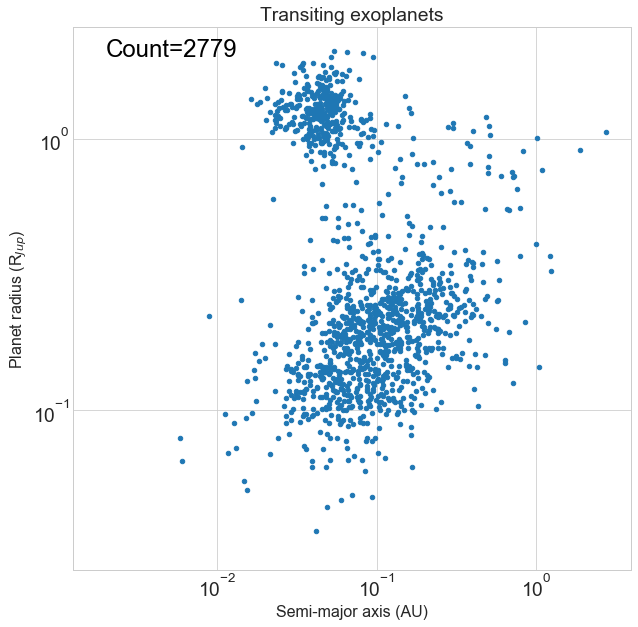
\includegraphics[width=7cm]{figures/statistics_a_vs_R.png}
\caption{Transiting exoplanets discovered to date. The diagram shows two general transiting planet populations based on radius and semi-major axis (i.e. hot Jupiter and mini Neptune). The data comes from NASA Exoplanet Archive retrieved on January 2018.}
\label{fig:stat}
\end{figure}

\paragraph{Bulk composition}
Moreover, if the planet’s mass is also known, %either via spectroscopic and radial velocity measurements, 
then combining mass with the radius determined via the transit technique yields the planet’s density which is the first step towards distinguishing between gaseous and rocky planets. 
%RV technique: 
%Radial Velocity Measurement
%The radius of the planet are directly imprinted on the transit lightcurve. Similarly, the radial velocity (RV) technique which measures the line-of-sight wobble of star due to the orbiting planet is sensitive to massive planets in short orbits around bright stars. The RV technique however provides mass information which together with radius derived from transit technique, yields the planet’s bulk density which is the first step towards distinguishing between gaseous and rocky planets. 
%Direct Imaging
%In comparison, direct detection method such as high contrast imaging which spatially resolves the planet from the star is sensitive to big, young and hence self-luminous sub-stellar objects and/or objects located far from their star such that their faint signal can be distinguished from the glare of the host star. 
Figure~\ref{fig:density} shows more than 500 exoplanets with measured mass and radius and the curves represent different (theoretical) planet  compositions ranging from pure light elements (e.g. H \& He) to dense metals (e.g. Iron). This plot demonstrates the compositional diversity that cannot be understood by studying the Solar System planets alone. Thus, studying exoplanets offers the perfect laboratory to test theories of planet formation. While density can help distinguish between gaseous and rocky exoplanets, it cannot provide information about the presence of trace elements, as well as its chemistry and dynamics. Thus, current research is focused towards detection and characterization exoplanet atmosphere because it offers the most reliable way to detect biosignatures and hence assess the planet's habitability (e.g., Burrows et al. 2014). 
\begin{figure}
\centering
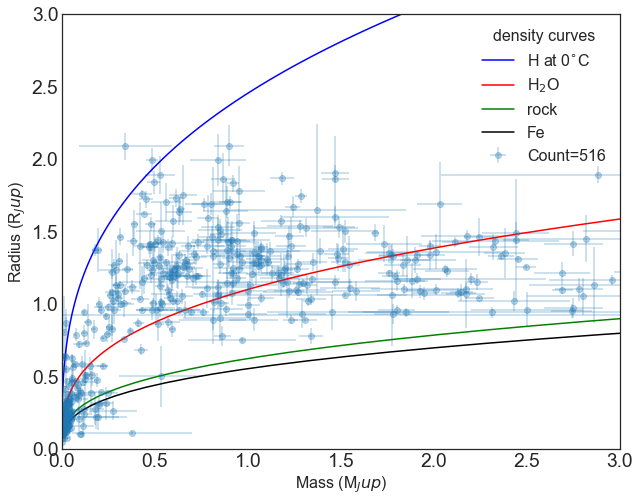
\includegraphics[width=7cm]{figures/density.png}
\caption{Compositional diversity of transiting exoplanets. More than 500 transiting exoplanets have measured mass and radius which provide constraint on their bulk density. Taking uncertainty into account, known exoplanets span a range of compositions from pure light elements (e.g. Hydrogen) to dense metals (e.g. Iron).}
\label{fig:density}
\end{figure}

%ground-based observation plays a vital role in validating and for further detailed characterization
%Although the interest in shifting towards M dwarfs
%ground-based telescope is still confined with relatively large gaseous planets 
%especially in the case of robustly detecting broad atmospheric signatures such as Rayleigh scattering with photometry
%hot Jupiters remain prime targets to accomplish this task
%Fukui+2016 demonstrated that MuSCAT can detect such atmospheric feature but for planets not currently available   
%Until the advent of TESS era and assuming its predicted discoveries come into fruition, we continue to improve transit modeling and more robust statistical modeling  
%Thus, the main targets of this thesis are hot Jupiters
%low density hot Jupiters offers the best chance to detect

%Fig.~\ref{fig:density} shows the mass-radius diagram of small exoplanets illustrating the diversity of their composition. The sparsity of objects in the diagram shows that terrestrial planets in the HZ are only beginning to present themselves. Similarly, the diagram shows the technical difficulties in obtaining reliable mass and radius measurements for solid exoplanets. The key to overcome this difficulty is to observe planets around late type stars. M-dwarfs for example have been shown to comprise 70\% of stars in the solar neighborhood (i.e. within 10 pc; Bochanski et al., 2010). Due to its proximity and frequency coupled with their smaller masses and radii, M dwarf systems hold the key to finding terrestrial planets in the habitable zone (HZ)—regions around the star where liquid water may exist and possibly life (Hart, 1979; Kasting et al., 1993). Indeed, most M dwarfs are now known to host closely-packed planetary systems characterized by a paucity of Jupiter-mass planets and the presence of multiple rocky planets, with roughly a third of these rocky M-dwarf planets orbiting within the HZ, including the three of the seven TRAPPIST-1 planets recently discovered (Gillon et al. 2017). Thus, M dwarfs have become prime targets for finding and characterizing terrestrial exoplanets. 
%The difficulty lies on the few known M dwarfs to date. 

%By now, more than 300 planets transiting their host star have been found, and much effort is being put into measuring the properties of each system. 

%\section{Transits and Occultations}
%When transiting in front of its host star, a planet blocks a fraction of the incident stellar light. The amount of blocked light relative to the original stellar light is called the transit depth. Since a set of transit depths observed at different wavelengths (called transmission spectrum) depends on atmospheric constituents, one can infer the atmospheric composition via multi-wavelength transit observations.

%\subsection{Transmission spectrum from transit observation}
%As a planet transits its parent star, some of the stellar flux passes tangentially through the planet's limb and upper atmosphere. For an extended atmosphere, the transit depth is wavelength-dependent. 

\paragraph{Exoplanet atmosphere}
During a transit, a small fraction of the starlight (e.g. 1–2\% for a typical hot Jupiter) %this can be confirmed in exoplanet plot pl_trandep
is blocked by the planet's opaque disk. On top of the disk, however, there is an optically-thin annulus (i.e. the exoplanet's upper atmosphere if present) through which incident light can be transmitted, absorbed, or scattered depending on the atmospheric properties. %Because the atmospheric opacity varies with wavelength, the apparent radius at which the planet's atmosphere becomes optically thick changes with wavelength (Seager \& Sasselov 2000; Brown et al. 2001; Hubbard et al. 2001). 

\begin{figure}
\centering
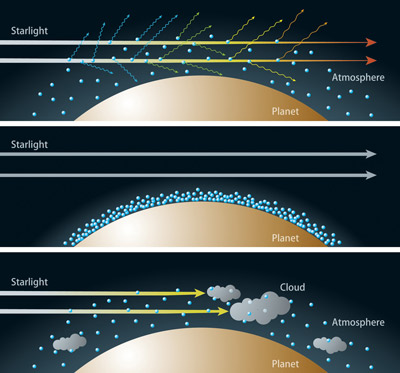
\includegraphics[width=7cm]{figures/atmosphere.jpg}
\caption{A cartoon illustrating the relationship between the composition of the atmosphere and transmitted colors of light. (credit: NAOJ)}
\label{fig:atm}
\end{figure}

If the sky has a clear, upward-extended, hydrogen-dominated atmosphere, Rayleigh scattering disperses a large portion of the blue light from the atmosphere of the host while it scatters less of the red light. As a result, a transit in blue light becomes deeper than the one in red light (see Fig.\ref{fig:atm} (top)). If the sky has a less extended, water-rich atmosphere, the effect of the Rayleigh scattering is much weaker than in a hydrogen-dominated atmosphere. In this case, transits in all colors have almost the same transit depths (see Fig.\ref{fig:atm} (b)). If the sky has aerosol\footnote{aerosol is loosely defined here as particles suspended in a gas and can refer to clouds, haze, and dust interchangeably}, most of the light cannot be transmitted through the atmosphere, even though hydrogen dominates it. As a result, transits in all colors have almost the same transit depths (see Fig.\ref{fig:atm} (c)). 

%\section{Rayleigh Scattering}
%\subsection{Theory}
%If the sky has a clear, upward-extended, hydrogen-dominated atmosphere, Rayleigh scattering disperses a large portion of the blue light from the atmosphere of the host while it scatters less of the red light. As a result, a transit in blue light becomes deeper than the one in red light.
%The transmission spectrum of a transiting planet therefore contains information about the scattering and absorption properties of the upper atmosphere near the planet’s day-night terminator.
In practice, this wavelength-dependent radius variation can be measured by multi-color photometry in which change in flux arising from rays that pass through the planet's atmosphere:
\begin{equation} 
\delta F_{\rm{transit}} = \frac{\pi(R^2-R^2_0)}{\pi R^2_s} \approx \frac{2R_0\delta R}{R^2_s}
\end{equation}
$\delta F_{\rm{transit}}$ is essentially an annulus of the atmosphere ($2\pi R_0 \delta R$), divided by the area of the stellar disk ($\pi R^2_s$). Here, the apparent radius $R=R_0+\delta R$ where $\delta R$ is the (small) deviation from the planet radius $R_0$ measured at some reference wavelength. The change in transit radius is usually some multiple of the (isothermal) scale height $H$: $\Delta R = nH$, with typical $n\sim 5$ depending on the spectral resolution and wavelength. 
The scale height, the vertical distance over which the gas pressure drops by a factor of $e$, is expressed as
\begin{equation} 
\label{eq:H}
H=\frac{kT_{eq}}{\mu g}
\end{equation}
where $k$ is the Boltzmann constant, $T_{eq}$ is the atmospheric temperature, $\mu$ is the mean molecular weight, and $g_p$ is the planetary surface gravity. Measuring $\delta F_{\rm{transit}}$ across several wavelengths constitutes the planet's transmission spectrum. 
%The mixing ratios of the absorbers and surface/cloud-top pressure, together with $\mu$ and $r_p$, are the atmospheric properties that affect (and can be inferred from) the spectrum.

%Several observations have been conducted to take the spectrum of exoplanets. Some spectra show 

\begin{comment}
\begin{figure}
\centering
\includegraphics[width=7cm]{figures/mancini.png}
\caption{Optical transmission spectrum of a hot Jupiter WASP-98 b where different models for clear (green), cloudy (yellow), hazy (blue), and best-fit (red) model are superposed to the measured optical spectrum (black data points) of the planet (Mancini et al. 2016)}
\label{fig:mancini}
\end{figure}
\end{comment}

%Additionally, multiple-band photometry of a TEP system can be used to constrain the composition of an exoplanet’s atmosphere. 
%sample sizes for is still too small to enable robust statistical investigations.
%Despite a great deal of theoretical work, the mechanism(s) by which hot Jupiters are emplaced onto misaligned orbits–and even whether an alternate mechanism, rather than tides, might actually be responsible for the trends described above–remains unclear.
%A variety of further observations are needed to distinguish among these models.

Although multi-color photometry generally does not have the power to resolve specific atoms or molecules, it is still useful to observe broad spectral features and test for the presence or absence of aerosol (e.g., Croll et al. 2011; de Mooji et al. 2012, 2013; Fukui et al. 2013, 2014; Mancini et al. 2013, 2014; Narita et al. 2013a,b; Nascimbeni et al. 2013, 2015).  

\paragraph{Aerosols in exoplanet atmosphere}
Presence of aerosol in the form of clouds and/or hazes in the exoplanet's atmosphere can be inferred based on the Rayleigh scattering signature detected in the optical wavelengths. %Any significant deviation from a flat line could mean anything between clear or cloudy atmosphere. 
Fig.~\ref{fig:atm_haze} shows a comparison of the transmission spectrum models with and without haze in the the atmosphere of a typical hot Jupiter. Between 0.5--5 $\mu$m, haze in the upper atmosphere %($P\lesssim 10^{-4}$ bar) 
causes radiation to become optically thick and prevent the molecules in the lower atmosphere %($P\gtrsim {10}^{-4}$ bar) 
such as H$_2$O, CH$_4$, and HCN from showing their absorption features. %Horizontal dotted lines represent the transit depths corresponding to the pressure levels from $1\times 10^{-6}$ bar to 1 bar for the atmosphere without haze. 
In the optical (0.3–1 $\mu$m), the spectral slope due to Rayleigh scattering by small ($\lesssim$ 0.1 $\mu$m) haze particles in the upper atmosphere can be seen. Thus, a relatively featureless spectrum in the near infrared and a large Rayleigh scattering in the optical can be used to infer the existence of haze in the atmosphere. 

\begin{figure}
\centering
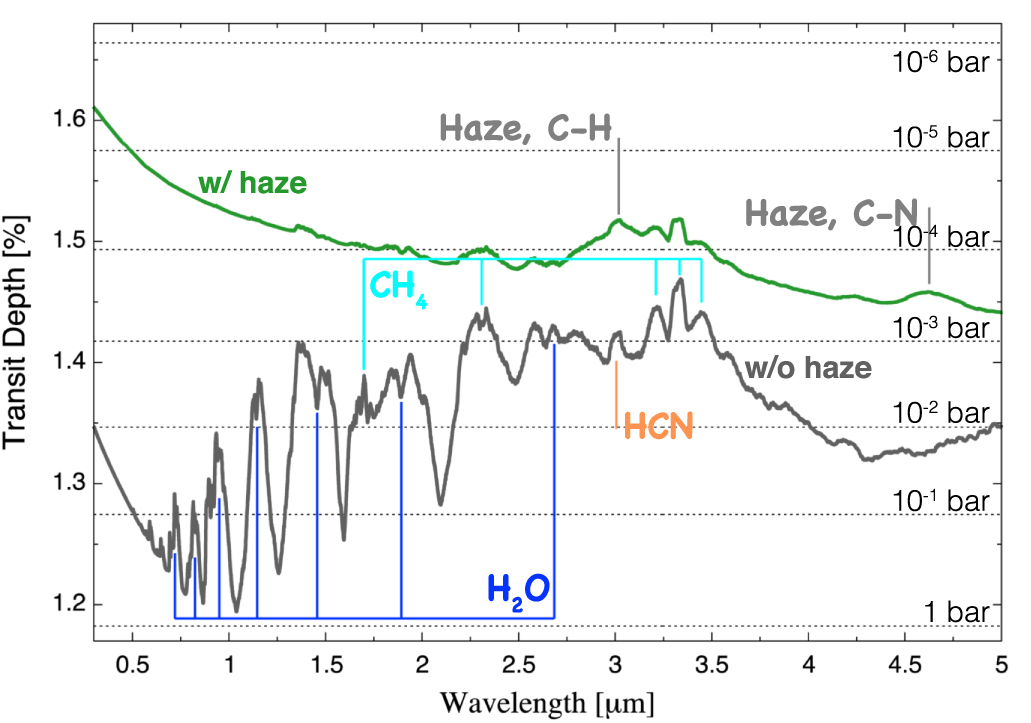
\includegraphics[width=8cm]{figures/haze_kawashima2017.jpg}
\caption{Transmission spectrum models for a clear atmosphere (black line) and  a hazy atmosphere (green line). Haze in the planet's upper atmosphere causes radiation to become optically thick and prevent the molecules in the lower atmosphere from showing their absorption features. A relatively featureless spectrum in the near infrared and a large Rayleigh scattering in the optical can be used to infer the existence of haze in the atmosphere. (credit: Fig.~9 in \cite{Kawashima2017})}
\label{fig:atm_haze}
\end{figure}



\begin{comment}
\subsection{Summary of Observation of Low Density Hot Jupiters}
%Investigation of atmospheric composition of transiting exoplanets by multi-band photometric observations with the aim of detecting variation of the planet’s radius as a function of wavelength has been conducted by a few groups recently (Southworth et al. 2012b; Mancini et al. 2013a,b,c;Nikolov et al. 2013).

So far, transit spectroscopy of exoplanets has been mainly performed on two hot Jupiters: HD209458b and HD189733b. Located at relatively close distances (47 and 19 pc, respectively), the two stars (G0V and K1-K2, respectively) have a visible magnitude V of 7.7, much brighter than the host stars of the other transiting hot Jupiters. 


%==========================================================================
\section{Observations of Low Density Hot Jupiters}
%hot Jupiters, including WASP-6b (Jordán et al. 2013; Nikolov et al. 2015) and WASP-31b (Sing et al. 2015). 

%An increase in planetary radius with decreasing wavelength in the atmosphere of the hot Jupiter HD 189733b is first reported by Pont et al. (2008) and Sing et al. (2011), based on Hubble Space Telescope (HST) Advanced Camera for Surveys and Space Telescope Imaging Spectrograph (STIS) observations, respectively. Pont et al. (2008) and Sing et al. (2011) demonstrate the effect is planetary rather than stellar, and they attribute it to the presence of Rayleigh scattering due to high-altitude hazes. 

%A few groups (Pont et al. 2008; Sing et al. 2011, 2015; de Mooij et al. 2013; Narita et al. 2013; Dragomir et al. 2015) conducted a search for the Rayleigh-scattering slope at optical wavelengths for smaller planets around.

%Narita et al. (2013) and de Mooij et al. (2013) have carried out such observations for GJ 1214b, a warm super- Earth orbiting a M dwarf, but found the transmission spectrum to be as featureless at these short wavelengths as it is at longer wavelengths (Berta et al. 2012; Fraine et al. 2013). 

%Notable examples are 55 Cnc e (Demory et al. 2011; Winn et al. 2011; V=5.95) and HD 97658b (Dragomir et al. 2013; V=7.7).  GJ 1214b (Charbonneau et al. 2009; V=14.7), GJ 436b (Gillon et al. 2007; V=10.6), and GJ 3470b (Bonfils et al. 2012; V=12.3), all of which orbit M dwarf (so smaller) stars, are such systems. This small, but growing, sample of favorable super-Earths, sub-Neptunes, and hot Neptunes continues to be the target of considerable effort to probe these planets' atmospheres via transmission spectroscopy (Seager \& Sasselov 2000; Brown 2001).

%So far, these observations often reveal featureless transmission spectra, which are interpreted as a high-mean-molecular-weight atmosphere and/or high-altitude hazes (Miller-Ricci et al. 2009; Kreidberg et al. 2014).

%These studies emphasize the importance of adequately characterizing the stellar variability and the spot properties when undertaking such analyses. 

%Fukui et al. (2016) demonstrated the ability of MuSCAT to probe atmospheric features of exoplanets larger than super-Earths (Fig. 5). Because known cool planets are too faint for ground-based telescopes, there are not enough targets to date observed with MuSCAT with sufficient precision.

%The first discovered exoplanet around a main sequence star is a hot Jupiter named 51 Peg b (\cite{Mayor1995}) thanks to its large radius and short period. 
%scale height
%Rayleigh scattering

%==========================================================================

Hot Jupiters—Jupiter-sized planets that orbit very close to the star, currently dominate spectral data of exoplanet atmospheres. A comparative study of ten hot Jupiter atmospheres reported a continuum from clear to cloudy atmospheres (Sing et al. 2016) wherein more irradiated atmospheres tend to have less clouds (Fig. 3; Heng et al. 2016). 

WASP-31b 
WASP-12b 
HAT-P-12b 
HD189733b 
WASP-6b

However, it is not known whether smaller, cooler planets follow the same trend. Although it is known that hydrocarbon haze particles can be produced via photochemical processes in low-temperature (T<1000 K) atmospheres such as that of Neptune and Uranus, empirical data is lacking to support this claim mainly due to the very few currently-known transiting low-temperature planets that are observable either on the ground or in space. However, this situation will be dramatically changed by TESS, which will detect hundreds of super-Earths/Neptunes around nearby M dwarfs (see Fig. 2). This offers MuSCAT2 a golden opportunity to follow-up new targets as soon as they become observable from the ground. Aside from confirming the new TESS candidates and refining their transit parameters, MuSCAT2 will be able to provide optical spectra in four bands that are generally useful to constrain the presence/absence and perhaps even degree of cloudiness of these cool or warm transiting exoplanets around nearby M dwarfs.


to obtain and constrain fundamental system parameters:
%==========================================================================
\end{comment}

\section{Motivation}\label{sec:followup}
%\section{Planet validation}
%follow-up observation/ validation/ detailed characterization
To confirm and characterize detected transiting systems, follow-up observations are necessary. %(see also $\S$\ref{sec:followup}). 
Generally, there are three methods for follow-up studies: (1) multi-color transit photometry used to measure any wavelength-dependent radius variation; (2) AO/lucky imaging to resolve any contaminating background stellar-mass sources; and (3) reconnaissance spectroscopy and RV measurements to measure mass limits of the companion. In this study, we focus on multi-color transit photometry. %Among the three planet validation methods, only multi-color transit photometry yields constraints on atmospheric properties of the planet. 

%Narita+2013
%Experiences have shown that broadband single-color transit photometry is not efficient to constrain an atmosphere model in the presence of starspots and the stellar variability. More effective ways to characterize atmospheres of transiting planets would be (1) simultaneous multi-color transit photometry using small-medium ground-based telescopes (e.g., Croll et al. 2011; de Mooij et al. 2012; Narita et al. 2013; Fukui et al. 2013b)

Multi-color transit photometry can eliminate false positive detections by measuring the change in the observed planet radius as a function of wavelength during the transit. For example, eclipsing binary stars, which can mimic the signal of a transiting planet, produce significant wavelength-dependent radius variation caused by stellar photosphere whereas a true planet produces weaker variation due to stellar limb darkening and its atmosphere if present. 
%One such survey is the multi-color Transiting (MuSCAT) project (Narita et al. 2014) which has been carrying out follow-up observations for 3 years now.
%Discovery of transiting exoplanet systems are mostly conducted by dedicated surveys (e.g. HAT-net). Follow-up observations are important to confirm the planetary nature of the transit signal and improve the properties of the system.
%Follow-up transit photometry can also improve the transit ephemeris which is useful for precise transit prediction in future observations. Checking for transit-timing variations (TTV) in several epochs can provide constraints on the existence and possibly mass of non-transiting companion(s) in the system. 
Precise measurement of transit depths (i.e. planet radius) at multiple wavelengths %(called transmission spectrum) 
provide independent constraint on atmospheric property. With an estimated planetary temperature and gravity, the detection of a Rayleigh scattering slope yields the atmospheric scale height which can then be used to estimate the mean molecular mass for general atmospheres independently of other atmospheric properties (\cite{Benneke2012}). 
%The wavelength dependence of transit depth can also be used to characterize the atmospheres. In particular, the linear slope of the Rayleigh scattering signature %or the shapes of individual features
%provide constraints on the atmosphere scale height 
%first detection of atmosphere (Charbonneau 2002)
Moreover, detection of Rayleigh scattering slope in the optical usually by ground-based facilities is complementary to near-infrared transmission spectrum obtained usually using space telescopes. For example, GJ 3470b has been found to exhibit a flat transmission in the infrared which is interpreted as either due to a clear atmosphere with high-mean-molecular-weight or high-altitude  hazes (\cite{Kriedberg2014}; See also Fig.~\ref{fig:atm_haze}). Detection of Rayleigh scattering in the optical by \cite{Dragomir2015} help break such degeneracy by favoring an atmosphere model with hydrogen/helium-dominated atmosphere covered by hazes which obscure absorption features in the IR and hazes which give rise to scattering in the visible. This demonstrates the possibility to characterize the atmospheres of exoplanets using shorter-wavelength measurements even when their IR transmission spectra are featureless.
%We find that the most plausible scenario is a hydrogen/helium-dominated atmosphere covered by clouds which obscure absorption features in the infrared and hazes which give rise to scattering in the visible.

Most detections of Rayleigh scattering have been found in giant exoplanets with low densities since Rayleigh scattering signal is larger for planets with larger scale heights (See Eq.~\ref{eq:H}). Small planets transiting somewhat fainter stars are also accessible to existing facilities if their transits are deeper than the order of 0.1\% for a system with a smaller host star and/or a larger planet. Despite the large numbers of known or candidate planets, and despite the ubiquity of planets around small late-type stars, the host stars of most systems known to date are too faint for the detection and characterization of exoplanet atmospheres especially using ground-based telescopes.
This problem is compounded by the fact that light curves of planetary transits often contain deviations from a simple transit shape, and it is generally difficult to differentiate between anomalies of astrophysical nature (e.g. starspots) and correlated noise due to instrumental or atmospheric effects.

%While it is important to enlarge the number of detected planets, it is also vital to accurately measure the main physical properties of each planetary system used in statistical analysis.

Recent observations of transiting hot Jupiters using the Space Telescope Imaging Spectrograph (STIS) and Wide Field Camera 3 (WFC3) on the Hubble Space Telescope (HST) have revealed a variety of atmospheric characteristics. Most notably, the 10 hot Jupiters reported in Sing et al. (2016) 
%(for additional details of observations, see Huitson et al. 2013; Line et al. 2013a; Mandell et al. 2013; Pont et al. 2013; Sing et al. 2013, 2015; Wakeford et al. 2013; McCullough et al. 2014; Nikolov et al. 2014, 2015) 
indicate a variety of atmospheres, interpreted as a continuum of clear to hazy conditions. The diversity of these results emphasizes the need to increase the current pool of studied gas giant atmospheres to better understand the physical properties of low density hot Jupiters and the parameters governing the presence or absence of hazes. 

%Although it is known that hydrocarbon haze particles can be produced via photochemical processes in low-temperature (T<1000 K) atmospheres such as that of Neptune and Uranus, empirical data is lacking to support this claim mainly due to the very few currently-known transiting low-temperature planets that are observable either on the ground or in space. However, this situation will be dramatically changed by TESS, which will detect hundreds of super-Earths/Neptunes around nearby M dwarfs (see Fig. 2). This offers MuSCAT2 a golden opportunity to follow-up new targets as soon as they become observable from the ground. Aside from confirming the new TESS candidates and refining their transit parameters, MuSCAT2 will be able to provide optical spectra in four bands that are generally useful to constrain the presence/absence and perhaps even degree of cloudiness of these cool or warm transiting exoplanets around nearby M dwarfs.

%Thus, factors motivate additional observations in this wavelength regime.
Motivated by this need, we carry out simultaneous, multi-color transit photometry of low-density hot Jupiters with the goal of refining the physical parameters of such systems and searching for broad atmospheric features using a dedicated instrument discussed in the next section.

\section{OAO/MuSCAT\label{sec:muscat}}
%%%%%%%%%%%%%%%%%%%%%%%%%%%%MuSCAT%%%%%%%%%%%%%%%%%%%%%%%%%%%%%%%%%%%
%We report a development of a multi-color simultaneous camera for the 188-cm telescope at Okayama Astrophysical Observatory in Japan. The instrument, named MuSCAT (multi-color Simultaneous Camera for studying Atmospheres of Transiting exoplanets), has a capability of three-color simultaneous imaging in optical wavelengths where CCDs are sensitive. MuSCAT is equipped with three 1024 × 1024 pixel CCDs which can be controlled independently. The three CCDs detect lights in g2′ (400 to 550 nm), r2′ (550 to 700 nm), and zs,2 (820 to 920 nm) bands using Astrodon Photometrics Generation 2 Sloan filters. The field of view of MuSCAT is 6.1×6.1  arc min2 with the pixel scale of 0.358  arc sec/pixel. The principal purpose of MuSCAT is to perform high-precision multi-color transit photometry. For this purpose, MuSCAT has the capability of self-autoguiding which enables it to fix the positions of stellar images within ∼1 pixel. We demonstrate relative photometric precisions of 0.101%, 0.074%, and 0.076% in g2′, r2′, and zs,2 bands, respectively, for GJ 436 (magnitudes in g′=11.81, r′=10.08, and z′=8.66) with 30-s exposures.

For this study, we used the multi-color Simultaneous Camera for studying Atmospheres of Transiting exoplanets (MuSCAT), which is an optical three-band instrument that was recently developed for the 188 cm telescope at the Okayama Astrophysical Observatory (OAO; \cite{Narita2015a}). 
MuSCAT has three three CCD cameras equipped with the Sloan $g'_2$, $r'_2$, and $z_{s,2}$ filters (hereafter g-, r-, z-bands), which can obtain images in three bands simultaneously (\cite{Narita2015a}). Each CCD has pixel scale of 1".5 pixel$^{-1}$ and FOV of 5.6' $\times$ 5.6' . Technical specifications are summarized in Table~\ref{tab:muscat}.
MuSCAT has demonstrated its capability to achieve precision photometry with nominal error of rms(5-min)~0.02 for Vmag=10 star as in the case of HAT-P-14b (\cite{{Fukui}2016a}).
MuSCAT has also been successful in confirming and characterizing transiting exoplanets ranging from hot Neptunes (e.g., \cite{Narita2017}) to super-Earths in the habitable-zone (\cite{Fukui2016b}). 

\begin{table}
\centering
\caption{OAO/MuSCAT basic specification.} \label{tab:muscat}
\begin{tabular}{lll} \hline
             &Value      \\ 
\hline
Primary mirror & 1.88 m \\
Location       & 34$^{\circ}$34'37"N 133$^{\circ}$35'38" E, 372m \\
Filters  \multirow{3}{*}{} & g'$_2$: 400-550nm \\
                           & r'$_2$: 550-700nm \\
                           & z$_{s,2}$: 820-920nm \\
FOV    & 6.1'x 6.1' \\
Pixel scale & 0.36'' / pix \\ 
\hline
\end{tabular}
\end{table}

\begin{figure}
\centering
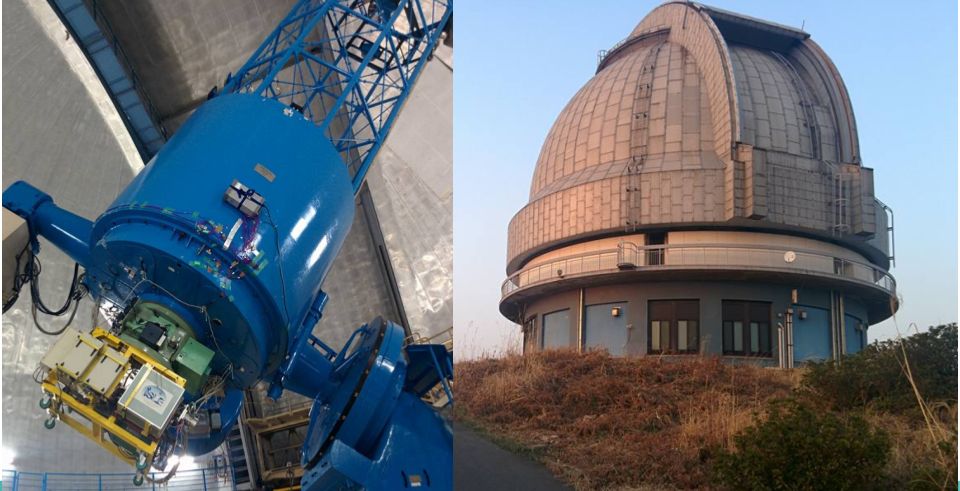
\includegraphics[width=7cm]{figures/oao-muscat.png}
\caption{OAO/MuSCAT}
\label{fig:muscat}
\end{figure}

%detecting a tiny (0.06%) transit of the K2 habitable-zone super-Earth K2-3d (Fukui et al. 2016b). It has also been used for validating transiting planetary candidates discovered from K2, as a part of the ESPRINT/KESPRINT collaboration (Hirano et al. 2016a, Narita et al. 2017).

%Moreover, Cabrera et al. (2017) demonstrated the importance of independent confirmation of planetary candidates after demoting the statuses of previously the validated planets K2-78b, K2-82b, and K2-92b into eclipsing binaries. % https://arxiv.org/pdf/1707.08007.pdf

%==========================================================================
\section{Targets: Hot Jupiters}\label{sec:targets}
We consider three targets for this thesis: HAT-P-44, HAT-P-12, and WASP-21 which were observed as part of on-going follow-up observation of transiting exoplanets with MuSCAT. 
%The main reason for selecting this system for a pilot observation is that a good comparison star with a similar brightness to the host star (V=9.6) exists within the FOV (HIP 84832; separated from HAT-P-14 by 4 4), offering a good opportunity to achieve a high photometric precision. Stars
These targets are chosen based on the planets' relatively low mean densities and hence large scale heights which therefore increases their likelihood to have a gaseous atmosphere on top of a solid surface. The expected scale height is computed using Eq. \ref{eq:H} assuming $\mu$=2.3 for H-H2 dominated atmospheres. %strongly irradiated and inflated giant planets
The stars' and planets' properties are summarized in Table~\ref{tab:params} and the observation log is summarized in Table~\ref{tab:obs}. Unless a more reliable measurement is available, the values are taken from discovery papers: HAT-P-44: \cite{Hartmann2014}; HAT-P-12: \cite{Hartmann2009}; WASP-21: \cite{Bouchy2010}. We summarize each system as follows.

%Short summary of our targets
%HAT-P-12: http://exoplanet.eu/catalog/HAT-P-12_b/
%ApJ, 834:50 (15pp), 2017 January 1
\paragraph{HAT-P-12b}
%HAT-P-14b (aka WASP-27b), a hot Jupiter orbiting a bright (V=10.1) F-type star in a retrograde and slightly eccentric (e= 0.1) orbit with the period of 4.63 days (Torres et al. 2010; Simpson et al. 2011; Winn et al. 2011). So far only one photometric follow up observation has been reported after the discoveries (Nascimbeni et al. 2011), leaving room for further photometric follow-ups to search for such as TTVs, TDVs, and transit- depth variations.
HAT-P-12b was detected with the HAT-5 telescope of the Hungarian-made Automated Telescope Network %(Bakos et al. 2004) 
in 2006. \cite{Hartmann2009} %Hartman et al. (2009) 
conducted follow-up photometry of four transits together with
spectroscopic observations and reported that the planet has a mass smaller than Saturn's and radius similar to Jupiter's, respectively, in a 3.2 day circular orbit around a fairly bright (m$_V$=12.8) K4-type star. 
%Its host star is a K4 dwarf (V = 12.8) with MA = 0.73 ± 0.02 M, RA = 0.70+0.02 −0.01 R.
%Since HAT-P-12b is one of the lowest-density planets orbiting metal-poor host stars, the physical properties of the system are important for irradiation models.
%HAT-P-12 b is also a low-surface gravity ($g_p$=5.6 ms$^-2$) % 0.295 ± 0.025 g cm–3
%\cite{Lee2012} reported three more follow-up transit observations to improve the properties of the system  using empirical calibrations from eclipsing binary stars and stellar evolutionary models. 
HAT-P-12b has many interesting properties. \cite{Hartmann2009} noted its unusually large scale height (615.6 km) which is at least an order of magnitude larger than Saturn's. It is also one of the lowest-density ($\sim$0.32 g cm$^{-3}$) planets with a fairly warm temperature $T_{eq}$=963 K %for a hot Jupiter  
orbiting metal-poor host stars. Due to these reasons, HAT-P-12b has been the subject of extensive follow-up observations both from ground and space (e.g. \cite{Lee2012}; \cite{Todorov2013}; \cite{Sing2016}). %and atmospheric modeling using its spectrum (e.g. \cite{Todorov2013}; \cite{Line2013}; \cite{Stevenson2016}). %high albedo >0.8 accdg to Barstow+17

%A LOW-DENSITY SUB-SATURN MASS PLANET TRANSITING A METAL-POOR K DWARF
In particular, HAT-P-12b reported \cite{Line2013} its transmission spectrum obtained using the Hubble Space Telescope's (HST) WFC3 instrument which showed lack of water absorption feature expected for a hydrogen-dominated atmosphere, favoring a model with high-altitude clouds. Subsequent observations using HST/STIS in the optical and Spitzer/IRAC in the infrared by \cite{Sing2016} reported it to be one of the 10 hot Jupiter samples with strong optical scattering slopes. More recently, \cite{Barstow2017} confirmed that HAT-P-12b's transmission spectrum is consistent with the presence of Rayleigh scattering due to atmospheric aerosol/ haze. 

Given a wealth of information, HAT-P-12b is included in our sample as a test case for verifying the results of our transit analysis.
%extending to low atmospheric pressures (below 0.1 mbar).
% In general, planets with equilibrium temperatures between 1300 and 1700 K are best represented by deeper, gray cloud layers, whereas cooler or hotter planets are better fit using high Rayleigh scattering aerosol. 
%In concordance with previous studies, we find that vertically homogeneous, small particle (<0.1 µm) clouds are best at producing strong Rayleigh scattering signatures, but only if iron-bearing cloud species are neglected. (Molliere+2017)

\paragraph{HAT-44}
%For HAT-P-44 we find that the preferred model, based on the estimated Bayes Factor, consists of two planets, the outer one on an eccentric orbit. This model includes: the transiting planet HAT-P-44b with a period of P = 4.301219 ± 0.000019 days, a mass of M p = 0.352 ± 0.029 M J , and an eccentricity of e = 0.044 ± 0.052; an outer planet HAT-P-44c with a period of P = 872.2 ± 1.7 days, a minimum mass of M p sin i = 4.0 +1.4 −0.8 M J , and an eccentricity of e = 0.494 ± 0.081. We adopt the model with the long period and high eccentricity for the outer component because it has the highest Bayes factor.
%\cite{Hartmann2014} report the discovery of HAT-P-44b identified using the HATNet telescopes, and then confirmed through follow-up observations with a variety of ground-based facilities. 
HAT-P-44b was detected with the HAT-5 telescope of the Hungarian-made Automated Telescope Network %(Bakos et al. 2004) 
in 2006. \cite{Hartmann2014} %Hartman et al. (2009) 
conducted follow-up photometry of five transits from 2010-2011 together with two spectroscopic observations and reported that the planet has a mass and radius % M=0.35,  R=1.24 
both slightly larger than Saturn and Jupiter, respectively, in a slightly eccentric (e=0.04) %0.044±0.052) 
4.3-day orbit around a relatively faint (m$_V$=13.2) G-type star.
%mass of 0.35 $M_J$, and radius of 1.24 R$_J$ yielding a density of 0.23 $\pm$ 0.04 (\cite{Hartmann2014}). 
Similar to HAT-P-12b, HAT-P-44b is a bloated planet with similar density of $\sim$0.23 g cm$^{-3}$ (\cite{Hartmann2014}) with a large scale height of $\sim$ 708 km.

Follow-up RV observation reveal significant systematic variations in its residual radial velocities, indicating the presence of an outer non-transiting companion. Combined RV+transit modeling indicate that HAT-P-44 consists of two planets, including the transiting component, with the outer planet having a period of 872 days, eccentricity of 0.494 $\pm$ 0.081, and a minimum mass of 4.0 M$_J$.
%In this regard, it is important to check whether transit timing variation can be detected from out photometric observation. (PERIOD TOO LONG!)

So far only few photometric follow up observations have been reported for HAT-P-44b which are included in the discovery paper (\cite{Hartmann2014}), leaving room for further photometric follow-ups to search for possible transit-timing variation (TTV), transit duration variation (TDV), and transit-radius variation (TRV). The follow-up photometric observations of HAT-P-44b was previously conducted using $r$ and $i$-bands but only a single Rp/Rs measurement are reported. Hence, this study will report the first ever search for such variations.

%The preferred model has an associated jitter of 10.7 ± 2.0 m s −1 and a χ 2 per degree of freedom, including this jitter, of 1.67. Based on Equation (1), one expects only 1.2\% of stars like HAT-P-44 to have jitter values 10.7 m s −1 thus the excess scatter in the RV residuals from the best-fit two-planet model suggests that perhaps more than two planets are present in this system, though we cannot conclusively detect any additional planets from the data currently available.

\paragraph{WASP-21}
%https://exoplanetarchive.ipac.caltech.edu/cgi-bin/DisplayOverview/nph-DisplayOverview?objname=WASP-21+b&type=CONFIRMED_PLANET
WASP-21b was detected with the SuperWASP-North telescope
in 2006. \cite{Bouchy2010} %Hartman et al. (2009) 
conducted follow-up photometry of five transits in 2008 together with eight spectroscopic observations and reported that the planet has a mass and radius % M=0.35,  R=1.24 
similar to Saturn and Jupiter, respectively, in a circular 4.3-day circular orbit around a relatively bright (m$_V$=11.6) G-type star.

%Bouchy et al. (2010) discovered this planetary system, and obtained its physical properties using their version of the dEB constraint. They obtained adaptive-optics imaging which show no faint stars contaminating the flux from the system. The interest in WASP-21 lies in its Saturn-mass planet (Mb = 0.295 ± 0.030MJup) and the metallicity which is the lowest known for a TEP host star (? Fe H ? = −0.46±0.11). Barros et al. (2011) analysed LT/RISE observations covering three transits, of which the firstwas originally presented in the discovery paper (Bouchyet al. 2010).They used theY2 models to provide their additional constraint, yielding significant differences compared to those found by Bouchy et al. (2010): MA = 0.86 ± 0.04M?versus 1.01±0.03M?,andMb=0.27±0.01M?versus 0.300±0.011M?.WASP-21

Similar to HAT-P-12b, WASP-21b is a bloated planet with similar density of $\sim$0.32 g cm$^{-3}$ (\cite{Bouchy2010}) around a metal-poor host. 

\cite{Barros2011} and \cite{Ciceri2013} found lower values for the mass and the density of the planet (by 1.0 and 1.4$\sigma$ respectively) with respect to those found in the discovery paper. In either case, the planet has a scale height of $\sim$ 900 km, the largest among our sample.%, and also reported no indication of TTV. 
%However, in a later study Barros et al. (2011a) found the G3V star to be in the process of moving off the main sequence. Thus, we included further observations of WASP21b planetary transits to improve the knowledge on this system.
%photometric follow-up and stellar density modeling from transit light curve by Barros 2011 report a stellar mass of 0.86 ± 0.04 M⊙, which is significantly lower than previously reported (1.01 ± 0.03 M⊙). Consequently, we find a lower planetary mass of 0.27 ± 0.01 MJup. 
As in the previous analyses, \cite{Barros2011}, \cite{Ciceri2013}, \cite{Seelinger2015} found no trend or sinusoidal variation in the system parameters.

WASP-21b was previously conducted using $r$ and $i$-bands but only a single Rp/Rs measurement are reported. Hence, this study will report the first ever search for such variations.

\begin{comment}
%Sensitivity to atmospheric feature
\paragraph{Achievable Measurement Error of Rp/Rs with MuSCAT}
%chapter 4.3 in 
\cite{Fukui2016a} simulated the achievable measurement error of Rp/Rs with MuSCAT. Three types of planet were considered: (1) the V = 10 F-dwarf HAT-P-14, (2) the nearby (38 pc) K-dwarf HAT-P-11 (Bakos et al. 2010), and (3) the nearby (14 pc) M-dwarf GJ1214 (Charbonneau et al. 2009). 

When a planet has an atmosphere with no thick clouds, $R_p/R_s$ can vary with wavelength by up to several $\times H/R_s$.
Therefore, if $\sigma_{Rp/Rs}$ is comparable to or smaller than the expected value of $H/R_s$, then it can roughly be considered that the measurement is sensitive to the atmosphere.
 
Given $T_{eq}$ and $g_p$ and assuming $\mu$=2.3, we can use Eq.~\ref{eq:H} to estimate the expected atmospheric scale height of our targets. 
Then, we can compute for the expected %$\sigma_{Rp/Rs}$ 
rms by assuming that the achievable precision for our targets will ideally follow the Poisson distribution. In the best case, the highest photometric precision achieved using MuSCAT is typically $\sim$0.028\% for HAT-P-14 with 5-minute binning (Vmag=10; \cite{Fukui2016a}). Since 
\begin{align*}
m_1-m_2 &= -2.5\log_{10}(f_1/f_2)\\
\rightarrow \frac{f_1}{f_2} &= 10^{\Big(\frac{m_2-m_1}{2.5}\Big)}\\
%\frac{f_1}{f_2} &= 10^{\Big(\frac{13.2-10}{2.5}\Big)} = 19.9
%\frac{f_1}{f_2} &= 10^{\Big(\frac{12.8-10}{2.5}\Big)} = 13.1
%\frac{f_1}{f_2} &= 10^{\Big(\frac{11.6-10}{2.5}\Big)} = 4.36
\end{align*}
%The photometric noise/ uncertainty goes with . Thus, the increase in the expected noise should be
and Poisson noise decreases by a factor $f=\sqrt{f_1/f_2}$ for our fainter targets, then $f$=4.47, 3.63, and 2.08 and hence $\sigma_{Rp/Rs}$=0.125, 0.101, 0.058 for HAT-P-44 (Vmag=13.1), HAT-P-12 (Vmag=12.8), and WASP-21 (Vmag=11.6), respectively. %The residual rms for g-band with 5 minute binning is 0.23\%, compared to Fukui-san's 0.028\%; an order of magnitude difference. We have to reduce the rms of the residual by a factor of 5 to match the photometric precisison expected for a Vmag=13 star.


% The right vertical axis of Figure 6 shows a scale in the unit of the expected scale height, assuming an isothermal atmosphere with the equilibrium temperature of $T_{eq}$=1624 K (Southworth 2012) and a solar abundance with $\mu$ = 2.35g. The 1$\sigma$ uncertainties of the measured Rp/Rs is the level of ∼10–20 times as large as one scale height.
\end{comment}

\begin{table}
\centering
\caption{Stellar and planetary parameters of our targets.}
\label{tab:params}
\begin{tabular}{lllll} \hline
          &HAT-P-44      &HAT-P-12        &WASP-21   \\ \hline
$R_s (R_{\odot})$     &0.949$^{+0.08}_{-0.037}$&0.701$^{+0.017}_{-0.012}$ & 1.060 $\pm$ 0.04 \\
$M_s (M_{\odot})$    &0.942$\pm$0.041   &0.730 $\pm$ 0.018 &1.010 $\pm$ 0.03 \\ 
SpT  & K & K4  & G3V \\
$V_{mag}$ &13.2              &12.8            &11.6               \\
age (Gyr) &7.5$\pm$3.6       &2.5$\pm$2.0     &12$\pm$5           \\ \hline
 &HAT-P-44b      &HAT-P-12b        &WASP-21b    \\ \hline
P (d) & 4.301219 $\pm$ 0.000019  & 3.21306 $\pm$ 0.000002    &  4.322482 $\pm$ 0.000024 \\
$R_p (R_{\rm{Jup}})$&      1.242$\pm$0.106  & 0.959$\pm$0.029& 1.07$\pm$0.06 \\
$M_p  (M_{\rm{Jup}})$ &   0.352$\pm$0.029   & 0.211$\pm$0.012 & 0.300$\pm$0.011 \\
$\bar \rho$  (g cm$^{-3}$) &  0.23$\pm$0.04   &0.3192$\pm$0.0160   & 0.32$\pm$0.07    \\ % 0.295 ± 0.025 Hartmann+09
$g$  (m$s^{-2}$) & 5.62$\pm$0.01   & 5.62$\pm$0.01 & 5.07$\pm$0.035 \\ 
%logg (cgs) 2.75 ± 0.03 Hartmann+09 
$T_{eq}$  (K) & 1108$^{+51}_{-32}$   & 963$\pm$16   & 1340$\pm$32  \\
$H$ (km) & 708.2 & 615.6 & 950.0 \\
\hline
\end{tabular}
\end{table}

\section{Contents}
In this thesis, new observations for low density hot Jupiters including HAT-P-12b, HAT-P-44b, and WASP-21b in search for TTV, TDV, and TRV are reported. % and their atmosphere models. 
The rest of the paper is organized as follows. Chapter $\S$ \ref{sec:obs} summarize the observations and methods of data reduction. Chapter $\S$ \ref{sec:results} describes the analyses of new transit light curves %and stellar variability. 
$\S$ \ref{sec:discussion} presents the results of the above analyses and discusses the implications. Finally, this thesis is summarized Chapter in $\S$ \ref{sec:summary}.
%---Observation and Data Reduction
\chapter{Observation and Data Reduction\label{sec:obs}}
We observed full single transit of each of our target with the OAO/MuSCAT (see $\S$\ref{sec:muscat} for technical details) between 2016/08  and 2017/04. The image position was selected such that the target and many comparison stars were imaged together within the FOV. %among which we chose GSC 03465-00123 (V= 13.2).
%Due to the uncertain ephemeris, propagated error since last observation 3 years ago 
Whenever possible, we started the observation at least $\sim$1 hour before/after the ingress/egress to cover the full transit and obtian long baseline. The sky was perfectly clear with no moon visible during the observations. %The condition was photometric through the observations. 
The g-,r-, and z-bands images were taken with exposure times adjusted such that all stars have value counts within linearity regime of the detector, yielding different number of raw frames for each band. The typical size of the PSF was $\sim$ 11 pixels ($\sim$4") in radius.
%The exposure time was set to XX s and the dead time (including the CCD readout time of XX s and other setup times) was about XX s (duty cycle of XX\%). 
The telescope auto-guider managed to keep the centroid on the three detectors with %standard deviation 
median value of less than 2 pixels in both X and Y directions. The observation details are summarized in Table~\ref{tab:obs}.

\section{Standard Reduction}
%%%basic reduction: dark, flat, bias, linearity correction 
Primary data reduction, including bias subtraction and flat fielding, and aperture photometry was carried out with a customized pipeline by \cite{Fukui2011}. 
%The raw images were dark-subtracted and flat-fielded in a standard manner. 
To create the flat field, we median combined 50 dome flat images for each band that were obtained on the observing night. Note that we convert the time stamps, which is recorded in the FITS headers in units of Modified Julian Day (MJD) based on Coordinated Universal Time (UTC), to Barycentric Julian Day (BJD) based on Barycentric Dynamical Time (TDB) i.e. BJD$_{\rm{TDB}}$ system using the algorithm by \cite{Eastman2010}. 
%Corrections to the barycentre are more precise than the heliocentre, because the barycenter is a fixed point where gravity is constant. For maximum accuracy you want to have your barycentric corrected times in a timescale that has always ticked at a uniform rate, and ideally one whose tick rate is related to the rate that a clock would tick at the barycentre. For this reason, barycentric corrected times normally use the TDB timescale:
%http://astroutils.astronomy.ohio-state.edu/time/

\begin{table}
\centering
\caption{Observation log of each of our targets and results of aperture photometry.}
\label{tab:obs}
\begin{tabular}{lllll} \hline
                                       &HAT-P-44      &HAT-P-12        &WASP-21       \\ \hline
Observation calendar (UT)    & 2017/02/15  & 2017/04/29  & 2016/08/12\\
%comparison stars & & & & \\
exposure times (s) &60,30,60 & 40,20,50 & 50,20,50 \\
no. of data images & 376,703,376 & 349,623,277 & 483,1072,465 \\
$\sigma_{dx}$ (pix)& 0.95, 0.40, 0.64& 0.57, 0.37, 0.30 & 0.97, 0.77, 0.71 \\
$\sigma_{dy}$ (pix)& 0.50, 0.35, 0.51& 0.81, 0.39, 0.31 & 1.21, 0.62, 0.45 \\ \hline
aperture radius (pix) & 11 & 18 & 11 \\
no. of data points & 376,703,374 & 349,623,277 & 483,1072,465 \\
\hline
\end{tabular}
\end{table}

%n high-speed (2 MHz) readout mode, while the  band images were taken with the exposure time of 30 s in low-seed (100 kHz)readout mode\footnote{The reason for using the low-speed readout mode was that the CCD camera for $z_{s,2}$ band produced uncorrectable systematic noises only in the high-speed readout mode. The camera was repaired after the observation, and the problem has been fixed.}, resulting in the observing cadences of 14 s, 14 s, and 43 s for the $g'_2$- and $r'_2$ and $z_{s,2}$ band, respectively. 

\section{Aperture Photometry}\label{sec:apphot}
After the raw images were processed by performing standard over-scan correction, de-biasing, and flat-fielding (see $\S$\ref{sec:obs}), we perform aperture photometry using a customized code detailed in \cite{Fukui2011}. This custom pipeline also calculates the photometric error, including photon noise, detector noise, and scintillation noise, used as initial estimate of uncertainties in transit modeling. We summarize the steps in aperture photometry as follows.

First, we create several trial light curves using different aperture sizes and combinations of comparison stars for each observation. For the comparison stars, we select such stars that are neither saturated, nor variable. 
The aperture radius was chosen to give the smallest scatter in the flux outside of the transits, and was generally \textbf{9 to 15} pixels. %\textbf{
The reference flux was obtained by summing the flux of the comparison stars. The flux of the target star was then divided by this reference signal to produce a time series of relative flux. Each time series was normalized to have unit flux outside of the transit. After excluding obvious outliers (>50-sigma from the median), the number of data points used in the analysis in each data set is summarized in Table~\ref{tab:obs}.
%We then check the all trial light curves by eye and eliminate obviously poor-quality ones.

%%%aperture optimization
Second, in order to select the most appropriate light curve for each observation and its baseline correction model for OOT phase, we adopt the BIC for our analyses. We fit the trial light curves with an analytic transit light curve model and various baseline models simultaneously (see $\S$ \ref{sec:sysmodel}). 

%To determine the optimal apertures to use in our analysis, we generate and inspect the $\beta$ and $\sigma$ diagnostics. %plotted in Fig.~\ref{fig:}. 
%We find that the minimum red noise aperture (\textbf{XX} pixel) is frequently consistent with the minimum white noise aperture to within a few tenths of a pixel (\textbf{XX} pixel).

\section{Light Curve Modeling: Bayesian Framework}
%intro to bayesian inference
%http://iopscience.iop.org/article/10.1086/500802/pdf
A transit light curve is basically composed of two components: transit and systematics. We follow Bayesian framework (e.g. \cite{Parviainen2017}; \cite{Diaz2017}) in modeling both transit and systematics simultaneously in three MuSCAT bands for each data set. %The goal is to estimate the posterior probability distribution (as opposed to a single point estimate) of the model parameters using the Bayes' Theorem.
In Bayesian modeling, we do not get a single estimate for our model parameters as we would with maximum likelihood estimation. Instead, we get a complete posterior distribution for each model parameter, which quantifies how likely different values are for that model parameter. For example, with few data points our estimation uncertainty will be high reflected by a wide posterior distribution. As we gather more data, our uncertainty about the model parameters will decrease and we will get an increasingly narrower posterior distribution. There are many more benefits to the Bayesian approach, such as the ability to incorporate prior knowledge.

\paragraph{Bayes' Theorem}
The posterior probability density given a parameter vector $\theta$ and observational data $D$ is described by the Bayes' theorem as
\begin{align}
P(\theta|D)&=\frac{\Pi(\theta) \times \mathcal{L}(D|\theta)}{M(D)} \\
& \propto \Pi(\theta) \times \mathcal{L}(D|\theta)
%\rm{Posterior \propto Prior \times Likelihood}
\end{align}
where $\Pi(\theta)$ is the prior probability of $\theta$, $\mathcal{L}(D|\theta)$ is the likelihood of the data given $\theta$, and $M(D|M)$ is a normalizing factor also called the marginal. Since we use Markov Chain Monte Carlo algorithm to sample the posterior distribution (see $\S$ \ref{sec:MCMC}), the marginal can be ignored and so the Bayes' theorem can be simplified as given above.

\paragraph{Model Likelihood}% of Transit \& Systematics Model}
Assuming that the parameters in our model are independent, identically distributed (iid) random variables, we can expect that the residual follows a Gaussian distribution:
\begin{equation}
\label{eq:likelihood}
\mathcal{L}(D|\theta) = N(\mu,\sigma) = \frac{1}{\sqrt{2\pi \sigma^2}} \exp \Big(-\frac{(x-\mu)^2}{2\sigma^2} \Big)
\end{equation}
where $N(\mu,\sigma)$ is the normal distribution with mean model $\mu$ and standard deviation $\sigma$. Here $\mu$ is the transit model, $x$ is data divided by the systematics model, and $\sigma$ is the measured photometric uncertainty.

The likelihood is a product of individual observation probabilities, and has the unfortunate tendency to end up being either very small or very big. To avoid computational overhead, it is better to work with log probabilities instead, so that
\begin{align}
\ln \mathcal{L}(D|\theta)& = \ln\Big[(2\pi\sigma^2)^{-\frac{1}{2}}\Big] +\ln \Big[\exp\Big(-\frac{(x-\mu)^2}{2\sigma^2}\Big)\Big] \\
& = -\frac{1}{2}\ln(2\pi) -\frac{1}{2}\ln \sigma^2 -\frac{(x-\mu)^2}{2\sigma^2} \\
&= -\frac{1}{2}\Big[\ln(2\pi) +2\ln\sigma +\Big(\frac{x-\mu}{\sigma}\Big)^2\Big]
\label{eq:loglikelihood}
\end{align}
%where we can drop constant terms since the MCMC samplers only require something proportional to $\ln{P(\theta)}$. 

\subsection{Transit Modeling}\label{sec:transitmodel}
We begin by modeling the light curves in flux scale using a combination of in-transit and out-of-transit (OOT) models, described by
\begin{equation}\label{eq:lc}
F_{rel}=F_{out}\times F_{in} \\
\end{equation}
where $F_{rel}$ is the relative flux (raw flux of target star divided by flux of comparison star obtained from relative photometry), $F_{in}$ is the in-transit model, and $F_{out}$ is the OOT model including the systematics.
%We fit the light curve with the analytic model of the form $F_{\rm{white}}(t) = S_{\rm{white}}(t)\times T_{\rm{white}}(t)$, where $S_{\rm{white}}$ is a systematics model and $T_{\rm{white}}$ is a transit model in flux scale.

There are several analytic transit models but the $de$-$facto$ standard are the ones by \cite{MandelAgol2002} and \cite{Gimenez2006}. We adapt the former for this study. The transit parameters in the Mandel-Agol model are:
\begin{itemize}[noitemsep]
% \item $t$:\; time \\
 \item $R_p/R_s$: planet-star radius ratio ($R_p/R_s^2\equiv$ transit depth)\\
 \item $u$: limb-darkening coefficients\\
 \item $t_c$:    transit center\\
 \item $P$:     orbital period\\
 \item $a_s$:   a/Rs: scaled semi-major axis\\
 \item $i$:     inclination\\
 \item $e$:     eccentricity\\
 \item $\omega$:     argument of periastron\\
\end{itemize}
The Mandel-Agol model was evaluated using the \verb'PyTransit'\footnote{https://github.com/hpparvi/PyTransit} light curve modeling tool implemented in Python (\cite{Parviainen2015}), which requires at least the first 6 transit parameters above. We adapt the published values including their uncertainties summarized in Table~\ref{tab:init}. On the following, we define relations used to set the priors on relevant parameters.

\paragraph{Priors for Transit Parameters}
In our MCMC analysis ($\S$ \ref{sec:MCMC}), the free parameters are allowed to vary over the range of plausible values set by the prior. 

\begin{itemize} %enumerate
\item inclination, $i$, and impact parameter, $b$:\\
Following the prescription by \cite{Parviainen2017} for modeling the transit light curves, we used $b$ instead of $i$ as a free parameter, and assumed $\omega=90$ and $e=0$, as found (or assumed) in previous publications. 
%e.g. HAT-P-12: Hartmann+2009; Sada & Ramon-Fox 2016
%HAT-P-12b:
%Hartman et al. (2009) derive an orbit with zero eccentricity from the radial velocity data presented in the discovery paper. Recently, Knutson et al. (2014) include a few more radial velocity measurements, but they also calculate an eccentricity for the orbit that is consistent with zero. Thus, we also adopt a circular orbit for this system in our modeling. 
%WASP-21b
%Bouchy et al. (2010) found that including a small non-zero eccentricity to the fit does not improve the results. Hence, they concluded that the eccentricity is consistent with zero.
%This also has advantage of for simplicity and more efficient sampling. ($\S$\ref{sec:MCMC}). 
\begin{align}
b &= a_s\cos\Big(\frac{1-e^2}{1+e\sin\omega} \Big) \; \in \; [0,1+k] \\ 
i  &= \arccos\Big( \frac{b}{a_s} \Big[ \frac{1+e\sin \omega}{1-e^2} \Big ] \Big)
\end{align}

\item semi-major axis, $a$, \& stellar density, $\rho_s$:\\
We used the relation between scaled semi-major axis and stellar density defined in \cite{SeagerMallen-Ornelas2003}:
\begin{align}
a_s &= \Big( \frac{G\rho_sp^2}{3\pi}\Big)\\
\rho_s &= \frac{3\pi a^3_s}{Gp^2}  \label{eq:rho_star}
\end{align}
%\item eccentricity, $e$, and argument of periastron, $\omega$:\\
%See Ford (2005); Anderson et al. (2011)
%\begin{eqnarray}
%x = \sqrt{e}\cos \omega, y = \sqrt{e}\sin \omega \\
%e = x^2+y^2, \omega = \arctan(y/x)
%\end{eqnarray}

\item Stellar limb darkening in transit modeling\\
Limb darkening is an optical effect where the center part of the disk appears brighter than the edge or limb of the image. Depending on the model, limb-darkening can be parameterized by $n$ coefficients (hereafter called LDC). A common approach is to use the quadratic ($n$=2) limb-darkening law %which was first proposed by Kopal (1950). We adopt the quadratic limb-darkening law because it is simple and intuitive, flexible to explore a range of profiles plus a fairly compact, efficient structure \cite{Kipping2013}). 
described by:
\begin{equation}
\frac{I(\mu)}{I(1)} = 1 − u_1(1 − \mu) − u_2(1 − \mu)^2
\end{equation}
where $I(\mu)$ is the specific intensity of a star, $\mu=\cos \theta$ is the cosine of the angle between the line of sight and the emergent intensity, and $u_1, u_2$ are the LDCs.

%The LDCs are mutually correlated and degenerate with the planet-star radius ratio Rp/Rs and impact parameter. Fixing LDCs leads to biased parameter estimates (Csizmadia et al. 2013; Espinoza \& Jordan; see also Muller et al. 2013 for counter-argument). Allowing the LDCs to be free parameters enables propagation of uncertainties in the stellar parameters to properly account for uncertainties in the final planet parameters. 

Fixing the limb darkening coefficients has been shown to bias measurements of the transit depth (\cite{Espinoza2015}). Yet, when left as free parameters, these coefficients are strongly correlated in MCMC retrievals (Pal 2008; Kipping 2013). 
%To reduce a correlation between the quadratic limb-darkening coefficients u1 and u2, and to appropriately estimate uncertainties for other parameters, 
We solve this problem by using the triangular sampling method of \cite{Kipping2013}. This re-parameterization from $u$- to $q$-space involves making a rotation to new principal axes:
\begin{align}
q_1 &= (u_1+u_2)^2\\
q_2 &= \frac{u_1}{2(u_1+u_2)} \; \in \; [0,1] \\
u_1& = 2\sqrt{q_1}q_2 \\
u_2& = \sqrt{q_1}(1-2q_2)
\end{align}
%In our modeling, we adapt LDC in ($q_1,q_2$)-space constrained by model-based informative priors (e.g. Claret 2013).

This transformation %(see also Fig.~\ref{fig:q_to_u}) 
allows us to efficiently obtain only physically allowed limb-darkening coefficients. We used normal priors for $q_1 \& q_2$ with center and width defined by the theoretical values for limb-darkening coefficients %using PHOENIX-calculated stellar limb darkening profiles
(\cite{Claret2012}). 
%We refer the tables of quadratic limb-darkening parameters by Claret et al. (2013) and compute allowed w1 and w2 values for the stellar parameters presented in Table 1.
%We determine Gaussian limb darkening priors using open source Python package \verb'LDTk'\footnote{https://github.com/hpparvi/ldtk} (\cite{Parviainen2015}), which relies on the PHEONIX stellar model grid of \cite{Husser2013}. In brief, the uncertainties of stellar paramters are propagated into the limb darkening coefficients using a library of stellar atmosphere models in conjunction with the transmission function of the MuSCAT bandpass.
Given the Table available online\footnote{http://adsabs.harvard.edu/abs/2012yCat..35460014C}, we interpolated the theoretical limb-darkening coefficients using the limbdark package\footnote{https://github.com/john-livingston/limbdark} assuming the stellar parameters as shown in Table \ref{tab:ldc} where the uncertainties define the resulting LDC prior widths. %The priors for the MCMC analysis are summarized in Table~\ref{tab:prior}
%A normal prior is also used for stellar density computed using the equation prescribed by Seager et al. (2000). 
We used uniform priors for the remaining transit parameters such as the impact parameter, $b$, from which inclination was computed. 

\begin{table}
\centering
\caption{Stellar parameters used for computing the prior values for quadratic limb-darkening coefficients.}
\label{tab:ldc}
\begin{tabular}{lllll} \hline
          &HAT-P-44      &HAT-P-12        &WASP-21     \\ \hline
$T_{\rm
{eff}}$   &5300$\pm$100  &4650$\pm$60     &5800.0$\pm$100.0 \\%&6100$\pm$65    \\
log g     &4.460$\pm$0.06&4.2$\pm$0.1      &4.190$\pm$0.03  \\%&4.610$\pm$0.01  \\
Fe/H      &0.33$\pm$0.1  &-0.290$\pm$0.05 &-0.46$\pm$0.11   \\ \hline %&-0.200$\pm$0.06\\ \hline
\end{tabular}
\end{table}
\end{itemize}

\begin{table}
\centering
\caption{Initial values for the transit parameters used in evaluating Mandel-Agol model.}\label{tab:init}
\begin{tabular}{lllll} \hline
          &HAT-P-44b      &HAT-P-12b        &WASP-21b   \\ \hline
$P$  (d)         & 4.301219 &3.2130598 &  4.322482\\
$(R_p/R_s)^2$  & 0.01804 & 0.01977 & 0.01082 \\
$b$                 & 0.172 &  0.211 & 0.23 \\
%$t_c$ (d)         & 7.8e3+0.22-2450000 & 2.457873e6+0.23 &  2.457613e6+0.19 &\\
$t_c$ (d)         & 2442199.78 & 2457873.23 &  2457613.19\\
$a_s $                & 11.52 & 11.80 & 11.52 \\
$i$ (deg)          & 89.10 & 89.00 & 88.75 \\ 
\hline
\end{tabular}
\end{table}
%priors
%t14 = 0.13020
%_t14 = 0.09740
%_t14 = 0.1398

\begin{comment}
An alternative approach to solve %the bias of transit depth and 
correlation in MCMC retrieval by Rackham et al. (2016) in which $q_1$ is defined as a free parameter and $q_2$ is fixed to values obtained from a PHOENIX atmospheric model (Husser et al. 2013). However, we found that this is not necessary as our results confirm that there is no correlations among all limb darkening coefficients in all passbands after inspecting their joint posterior distributions as shown in Fig~\ref{fig:q1q2}).
%NOTE: Instead of constraining the limb darkening model coefficients, Parviainen (2013) constrained the shape of the stellar limb darkening profile by fitting a stellar limb darkening profile created using specific intensity spectra library by Husser et al. (2013); the profile-based approach reduces the problems encountered with the limb darkening coefficient correlation. 
\begin{figure*}
	\includegraphics[width=1.5\columnwidth]{figures/limbdark_q1q2.png}
    \caption{Corner plots of limb-darkening coefficients $q_1$ and $q_2$ for each g-,r- and z-band. The joint posterior distributions show no correlation among the coefficients.
    }
    \label{fig:q1q2}
\end{figure*}
\end{comment}

\subsection{Systematics Modeling}\label{sec:sysmodel}
%See Luger+2017 notes
A transit light curve contains various information. Aside from the transit signal, it also (generally) contains systematic noise and photometric noise, as shown in Fig.~\ref{fig:noise_sources}. Here, we refer systematics as a catch-all term that accounts for the noise in the light curve except photometric noise. Systematics is largely composed of (but not limited to (1) stellar variability, (2) instrumental noise (e.g. read noise, tracking problems), (3) telluric/atmospheric variability, some of which manifest in out-of-transit (OOT) phase of each dataset. Systematics in the OOT phase is more pronounced in HAT-P-12b (Fig.~\ref{fig:hatp12_opt}) and HAT-P-21b (Fig.~\ref{fig:wasp21_opt}) raw light curves especially towards end of the observation.
%slow variability in the brightness of GJ1214 itself or comparison stars, changing airmass, position changes of the stars on the detectors, or high sky background, and so on. 
\begin{figure}
\centering
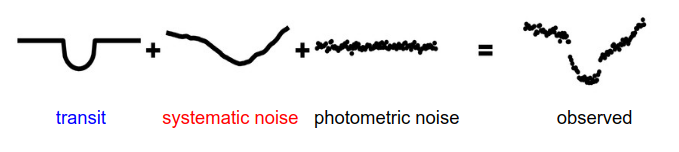
\includegraphics[width=15cm]{figures/noise.png}
\caption{General components of a transit light curve including noise.}
\label{fig:noise_sources}
\end{figure}
%What we would like to do is to model all of them together and at the same time (i.e simultaneous) to get the best fit parameters; not model them separately by removing systematic first and then fitting for transit parameters (or vice-versa).
Because the difference in the expected transit depths at a given passband can be smaller relative to the amplitude of the systematic noise, imperfect systematic correction can easily cause biases in the transit parameters. Hence, systematics should be accounted for correctly to ensure unbiased results.%high photometric accuracy.

As in \cite{Fukui2016a} (see also \cite{Luger2017}), we adapted the usual parameterization of $F_{out}$ as a linear combination of  constant coefficients (or weights), $w$, and observables, $X$,
\begin{equation}
F_{out}= \Big(w_0+\sum w_iX_i \Big) \times F_{in}
%F_{out}=k_0 \times 10^{=0.4 \Delta m_cor}= \sum k_iX_i
\end{equation}
where $X$ contains auxiliary information obtained during the observation such as  target's FWHM, change in stellar position on the detector, airmass, etc. 
%Using Maximum Likelihood Estimation (MLE) to compute/optimize $w$ is not recommended (and will most likely fail) because we don't have good guesses for the initial values of the constant coefficients. Remember in our transit modeling, we have good guesses for limb-darkening coefficients, transit center, etc.

% $w$ is a nuisance parameter\footnote{A nuisance parameter is one that is required in order to model the process that generates the data, but is otherwise of little interest.}
Computing the coefficients $w_i$ is simply doing multiple regression:
$$
y_i=10^{-0.4S}
$$
where 
\begin{equation}
S=w_0+\sum_{i=0}w_iX_i,
\end{equation}
given two or more variables in $X$. In vector form, $y= X \cdot w$ where $w$ can be solved with linear algebra,
\begin{align}
X^T \cdot y& = X^T \cdot X \cdot w \\
w&=(X^T \cdot X)^{-1} \cdot X^T \cdot y 
\end{align}
Here $y$ is the function we want to model (e.g. OOT flux normalized by the transit model) and $X$ can be composed of any auxiliary observables that can reasonably explain the variability, including airmass, centroid position of target in the detector, etc. Since our raw light curves show apparent trend in OOT phase, we included the baseline (i.e. $w_0+w_1t$) as default in the systematic model of each data set. 

There is no rule on how to determine the best or correct set of auxiliary observable to put in $X$. It is reasonable however to use those vectors that are correlated with the function that we want to model. Thus, we first consider observables that are correlated with the OOT phase. A sample pairplot for HAT-P-44b observables is shown in Fig.~\ref{fig:pairplot} which visualizes the correlation among variables. 
\begin{figure}
\centering
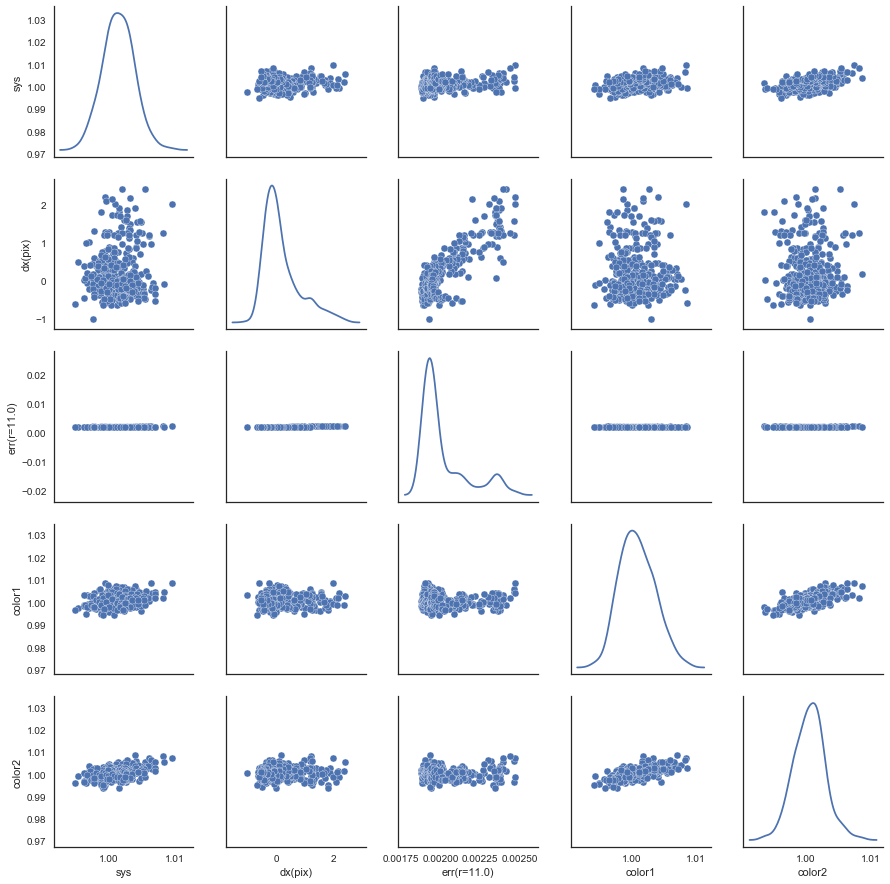
\includegraphics[width=12cm]{figures/best_observables.png}
\caption{An example pair plot of OOT flux and observables showing no apparent correlations (in the off-diagonal) %and density (along diagonal) 
among variables in g-band of HAT-P-44b data set.}
\label{fig:pairplot}
\end{figure}

Intuitively, the more parameters used in the model, the better the fit. 
%When fitting models, it is possible to increase the likelihood by adding parameters, but doing so may result in overfitting. The BIC resolves this problem by introducing a penalty term for the number of parameters in the model.
When selecting a good model however, it should have a balance between goodness of fit and model simplicity. Thus, we use Bayesian Information Criterion (BIC; \cite{Schwarz1978}) to objectively determine which observables to include in the model. BIC is defined as
\begin{equation}
BIC = \chi^2 +d\log N
\end{equation}
where $\chi^2$ is the standard chi-square, $N$ is the number of data points in the light curve and $d$ is the number of dimensions or parameters in the model. Between two competing models, the one with smaller BIC value is preferred. The observables used in each data set and their BIC values are summarized in Table~\ref{tab:bic}. %The adapted observables are shown in bold.
Although a simple 2-parameter baseline model yields lowest BIC value, we adapted a 5-parameter model because it models the variability better especially in the OOT phase. %A separate method for model selection using the Bayesian evidence is discussed in $\S$\ref{sec:model_selection}. The BIC is determined solely from the highest likelihood value, making it easier to calculate than K. Models with lower BIC values are generally favored. Note, however, that the BIC is a less accurate method for distinguishing between models than is K.

\begin{table}
\centering
\caption{BIC values for a representative sample of combinations of observation.}
\label{tab:bic}
\begin{tabular}{lllllllllllll}
model  & \multicolumn{4}{l}{HAT-P-44b}          & \multicolumn{4}{l}{HAT-P-12b}          & \multicolumn{4}{l}{WASP-21b}           \\ \hline
       & BIC & rms & $\beta$ & BIC & rms & $\beta$ & rms$\times\beta$ & BIC & rms & $\beta$ \\
g-band & \multicolumn{12}{l}{}                                                                                                    \\
$k_z$  & 1262.88    & 0.0018    & 1.1515       &   0.002   & 3766    & 0.0019    & 2.5096        &  2825   & 0.0008     & 3.3068                   \\ \hline
r-band & \multicolumn{12}{l}{}                                                                                                    \\
$k_z$  & 2365.70    & 0.0017    & 1.3033       &  0.002    & 6260    & 0.0019    & 2.2240        & 9345    & 0.0011    &  2.6869                   \\ \hline
z-band & \multicolumn{12}{l}{}                                                                                                    \\
       &     &     &         &                 &     &     &         &                  &     &     &         &    \\
$k_z$  & 1211.68    & 0.0020    & 1.3345       &   0.002   & 3010    & 0.0019  &  1.8684       & 4030    &  0.0011   & 2.9127                     \\ \hline
\end{tabular}
\end{table}
                              
\begin{comment}
Fukui et al. (2016) introduced a parameterization of baseline systematics which takes account of the second-order extinction effect. The applied function is:
$$
m_t(t) = M_{tr} + w_0 + w_tt + w_cm_c(t) + \sum w_iX_i
$$
where $m_t$ and $m_c$ are the apparent magnitudes of the target star and comparison stars, respectively, $M_{tr}$ is a transit model in magnitude scale, $t$ is time, $X_i$ is auxiliary observables such as stellar displacements on the detectors, sky backgrounds, and FWHM of the stellar PSFs, and $w_0, w_t, w_c,$ and $w_i$ are coefficients to be fitted.
\end{comment}

\subsection{Optimization\label{sec:optimization}}
We search for the optimum values of transit+systematic model parameters using the Maximum Likelihood Estimation (MLE) approach. This step entails maximizing a likelihood function in Eq.~\ref{eq:likelihood} with $\chi^2$ equal to 
\begin{equation}
\chi^2=\frac{(F_{rel}/F_{out}-F_{in})^2}{\sigma^2}
\end{equation}
where $\sigma$ is the %(inflated) 
photometric uncertainty. 
%From a family of MLE, we used the simplex algorithm \cite{NelderMead1965} implemented in \verb'scipy' library.
%Nelder, J A, and R Mead. 1965. A Simplex Method for Function Minimization. The Computer Journal 7: 308-13
Non-linear optimization is important because the solution for simultaneous transit and systematic models cannot be solved analytically. Finding the optimum values is also important for later analysis involving MCMC (\S \ref{sec:MCMC}). MCMC should be initialized with reasonable starting positions for each parameter in the model, otherwise it will take too long for the solution to converge. Thus, we tried different initial values in case there are different reported values in literature. After several trials, we adopted the optimized values used for later analysis. The result of optimization is illustrated Fig~\ref{fig:hatp44_opt}--\ref{fig:wasp21_opt}. 

\begin{figure}
\centering
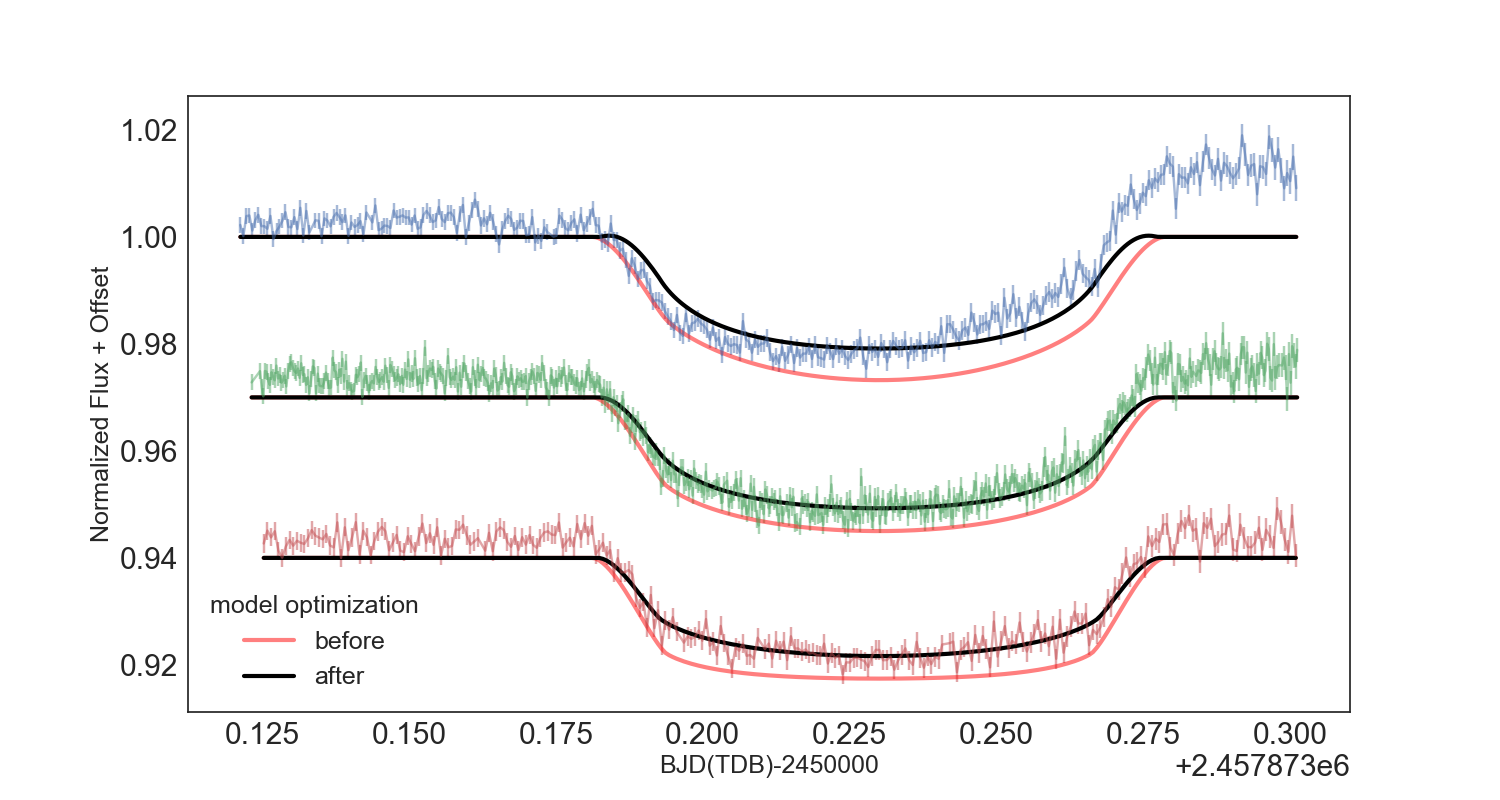
\includegraphics[width=12cm]{hatp44/optimized_transit_model.png}
\caption{Comparison of transit model before (red solid line) and after (black) optimization. As usual, the blue, green, and red light data points with error bars correspond to g-,r-, and z-bands, respectively. The light curves as displaced vertically for clarity.}
\label{fig:hatp44_opt}
\end{figure}

\begin{figure}
\centering
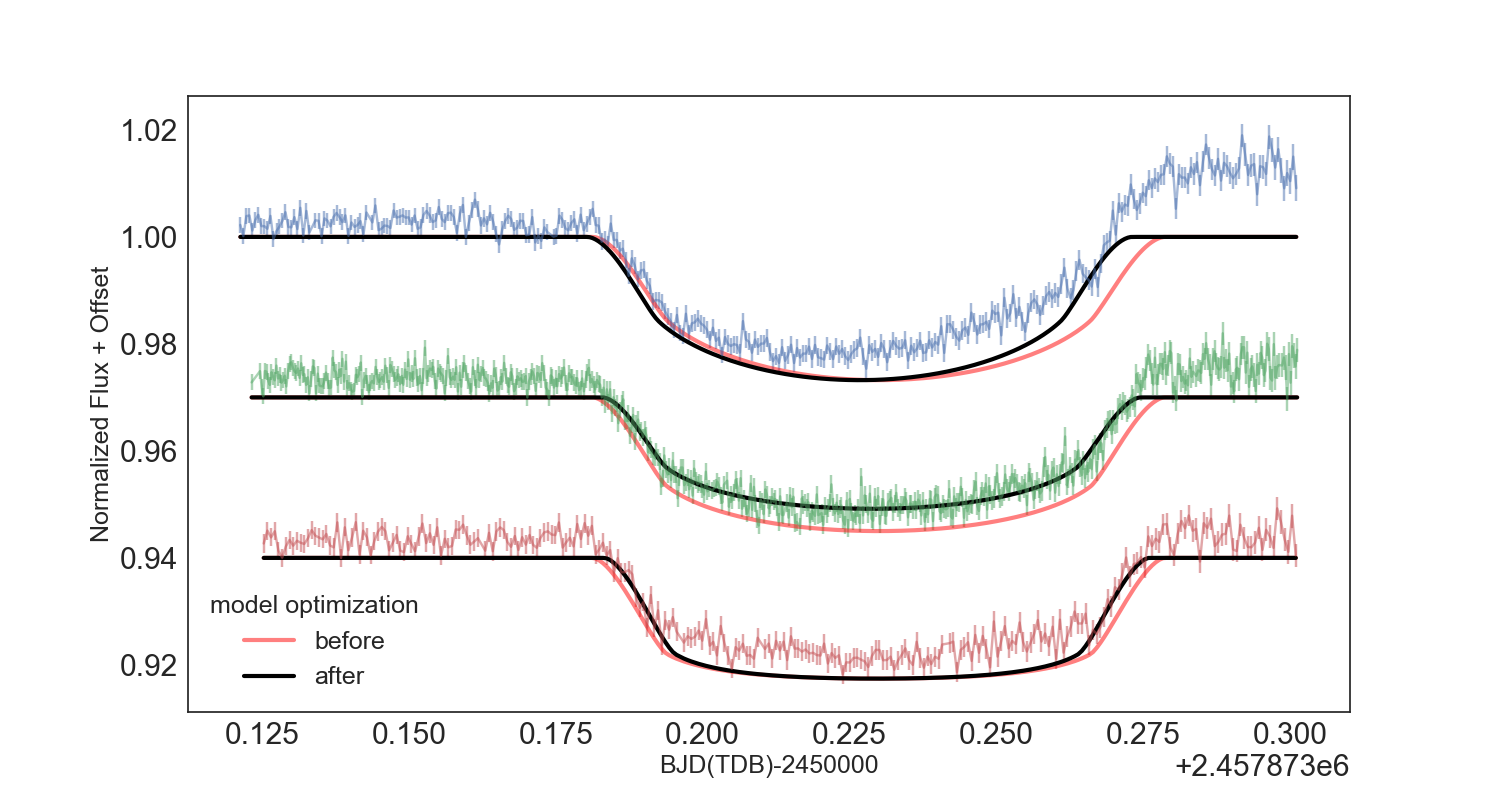
\includegraphics[width=12cm]{hatp12/optimized_transit_model.png}
\caption{Same as Fig.~\ref{fig:hatp44_opt} but for HAT-P-12b.}
\label{fig:hatp12_opt}
\end{figure}

\begin{figure}
\centering
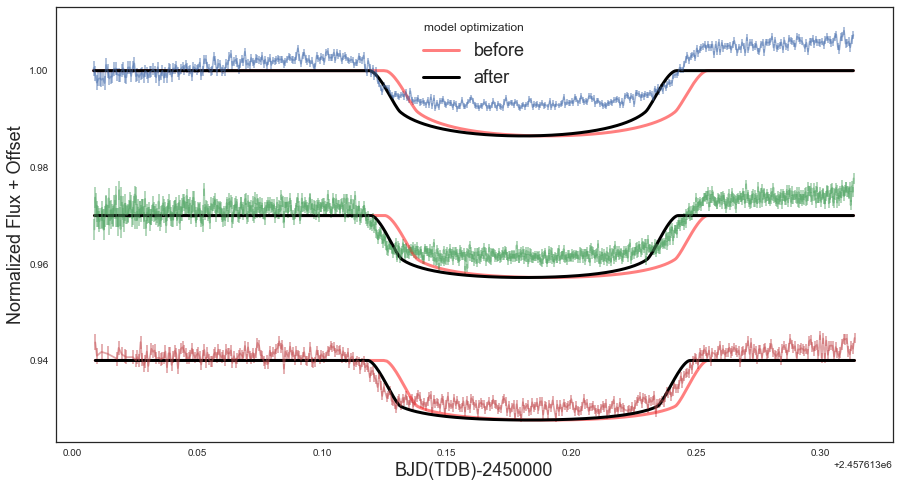
\includegraphics[width=12cm]{wasp21/optimized_transit_model.png}
\caption{Same as Fig.~\ref{fig:hatp44_opt} but for WASP-21b}
\label{fig:wasp21_opt}
\end{figure}

%reduced chi-square
After optimization, we re-scale the photometric errors to take into account possible over-/under-fitting and red noise in the residual. First, we inflate the original estimate of the photometric uncertainty such that the reduced $\chi^2$ for each light curve becomes unity. Reduced $\chi^2$ is defined as
\begin{equation}
red. \chi^2= \frac{\chi^2}{n-d}
\end{equation}
where $n$ is the number of data points and $d$ is the number of parameters.

%beta: time-correlated noise
Second, we estimate the level of time-correlated noise (a.k.a. red noise: Pont et al. 2006) in each light curve, by calculating the $\beta$ factor at various bins (Winn et al. 2008). 
%The $\beta$ factor is used to take into account the time-correlated noise and to properly compensate for the possible underestimation of derived uncertainties from our analysis . 
Specifically, the beta factor is defined as
\begin{equation} \label{eq:beta}
\sigma_N = \frac{\sigma_1}{\sqrt{N}}\sqrt{\frac{M}{M-1}}
\end{equation}
where $\sigma_n$ is the theoretical standard deviation of the binned residuals, $\sigma_1$ is the standard deviation of the unbinned residuals, $N$ is the number of data points per bin, and $M$ is the number of bins. We then compute the median value of $\beta$ for all values of $N$ corresponding to bin widths between 5-20-minute as illustrated in Fig.~\ref{fig:beta} for the case of HAT-P-44b.
%The light curves show significant time-correlated noise, especially in the r- and z-band. 
If the reduced $\chi^2$ and/or $\beta$ is larger than unity, we re-scale the photometric errors of the data; else we preserve the original estimate of the uncertainty to be conservative. The computed $\chi^2$ and $\beta$ values for various binning cases in each color are summarized in Table~\ref{tab:beta}.
Fig.~\ref{fig:rms} shows a similar diagnosis for red noise which compares the rms of the residual as a function of bin size with the theoretical $\sqrt{n}$ decrease expected for Poisson noise.


\begin{figure}
\centering
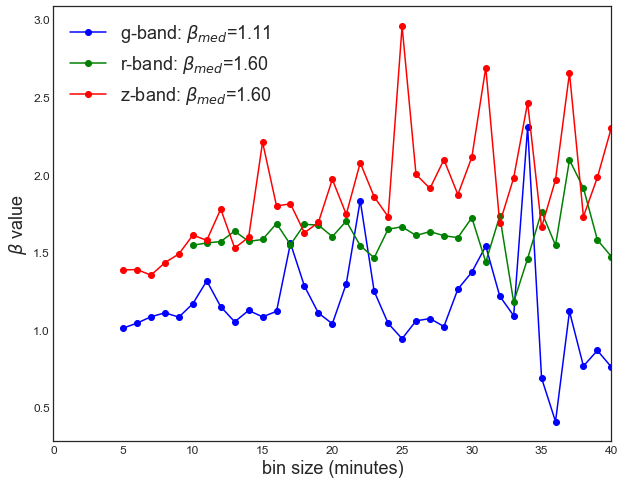
\includegraphics[width=8cm]{figures/beta.png}
\caption{Beta values computed at different binning for HAT-P-44b in each band as a measure of time-correlated (a.k.a. red) noise in the light curve. The median values of betas at all bin-sizes indicated in the upper left are used to inflate the original photometric uncertainties.}
\label{fig:beta}
\end{figure}

\begin{figure}
\centering
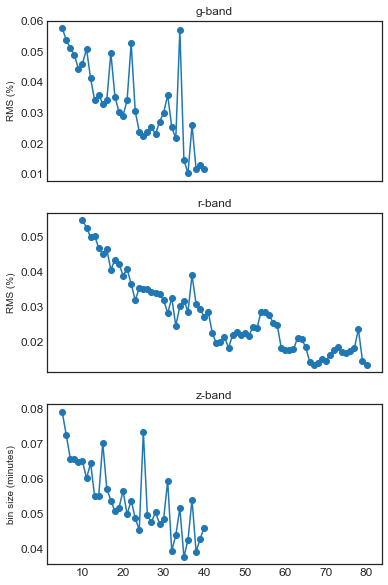
\includegraphics[width=8cm]{figures/binned_rms.png}
\caption{Computed rms error of the residual as function of bin sizes in each color of HAT-P-44b light curve. The monotonic ($\sqrt{n}$) decrease in rms as function of bin size is expected for residual which is purely Poisson noise.}
\label{fig:rms}
\end{figure}

\begin{table}
\centering
\caption{Computed reduced chi-square and beta values used to re-scale the original estimate of photometric uncertainty.}
\label{tab:beta}
\begin{tabular}{llllll}
\multicolumn{2}{l}{}                    & HAT-P-44  & HAT-P-12 & WASP-21 \\ \hline
\multirow{3}{*}{red. $\chi^2$} & g-band: & 1.0963   & 1.4076  & 2.8091\\
                              & r-band: & 1.0971    & 1.6511  & 2.0338\\
                              & z-band: & 1.0487    & 1.2946  & 1.7551\\ \hline
$\beta$                       & g-band: & 1.1515 & 2.5096     & 3.3068 \\
                              & r-band: & 1.3033 & 4.2240     & 4.6869 \\
                              & z-band: & 1.3345 & 1.8684     & 2.9127 \\  \hline
\end{tabular}
\end{table}

\subsection{Markov Chain Monte Carlo \label{sec:MCMC}}
%We derived the maximum posterior probability distributions for the fitted parameters by solving the Bayesian relation and running multiple, very long Monte Carlo Markov Chain (MCMC) simulations of our multivariate model. 
Markov Chain Monte Carlo (MCMC) methods are a class algorithms used to sample from--and thereby provide sampling approximations to--the posterior probability distribution function (PDF) efficiently even in parameter spaces with high number of dimensions. Detailed discussion of MCMC is beyond the scope of this thesis and so only the relevant information is summarized as follows.

The goal of our MCMC simulation is to generate a chain of states, i.e. a chain of sets of model parameters $\theta_i$ that are sampled from the desired posterior PDF $P(\theta|D)$. Using the simple Metropolis-Hastings algorithm for example, such a chain can be computed by specifying an initial set of parameter values, $\theta_0$, and a proposal distribution, $P(\theta$'|$\theta_n)$. At each iteration, a new proposal state $\theta$' is generated and the corresponding model is fit to the data. The new proposal state is then randomly accepted or rejected with a probability that depends on (1) difference between the $\chi^2$-fits of the previous state and the proposal state and (2) difference in the prior probability between previous state and prior state. A proposal state that leads to an improvement in the $\chi^2$-fit and a higher prior probability compared to the previous state is always accepted. The process is repeated long enough until the chains are sufficiently converged. From the posterior PDF, several statistical measures can be computed including the best estimates and Bayesian credible regions. On this note, the prior uncertainties associated with the free parameters are propagated to the final estimate.

Note that MCMC is a necessary step in our transit modeling because the result of the non-linear optimization in \S \ref{sec:optimization} may not necessarily correspond to the global optimum solution. Especially in the case of our modeling which requires exploring large dimensional hyper-surface (>20 free parameters), MCMC is a robust method to obtain such a solution.

\paragraph{MCMC Set-up}
%In the per color set-up, all transit (except period) and systematics model parameters are kept free. 
Instead of modeling light curves individually, we modeled all light curves (g-,r-, and z-bands) simultaneously. The advantage of simultaneous multi-color modeling is leveraging mutual information in each color such as $t_c, b$, and $a_s$ at the expense of having higher total number of parameters. In this set-up, we fitted the three light curves simultaneously by treating $R_p/R_s$ and $q_1, q_2$, and $w$ as independent free parameters for each band while treating $t_c, b$, and $a_s$ as common/ shared (i.e. color-independent) parameter. Except for the period, %passband-dependent
transit parameters and systematics coefficients listed in Table \ref{tab:param_mcmc} are kept free. %As a consistency check, we compare the result of per color modeling and confirm both give consistent results.

\begin{table}
\centering
\caption{Parameter setting matrix for our MCMC run}
\label{tab:param_mcmc}
\begin{tabular}{llllll}
                     & Fixed   & Free   \\ \hline
Shared      & $P$     & $t_c, b, a_s$   \\
Independent &         & $q_{1,i},q_{2,i}, k_i, w_i$ \\
\hline
\end{tabular} \\
\raggedright \textbf{Notes.} The parameters assigned with subscript $i$, are color-dependent. In per color set-up, there are 6 transit parameters and 5 coefficients $w_i$, amounting to 11 free parameters. In the multi-color set-up, $b$, $a_s$, and $t_c$ are shared amounting to 27 free parameters in the MCMC run. 
\end{table}

We use \verb'emcee'\footnote{http://github.com/dfm/emcee}, an affine-invariant ensemble sampler (\cite{Foreman-Mackey2013}) with 256 walkers which ran for 10$^5$ steps starting from the optimized values computed in $\S$\ref{sec:optimization} taken as initial values. 
After discarding the first 10\% steps (i.e. burn-in phase),  
%Gelman-Rubin statistic
we combined the results from all chains and evaluated convergence of each parameter using the Gelman-Rubin statistic $\hat{R}$ (Gelman \& Rubin 1992), and considered the chains to be stabilized %well-mixed 
if $\hat{R} \leq 1.05$ for all parameters. To ensure independent sampling, we constructed the posterior distribution by sampling each chain at intervals spaced by autocorrelation time scale, $\tau$.  %The autocorrelation time is a direct measure of the number of evaluations of the posterior PDF required to produce independent samples of the target density.
%The full set of maximum aposteriori (MAP) values based on the highest log probability should converge to/consistent within one sigma with the individual median values.
% The jump sizes of parameters in each MCMC step are adjusted such that acceptance ratios become ∼23%, which is considered as an optimal acceptance ratio for efficient convergence of MCMC (see e.g., Ford 2005).
We tested for convergence by dividing the chain in two halves and confirmed that they gave consistent results. We also took 10$^3$ independent samples in each chain and plotted the results as shown in Fig.~\ref{fig:hatp44_samples}--\ref{fig:wasp21_samples}.
%The mean values of the parameter traces were then interpreted as the most probable parameters utilizing the 68.3\% highest probability density intervals (HPD) as our error estimate. %For those parameters which require error propagation, such as the impact parameter $b$, we applied the corresponding equation to the MCMC parameter traces; then the HPD of the parameter can be determined from that new distribution.
We checked that maximum posterior probability distributions of wavelength-independent parameters such as scaled semi-major axis, $a/R_s$, impact parameter, $b$, and transit center, $t_c$, 
%stellar density, $\rho_s$ 
are consistent within 1-$\sigma$ in both set-ups. %as shown in Table~\ref{tab:MAP}. 
We define 1$\sigma$ uncertainties by the range of parameters between 15.87\% and 84.13\% of the merged posterior distributions. The results are described in $\S$ \ref{sec:results}. 
%---Analysis and Results
\chapter{Analysis of Results}\label{sec:results}
\section{Marginalized Transit Parameters}

We take the maximum $a\;posteriori$ (MAP) from the MCMC chain as the "best-fit" values summarized in Table~\ref{tab:hatp12_map}--\ref{tab:wasp21_map}. MAP is computed by taking from the chain the set of model parameters with the highest posterior (prior$\times$likelihood) probability. Using the MAP values of each model parameter, we compute the best-fit transit model as well as systematic model which is used to correct or de-trend the raw data. The systematics-corrected light curves and root mean square (rms) error are shown in Fig.~\ref{fig:hatp44_grz_multi}--\ref{fig:wasp21_grz_multi}. %We also report other summary statistics to better describe the shape of the distribution of each parameter of interest in Table~\ref{tab:hatp44_summary}--\ref{tab:wasp21_summary}.
In the following, we compare the results of our transit modeling with published values. %We discuss our result for Rp/Rs separately in $\S$\ref{sec:spectrum}.

%------------------------------------------------------------------------
\paragraph{HAT-P-12b}
It is important to check whether our results agree with published values especially in the case of HAT-P-12b which has been observed extensively. Assuming stellar radius in R$_s$= 0.959 $\pm$ 0.02 R$_{\odot}$ in Table~\ref{tab:params}, the measured mean planet radius is 0.955$^{+0.006}_{-0.010}$ R$_J$ compared to the published 0.96$^{+0.03}_{-0.02}$ R$_J$, a difference of $\sim$0.5\% which is well within the published uncertainty. Propagating the uncertainty in stellar radius however, we see that the uncertainty in R$_p$ cannot be any less than 0.13 R$_J$.

For impact parameter, we get $b$=0.23 $\pm$ 0.14 compared to the published 0.211$^{+0.066}_{-0.078}$, a difference of $\sim$ 9\%. The large uncertainties in $b$ is reflected from the wide posterior in Fig.~\ref{fig:hatp12_tab}. For scaled semi-major axis, a/Rs=11.6197$\pm$0.1809 compared to the published 11.77$\pm$0.21, a difference of $\sim$1.3\% with smaller uncertainty. Therefore, $b$ and a$_s$ agree well with values found by \cite{Hartmann2009}.
Moreover, the mean stellar density, $\rho_s$, can be directly derived from a/Rs and P via the the Eq.~\ref{eq:rho_star} assuming a circular orbit. From our MCMC results, we derive the stellar density to be $\rho_s$ = 2.92$_{-0.16}^{+0.14}$, which is consistent with the average density of 3.00$\pm0.27$ g/cm$^3$ solely determined from published mass and radius.

The full joint posterior distributions of transit center, $t_c$, impact parameter, $b$, and scaled semi-major axis, a$_s$ are shown in Fig~\ref{fig:hatp12_tab}. Summary plots of other transit parameters shown in Fig.~\ref{fig:hatp12_q1q2}.
%The four values in each parameter are largely consistent with each other. To compare them with the results of previous work we also list the values from Southworth (2012) who derived them by analyzing nine published light curves that were obtained with 1–2 m class telescopes, including five with the FLWO 1.2 m telescope (Torres et al. 2010), two with the 2.0 m LT (Simpson et al. 2011), one with the 2.0 m FTN (Simpson et al. 2011), and one with the Asiago 1.82 m telescope (Nascimbeni et al. 2011). The values from the joint fit to all the MuSCAT light curves are consistent with those from Southworth (2012) within the uncertainties.

%In addition the uncertainties from MuSCAT are smaller than those from Southworth (2012), meaning that MuSCAT provides the highest-quality transit data of this planet from only a single transit observation. The light curves of MuSCAT corrected by the best-fit OOT models and the residual light curves from the best-fit transit models are shown in Figure 2. The root mean square (rms) values of the unbinned (five minutes binned) residual light curves are 0.10\% (0.028\%), 0.091\% (0.022\%), and 0.068\% (0.024\%) for the g, r, and z bands, respectively. In Figure 3 we show the rms values of binned residual light curves as a function of binning size. The black lines indicate the observed data while the orange dashed, light blue dashed–dotted, magenta dotted, green three-dotted–dashed, and gray solid lines represent expected values from scintillation noise, photon noise from the target star, photon noise from the comparison stars, sky background noise, and the total of them, respectively.
 
%------------------------------------------------------------------------
\begin{table}
\centering
\caption{System parameters and 1$\sigma$ error limits derived from the MCMC analysis of HAT-P-12b light curve. The reported 1-$\sigma$ uncertainties correspond to 16\% and 84\% percentiles of its posterior distribution.}
\begin{tabular}{ccccccc}
\multicolumn{2}{l}{}                           & This work & Hartmann+09 \\ \hline
\multirow{3}{*}{$R_p/R_s$}& g-band:      & 0.14196$_{-0.00404}^{+0.00058}$   & - \\
                          & r-band:      & 0.14024$_{-0.00150}^{+0.00092}$   & - \\
                          & z-band:      & 0.14025$_{-0.00481}^{+0.00114}$   & - \\ \hline
R$_p$ [R$_J$]             & & 0.955$^{+0.006}_{-0.010}$ & 0.96$^{+0.03}_{-0.02}$\\
$q_1, q_2$                & g-band:      & 0.6174, 0.5196   & -     \\
                          & r-band:      & 0.5570, 0.4214   & -     \\
                          & z-band:      & 0.4070,  0.1716  & -     \\ \hline
\multicolumn{2}{l}{Transit epoch, $T_0$ (HJD)} & 2457873.2292	  &      \\
\multicolumn{2}{l}{a/Rs}                     & 11.6197$\pm$0.1809 & 11.77$\pm$0.21 \\
\multicolumn{2}{l}{Impact parameter, $b$}    & 0.23 $\pm$ 0.14  & 0.211$^{+0.066}_{-0.078}$  \\
\multicolumn{2}{l}{inclination (deg)}        & 89.3             & 89.0$\pm$0.4  \\  
\multicolumn{2}{l}{star density $\rho_s$ (g/cm$^3$)}        & 2.92$_{-0.16}^{+0.14}$  &  --  \\  
\hline  
\label{tab:hatp12_map}
\end{tabular}
\end{table}

\begin{table}
\centering
\caption{Same as Table~\ref{tab:hatp12_map} but for HAT-P-44. Results are compared with values in Hartmann et al. 2014.}
\begin{tabular}{ccccccc}
\multicolumn{2}{l}{}                     & This work                    & Hartmann+14 \\ \hline
\multirow{3}{*}{$R_p/R_s$}& g-band:      & 0.13182$_{-0.00102}^{+0.00133}$        &  \\
                          & r-band:      & 0.13294$_{-0.00157}^{+0.00018}$        &  \\
                          & z-band:      & 0.13109$_{-0.00179}^{+0.00092}$        &  \\ \hline
R$_p$ [R$_J$]             & & 1.228$\pm$ 0.0147 & 1.242$\pm$ 0.106 \\
$q_1, q_2$                & g-band:      & 0.5814, 0.4540 &  \\
                          & r-band:      & 0.5100, 0.3427 &  \\
                          & z-band:      & 0.3375, 0.2564 &  \\ \hline
\multicolumn{2}{l}{Transit epoch, $T_0$ (HJD)} & 2457800.2199   &  \\
\multicolumn{2}{l}{a/Rs}                   & 12.0440$\pm$0.0094 &  11.49$^{+0.46}_{-0.85}$ \\
\multicolumn{2}{l}{Impact parameter, $b$}  & 0.16$\pm$0.13  &  0.172$\pm$0.079 \\
\multicolumn{2}{l}{inclination (deg)}      & 89.6           &  89.10 \\ 
\multicolumn{2}{l}{star density $\rho_s$ (g/cm$^3$)}        & 1.84$_{-0.05}^{+0.03}$  &  --  \\  
\hline  
\label{tab:hatp44_map}
\end{tabular}
\end{table}

\begin{table}
\centering
\caption{Same as Table~\ref{tab:hatp12_map} but for WASP-21b. Results are compared with values in Bouchy et al. 2010.}
\label{tab:wasp21_map}
\begin{tabular}{ccccccc}
\multicolumn{2}{l}{}                     & This work            & Bouchy+10 & \\ \hline
\multirow{3}{*}{$R_p/R_s$}& g-band:      & 0.09670$^{-0.00040}_{+0.00155}$ & -  & \\
                          & r-band:      & 0.09889$^{-0.00039}_{+0.00059}$ & -  & \\
                          & z-band:      & 0.09998$^{-0.00043}_{+0.00092}$ & -  & \\ \hline
R$_p$ [R$_J$]             & & 1.097 $\pm$ 0.0044 & 1.07$\pm$ 0.06 \\
$q_1, q_2$                & g-band:      & 0.5060, 0.3329 & - & \\
                          & r-band:      & 0.3807, 0.2420 & - & \\
                          & z-band:      & 0.2484, 0.2780 & - & \\ \hline
\multicolumn{2}{l}{Transit epoch, $T_0$ (HJD)} & 2457613.1832 & - & \\
\multicolumn{2}{l}{a/Rs}                     & 10.09$\pm$0.12 & 9.62$\pm$0.17 \\
\multicolumn{2}{l}{Impact parameter, $b$}    & 0.3673 $\pm$ 0.0089 & 0.23 &   \\
\multicolumn{2}{l}{inclination (deg)}        & 89.88       & 88.75 & \\  
\multicolumn{2}{l}{star density $\rho_s$ (g/cm$^3$)}        & 1.023$_{-0.018}^{+0.032}$ & 0.855$\pm$0.068  \\  
\hline  
\end{tabular}
\end{table}

\begin{figure}
\centering
	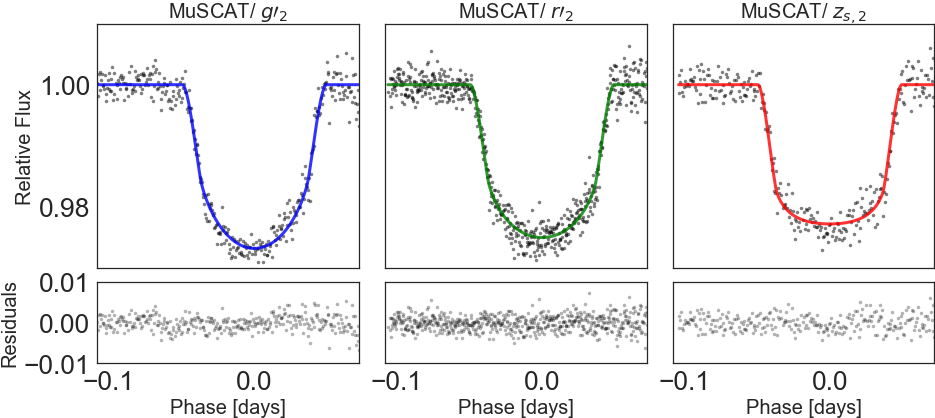
\includegraphics[width=1\columnwidth]{hatp12/grz_with_rms.png}
    \caption{Systematics-corrected transit light curves for HAT-P-44b (black dots) and best-fit transit models. %The binned flux data for $g'$, $r'$, and $z_s$-bands are shown by the blue, green, and red squares, respectively. 
    The blue, green, and red lines indicate the best-fit transit models for $g'$, $r'$, and $z_s$-bands. The lower panels show the residuals which have rms of 0.17\%,0.17\%,and 0.19\% for $g'$, $r'$, and $z_s$-bands respectively.}
\label{fig:hatp12_grz_multi}
\end{figure}

\begin{figure}
	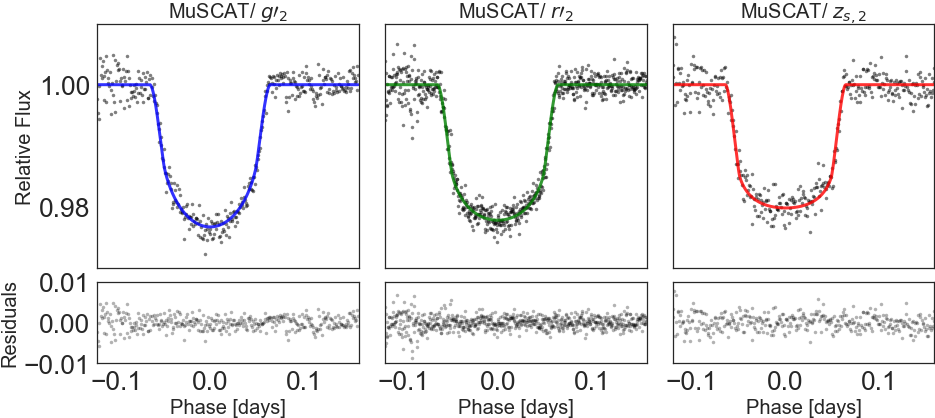
\includegraphics[width=1\columnwidth]{hatp44/grz_with_rms.png}
    \caption{Same as Fig.~\ref{fig:hatp12_grz_multi} but for HAT-P-12b. The lower panels show the residuals which have rms of 0.08\%,0.11\%,and 0.11\% for $g'$, $r'$, and $z_s$-bands respectively. %How about for n-minute bins?
    }\label{fig:hatp44_grz_multi}
\end{figure}

\begin{figure}
	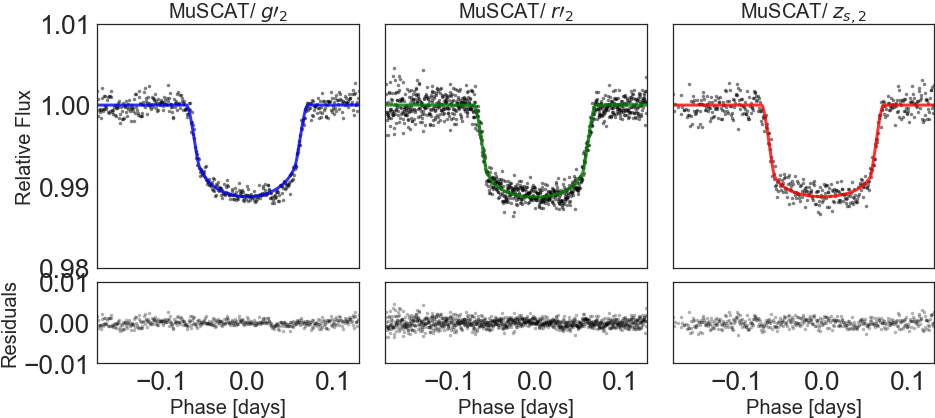
\includegraphics[width=1\columnwidth]{wasp21/grz_with_rms.png}
    \caption{Same as Fig.~\ref{fig:hatp44_grz_multi} but for WASP-21b. The lower panels show the residuals which have rms of 0.20\%,0.20\%,and 0.22\% for $g'$, $r'$, and $z_s$-bands respectively. %How about for n-minute bins?
    }\label{fig:wasp21_grz_multi}
\end{figure}

%Our results are in general agreement with those obtained by Hartman et al. (2009), Lee et al. (2012), and Sada et al. (2012).
%However, the recent analysis of a near-IR transmission spectrum from Hubble Space Telescope data by Line et al. (2013) yields a planet-to-star radius ratio that is ∼2.5\% smaller than the others

\paragraph{HAT-P-44b}
%See O-C diagram here
%http://var2.astro.cz/ETD/etd.php?STARNAME=HAT-P-44&PLANET=b
%HAT-P-44b since only single observation has been conducted towards this system. 
Assuming stellar radius in R$_s$= 0.95 $\pm$ 0.08 R$_{\odot}$ in Table~\ref{tab:params}, the measured mean planet radius is 1.228$\pm$ 0.015 R$_J$ compared to the published 1.242$\pm$ 0.106 R$_J$, a difference of $\sim$1.1\% which is well within the published uncertainty. Propagating the uncertainty in stellar radius however, we see that the uncertainty in R$_p$ cannot be any less than 0.7 R$_J$.

For impact parameter, we get $b$=0.16 $\pm$ 0.13 compared to the published 0.172$\pm$0.079, a difference of $\sim$ 9.5\%. Like HAT-P-12b, the large uncertainty in $b$ is reflected from the wide posterior in Fig.~\ref{fig:hatp44_tab}. For scaled semi-major axis, a/Rs=12.0440$\pm$0.0094 compared to the published 11.49$^{+0.46}_{-0.85}$, a difference of $\sim$4.8\% with smaller uncertainty. Therefore, $b$ and a$_s$ agree well with values found by \cite{Hartmann2014}. Moreover, the mean stellar density, $\rho_s$, is 1.84$_{-0.05}^{+0.03}$, which is consistent with the average density of 1.55$\pm$0.36 g/cm$^3$ solely determined from published mass and radius.

The full joint posterior distributions of transit center, $t_c$, impact parameter, $b$, and scaled semi-major axis, a$_s$ are shown in Fig~\ref{fig:hatp44_tab}. $t_c$, $b$, and a$_s$ agree well with values found by \cite{Hartmann2014}. Summary plots of other transit parameters shown in Fig.~\ref{fig:hatp44_q1q2}.

\begin{figure}
\centering
	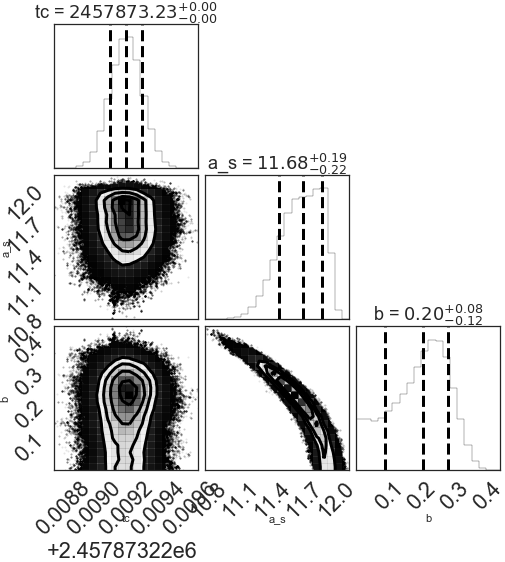
\includegraphics[width=8cm]{hatp12/joint_tc_a_b.png}
    \caption{Joint posterior probability distributions for transit center $t_c$ (columns 1), scaled semi-major axis, a$_s$ (columns 2), and impact parameter, $b$ (columns 3), from which the maximum $a \; posteriori$ (aka "best-fit" values) are computed. The plots on the diagonal are the marginalized posterior distribution where the vertical lines correspond to the adapted MAP and 1-$\sigma$ uncertainties.
    }
\label{fig:hatp12_tab}
\end{figure}

\begin{figure}
\centering
	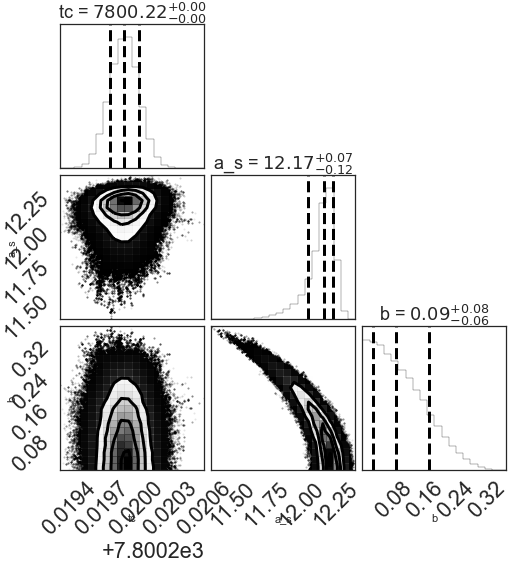
\includegraphics[width=8cm]{hatp44/joint_tc_a_b.png}
	\caption{Same as in Fig.~\ref{fig:hatp12_tab} but for HAT-P-44b.}
\label{fig:hatp44_tab}
\end{figure}

\begin{figure}
\centering
	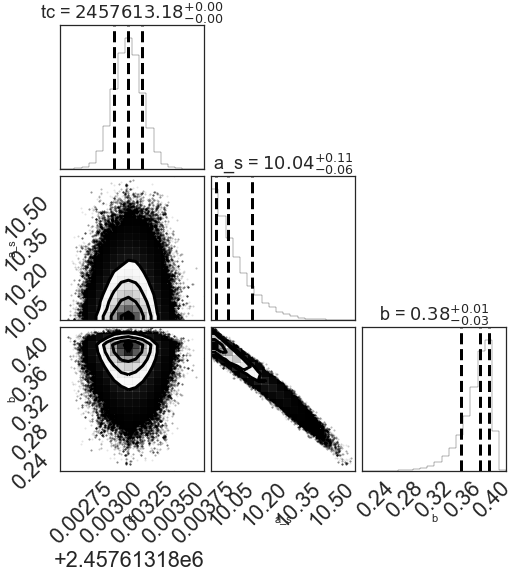
\includegraphics[width=8cm]{wasp21/joint_tc_a_b.png}
    \caption{Same as in Fig.~\ref{fig:hatp12_tab} but for WASP-21b.}
\label{fig:wasp21_tab}
\end{figure}

%------------------------------------------------------------------------
\paragraph{WASP-21b}
%See O-C diagram here
%http://var2.astro.cz/ETD/etd.php?STARNAME=WASP-21&PLANET=b

Assuming stellar radius in R$_s$= 1.136 $\pm$ 0.051 R$_{\odot}$ in Table~\ref{tab:params}, the measured mean planet radius is 1.097 $\pm$ 0.0044 R$_J$ compared to the published 1.07$\pm$ 0.06 R$_J$,
a difference of $\sim$2.5\%. %which is well within the published uncertainty. 
Therefore, we rule out the larger radius R$_p=$1.263$\pm$0.090 found by \cite{Southworth2012} including the fact that it reported larger uncertainties in R$_s$.
In any case, propagating the uncertainty in stellar radius however, we see that the uncertainty in R$_p$ cannot be any less than 0.55 R$_J$.

For impact parameter, we get $b$=0.3673 $\pm$ 0.0089 compared to the published 0.23$\pm$0.015, a difference of $\sim$ 60\% but still within the published uncertainty. Unlike our results for HAT-P-12b and HAT-P-44b, WASP-21b has smaller uncertainties in $b$ as reflected from the narrow posterior in Fig.~\ref{fig:wasp21_tab}. For scaled semi-major axis, a/Rs=10.10$\pm$0.12 compared to the published 9.62$\pm$0.17, a difference of $\sim$4.9\% with smaller uncertainty. Therefore, $b$ and a$_s$ agree well with values found by \cite{Bouchy2010}. Moreover, the mean stellar density, $\rho_s$, is 1.023$_{-0.018}^{+0.032}$, which is consistent with the average density of 0.855$\pm$0.068 g/cm$^3$.

The full joint posterior distributions of transit center, $t_c$, impact parameter, $b$, and scaled semi-major axis, a$_s$ are shown in Fig~\ref{fig:wasp21_tab}. Summary plots of other transit parameters shown in Fig.~\ref{fig:wasp21_q1q2}.


\begin{comment}
#measured Rp/Rs
g-band:	0.13182	$^{-0.00102}_{+0.00133}$
r-band:	0.13294	$^{-0.00157}_{+0.00018}$
z-band:	0.13109	$^{-0.00179}_{+0.00092}$

#measured Rp/Rs
g-band:	0.14196	$^{-0.00404}_{+0.00058}$
r-band:	0.14024	$^{-0.00150}_{+0.00092}$
z-band:	0.14025	$^{-0.00481}_{+0.00114}$

#measured Rp/Rs
g-band:	0.09670	$^{-0.00040}_{+0.00155}$
r-band:	0.09889	$^{-0.00039}_{+0.00059}$
z-band:	0.09998	$^{-0.00043}_{+0.00092}$
\end{comment}


%The uncertainty of individual parameters introduced by non-Gaussian correlations with other parameters is accounted for in a straightforward way by marginalizing the joint posterior over all remaining parameters (\cite{Benneke2012}). 

%in the JWST era
% ephemeris 
%lower uncertainties in:
% orbital period of 4.3012 d 
% mass of 0.35 M$_J$ and 
% radius of 1.24 R$_J$

%------------------------------------------------------------------------
\section{Improved Transit Ephemeris}
% Transit timing became one of the standard techniques in the analysis of transit observations. Commonly the mid-time of each transit observation is plotted into an observed minus calculated (O-C) diagram (Ford \& Holman 2007), where the difference between the observed transit mid-time and the mid-time obtained using the initial ephemeris is shown versus the observing epoch. In such a diagram, a non-zero slope indicate a varying orbital period, while e.g. periodic deviations from a linear trend indicate perturbing forces. %Transit intervals indicating deviations from a strictly Keplerian motion and thus yet hidden planets in the observed system.

The addition of even a single follow-up transit measurement can improve the ephemeris of the planet especially in the case of HAT-P-44b which was observed only a few epochs as reported in the discovery paper. For each planet we analyze in this work, we compute updated ephemerides using the mid-transit times from our work reported in Table~\ref{tab:hatp12_map}--\ref{tab:wasp21_map} and $T_0$ from the discovery paper: % of the previous observations:
\begin{equation}
T_c(BJD_{TDB})=T_0+E \times P
\end{equation}
where $E$ is the epoch and $P$ is the orbital period. 

\paragraph{HAT-P-44b}
To check if our result is consistent with other observation, we enlarged the sample by considering mid-transit times available in the literature or on websites such as the Exoplanet Transit Database (ETD)\footnote{http://var2.astro.cz/ETD/} %TRansiting ExoplanetS and CAndidates (TRESCA) archive, 
which essentially contain light curves obtained by amateur astronomers. We selected only the light curves with a data quality index higher than 3. %(see Table~\ref{tab:hatp44_ephem}). 
By fitting these data with a linear function, we derive the improved transit ephemeris as
\begin{equation}
T_c(\rm{BJD_{TDB}})= 2457800.21961500+4.30119154 \times E
\end{equation}
where $E$ is the relative transit epoch and the number in parentheses on the right represents the last two digits of 1$\sigma$ uncertainty. %The residuals from this ephemeris, $\Delta T_c$, are appended to Table~\ref{tab:hatp44_ephem} and shown in Figure~\ref{fig:hatp44_ephem}.
 
%bivariate correlated errors and intrinsic scatter 

\begin{comment}
\begin{table}
\centering
\label{tab:hatp44_ephem}
\caption{A comparison between the results obtained in our analysis and the literature data for the measured Transit Timing ($Tc$), Timing Residual from the Linear Ephemeris ($T_c$), and Impact Parameter ($b$) for each transit of HAT-P-44b}
\begin{tabular}{lllll}
Transit epoch & Telescope & $T_c$ (BJD$_{TDB}$-2450000) & $\Delta T_c$ (days) & $b$ \\
\hline
0 & OAO188 & 7800.219893$^{0.00013}_{-0.00013}$ &  & \\
\hline
\end{tabular}
\end{table}
\end{comment}

\paragraph{HAT-P-12b}
%https://exoplanetarchive.ipac.caltech.edu/cgi-bin/DisplayOverview/nph-DisplayOverview?objname=HAT-P-12+b&type=CONFIRMED_PLANET
For HAT-P-12b, we derive the improved transit ephemeris as
\begin{equation}
T_c(\rm{BJD_{TDB}})= 2454419.19570000+3.21604609 \times E
\end{equation}
where $E$ is the relative transit epoch and the number in parentheses on the right represents the last two digits of 1$\sigma$ uncertainty.
The residuals from this ephemeris %, $\Delta T_c$, are appended to Table~\ref{tab:hatp12_ephem} and 
is shown in Figure~\ref{fig:hatp12_ephem}.

\begin{comment}
\begin{table}
\centering
\label{tab:hatp12_ephem}
\caption{Same as Table~\ref{tab:hatp44_ephem} but for HAT-P-12b.}
\begin{tabular}{lllll}
Transit epoch & Telescope & $T_c$ (BJD$_{TDB}$-2450000) & $\Delta T_c$ (days) & $b$ \\
\hline
X & FLWO 1.2m & 4419.19556$\pm$0.00020 &  & - \\ %Sada&Ramon-Fox+2016
X & UdMO 0.36m &4419.19584$\pm$0.00009 & & 0.211$^{+0.066}_{-0.078}$ \\ %Hartmann+2009
0 & OAO 1.88m & 7873.2292$\pm$0.0001 &  & 0.211$\pm$0.1402 \\ 
\hline
\end{tabular} 
\end{table}
\end{comment}

\begin{comment}
%2454419.19584±0.00009 (Sada & Ramón-Fox 2016)
%2454419.19556±0.00020 (Hartmann 2009)
%2457613.1832 ± (this study)
%See O-C diagram here
%http://var2.astro.cz/ETD/etd.php?STARNAME=HAT-P-12&PLANET=b
\end{comment}

\paragraph{WASP-21b}
%https://exoplanetarchive.ipac.caltech.edu/cgi-bin/DisplayOverview/nph-DisplayOverview?objname=WASP-21+b&type=CONFIRMED_PLANET
For WASP-21b, we derive the improved transit ephemeris as
\begin{equation}
T_c(\rm{BJD_{TDB}})= 2454743.03822454+4.32251406 \times E
%2454743.04632158+4.32250054xE (with other data)
\end{equation}
%where $E$ is the relative transit epoch and the number in parentheses on the right represents the last two digits of 1$\sigma$ uncertainty.
%Ciceri+2013: T0(BJD_TDB) = 2 454 743.04054 (71)+ 
%                 4.322 5186(30) E
%Seelinger+2015:  4.322 51(22)
%Bouchy+2010:     4.322 4(24)  # −0.000 019
%Barros+2011:     4.322 50(31)
%Southworth+2012: 4.322 50(31)

The residuals from this ephemeris%, $\Delta T_c$, are appended to Table~\ref{tab:wasp21_ephem} and
is shown in Figure~\ref{fig:wasp21_ephem}.
%Selinger+2015: A new ephemeris is determined for the system, i.e. T0= 245 5084.519 74 ± 0.000 20 (HJD) and P= 4.322 5060 ± 0.000 0031 d. 
%In addition, the results of the analysis of two transit events of Ciceri et al. (2013) and one transit observation of Southworth (2012) are also taken into account. Concerning the O-C diagram, we found that a period change of (2.63 ± 0.17) s removes the linear trend which is present in the data fitted with the initial ephemeris. 

\begin{comment}
Seelinger+2015
However, regarding inclination and reverse fractional stellar radius
we do see a significant difference between our results and the
initial values published by Bouchy et al. (2010). This was also found
by other authors before. As discussed in Barros et al. (2011), this
result is a consequence of the assumption of Bouchy et al. (2010)
that the planet host star is a main-sequence star, while Barros et al.
(2011) found that the star starts evolving off the main sequence and
thus its radius increases. This in turn leads to corrections of the
stellar and hence planetary properties.

\begin{table}
\centering
\label{tab:wasp21_ephem}
\caption{Same as Table~\ref{tab:hatp44_ephem} but for WASP-21b.}
\begin{tabular}{lllll}
Transit epoch & Telescope & $T_c$ (BJD$_{TDB}$-2450000) & $\Delta T_c$ (days) & $b$ \\
\hline
X & YETI      & 4743.04217$\pm$0.00065 & & - \\ %Seelinger+2011
X & FLWO 1.2m & 4743.0419$^{+0.0019}_{-0.0022}$&  & 0.23$^{+0.12}_{-0.15}$ \\ %Bouchy+2010
0 & OAO 1.88m & 7873.2292$\pm$0.001 & & 0.2299$\pm$0.1404 \\
\hline
\end{tabular}
\end{table}
\end{comment}

\section{Transit Timing Variation and Transit Duration Variation}
The central times of the transits are also useful to check for the presence of additional bodies. If another planetary object is a member of the system, it should gravitationally interact with the known planet, causing a periodical variation in $T_0$. Other
phenomena can cause timing variations, for example starspots. %(\cite{Barros2013})
We plot the residuals of the linear fits to the times of minimum light below. In both cases we do not find any clear evidence of periodic variations in the transit timings.

\begin{figure}
\centering
	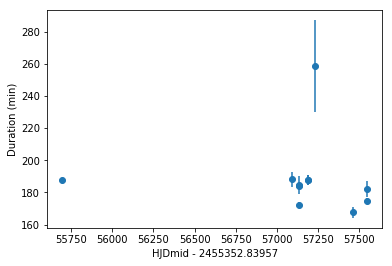
\includegraphics[width=7cm]{hatp44/tdv.png}
    \caption{Updated O-C diagram of HAT-P-44b.}
\label{fig:hatp44_tdv}
\end{figure}

\begin{figure}
\centering
	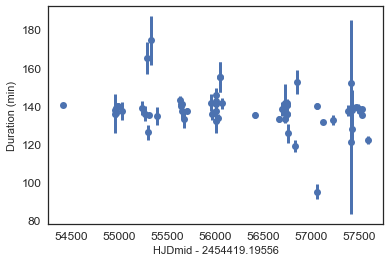
\includegraphics[width=7cm]{hatp12/tdv.png}
    %\caption{Transit duration variation of HAT-P-12b.}
    \caption{Updated O-C diagram of HAT-P-12b. %The transit midpoint at various epochs can be fit with a linear ephemeris.
    }
\label{fig:hatp12_tdv}
\end{figure}
\begin{figure}
\centering
	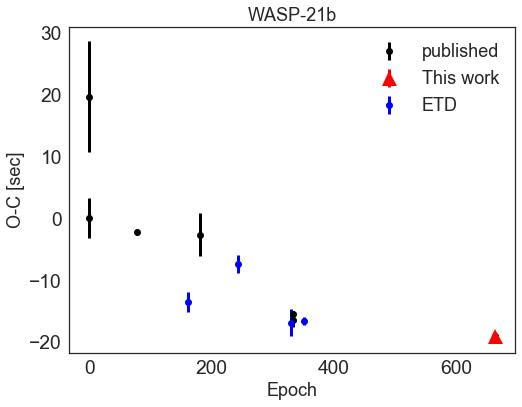
\includegraphics[width=7cm]{wasp21/wasp21_tdv.png}
    \caption{Updated O-C diagram of WASP-21b. %The transit midpoint at various epochs can be fit with a linear ephemeris.
    }
\label{fig:hatp12_oc}
\end{figure}

\begin{comment}
\begin{table}
\centering
\caption{}
\begin{tabular}{lllllll}
& $T_c$ - 2450000 & a/Rs & Rp/Rs & i \\
\hline
Bouchy et al. (2010) &4743.0426 ± 0.0022 & 6.05$^{+0.03}_{−0.04}$ &0.1040$^{+0.0017}_{−0.0018}$ &88.75 $^{+0.70}_{−0.84}$ \\
Barros et al. (2011a) &5084.52048 ± 0.00020 & 9.68 $^{+0.30}_{−0.19}$ &0.1071$^{+0.0009}_{−0.0008}$ & 87.34 ± 0.29 \\
Southworth (2012) &5084.52040 ± 0.00016 &9.35 ± 0.34 &0.1095 ± 0.0013 &86.77 ± 0.45 \\
Ciceri et al. (2013) &4743.04054 ± 0.00071 &9.46 ± 0.27 &0.1055 ± 0.0023 & 86.97 ± 0.33 \\
Seelinger et al. (2015) &4743.04217 ± 0.00065 &9.62 ± 0.17 &0.1030 ± 0.0008 &87.12 ± 0.24 \\
This work & 7613.1832 & 10.0979 & 0.1000 ± 0.005 & \\
\hline
\end{tabular}
\end{table}
\end{comment}

\begin{comment}
The residuals from this ephemeris, $\Delta T_c$, are appended to Table 5 and shown in Figure 4. The $\chi^2$ value of the linear fit is 15.5 for five degrees of freedom (DOF), meaning that the linear function nominally has a 2.6 $\sigma$ discrepancy with the observed data. However, discrepancies with similar levels often arise in ground-based T_c observations, possibly due to unknown systematics rather than the true timing variations. Therefore, we do not consider it to be a noticeable TTV signal at this point. We note that the $T_c$ value of the transit observed by Nascimbeni et al. (2011) departs from our new ephemeris by 2.8$\sigma$, causing a systematic shift in their ephemeris (gray dashed line in Figure 4), which has propagated to be $\sim$ 15 minutes at the time of our observation. In any case, the correction of the ephemeris in this work should be useful for future observations.

Next we search for TDVs to check for any evidence of
additional bodies. The transit duration is generally expressed as
the time interval between the first and fourth contacts of a
transit, T 14 , which is a function of a R s , b, and R p R s . We here assume that a R s and R p R s do not vary with time within the
uncertainties and search for the time dependence of b instead of
T 14 . The measured b values of the seven transits and their
uncertainties are listed in Table 5 and shown in Figure 5. A
constant fit to these values gives the mean of b = 0.9015±0.0024 with c 2 = 7.5 for dof = 6, meaning that no significant variation is observed.

To demonstrate the increased observing efficiency afforded by our MuSCAT observations, we compute the propagated timing uncertainty in %in mid-2019
\begin{equation}
\sigma(t_c)=\sqrt{\sigma(t_0)^2+(n\sigma (P))^2}
\end{equation}
where $\sigma (t_c)$ is the propagated timing uncertainty, $\sigma(t_0)$ is the uncertainty in the starting transit center, $n$ is the number of orbits into the future for which to compute the propagated uncertainty, and $\sigma (P)$ is the uncertainty in the orbital period. 
\end{comment}

We note that the transit midpoint at various epochs can be fit with a linear ephemeris for all planets, consistent with previous results.

\section{Transit Depth Variation}\label{sec:spectrum}
%Caveat
%Stellar variability, in the form of star spots and faculae, can affect the measured transit depth of an exoplanet and hence its spectrum and retrieved physical properties (Pont et al. 2008; Silva Valio 2008; Czesla et al. 2009; Wolter et al. 2009; Agol et al. 2010; Berta et al. 2011; Carter et al. 2011; Desert et al. 2011; Sing et al. 2011; Fraine et al. 2014; McCullough et al. 2014; Oshagh et al. 2014; Damasso et al. 2015; Barstow et al. 2015; Zellem et al. 2015; Rackham et al. 2017). As a worst case scenario for very active stars, unocculted spots can cause an underestimation of the planet-to-star radius ratio of up to 4% at near-infrared wavelengths and 10% at visible wavelengths while faculae can cause an overestimation of the planet-to-star radius ratio of up to ∼0.2% at near- infrared wavelengths at ∼3% at visible wavelengths (Oshagh et al. 2014). Unocculted spots can also mimic a Rayleigh scattering slope indicative of haze; for example, the visible and near-IR slope of the exoplanet HD 189733b’s transit absorption spectrum, interpreted as Rayleigh scattering by haze particles (Pont et al. 2008, 2013; Sing et al. 2011, 2016), has also been interpreted as unocculted star spots on its active K0 host star (McCullough et al. 2014). Unocculted spots can also introduce false molecular spectral modulation into an exoplanet’s spectrum, such as H2O if the spots are sufficiently cool (Fraine et al. 2014; Barstow et al. 2015). Stellar faculae, which are brighter than the stellar photosphere, decrease the transit depth at optical wavelengths (Rackham et al. 2017). Evolving unocculted spots on an active host star could also pose a problem when stitching data together from multiple epochs spanning multiple wavelengths, as will be required to completely sample an exoplanet from 0.6–28 µmwith NASA’s JamesWebb Space Telescope (JWST; Barstow et al. 2015). Therefore spectroscopic observations of an exoplanet orbiting an active star have the potential to result in an erroneous interpretation of its atmospheric properties, if the measurements have sufficient precision. As transit spectroscopic measurements become increasingly precise, especially in the JWST era, the possibility of contamination of the transit signal by star spots must be examined with care.
We plotted the posterior distributions of Rp/Rs of each band in the first column of Fig.~\ref{fig:hatp44_RpRs}--\ref{fig:wasp21_RpRs}; in the second column, we superpose the systematic-corrected data and best fit transit models of each band on top of each other to illustrate the relative transit depth variation in each band. In all cases, we achieved the smallest uncertainty (i.e. narrow distribution) in r-band.%In the case of WASP-21b, the relative spread of each distribution in Fig.~\ref{fig:wasp21_RpRs} (a) is not apparent in Fig.~\ref{fig:wasp21_RpRs} (b).  

\begin{comment}
To calculate the flux of the model spectrum as if it goes through the MuSCAT filter,
\begin{equation}
\frac{\int{E_f F_p \times d\lambda}}{\int{E_f d\lambda}}
\end{equation} 
where $E_f$ is the filter transmission, $F_p$ is the flux of model spectrum at the particular wavelength $\lambda$.
\end{comment}

%-----------------------------------------------------------

\begin{figure}
\centering
\begin{subfigure}{.5\textwidth}
	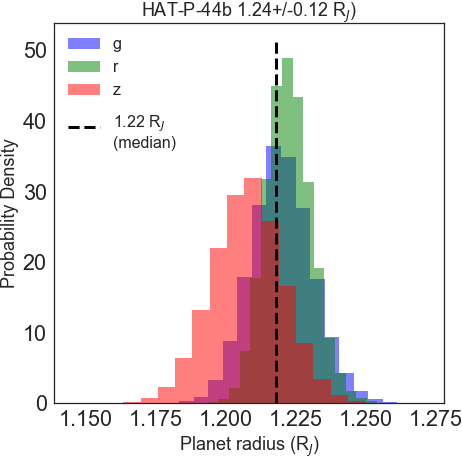
\includegraphics[width=6cm]{hatp44/radius_ratios_Rjup.png}
    \caption{Posterior distributions of Rp/Rs in each band.}
\end{subfigure}%
\begin{subfigure}{.5\textwidth}
	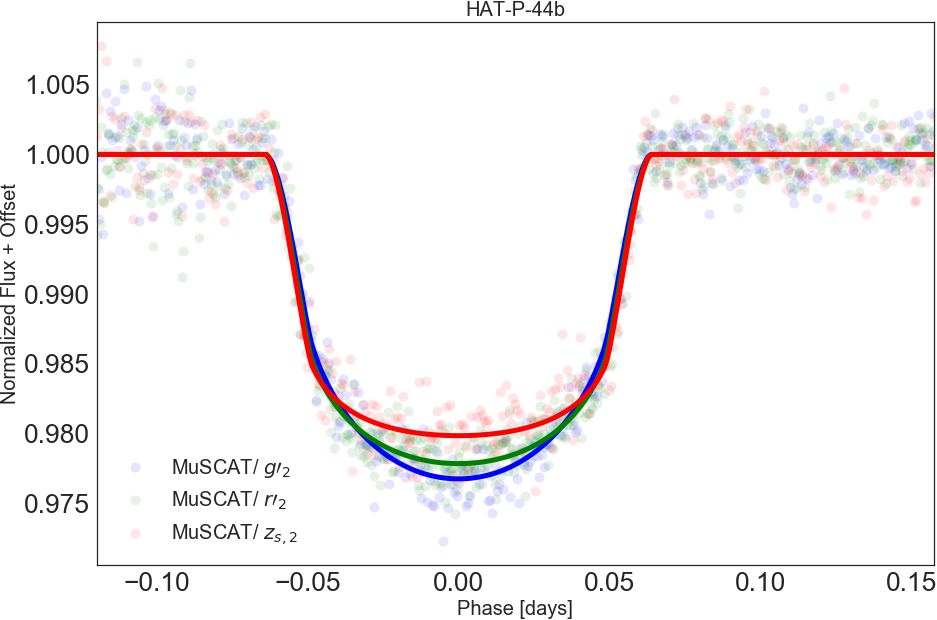
\includegraphics[width=8cm]{hatp44/grz_multi_stacked.png}
    \caption{Superposed data and best fit transit model}
    \label{fig:hatp44_stacked}
\end{subfigure}
\caption{(a) Maximum a posteriori (MAP) value of Rp/Rs in each band shows that their difference is marginal; (b) The best fit transit model (colored lines) and systematics-corrected data (colored points) are stacked compare transit depth variation.}
\label{fig:hatp44_RpRs}
\end{figure}

\begin{figure}
\centering
\begin{subfigure}{.5\textwidth}
	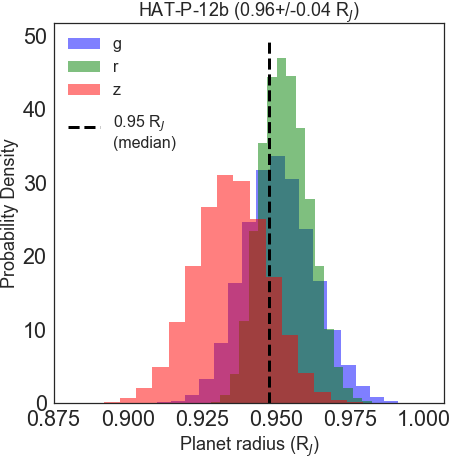
\includegraphics[width=6cm]{hatp12/radius_ratios_Rjup.png}
    \caption{Posterior distributions of Rp/Rs in each band.}
\end{subfigure}%
\begin{subfigure}{.5\textwidth}
	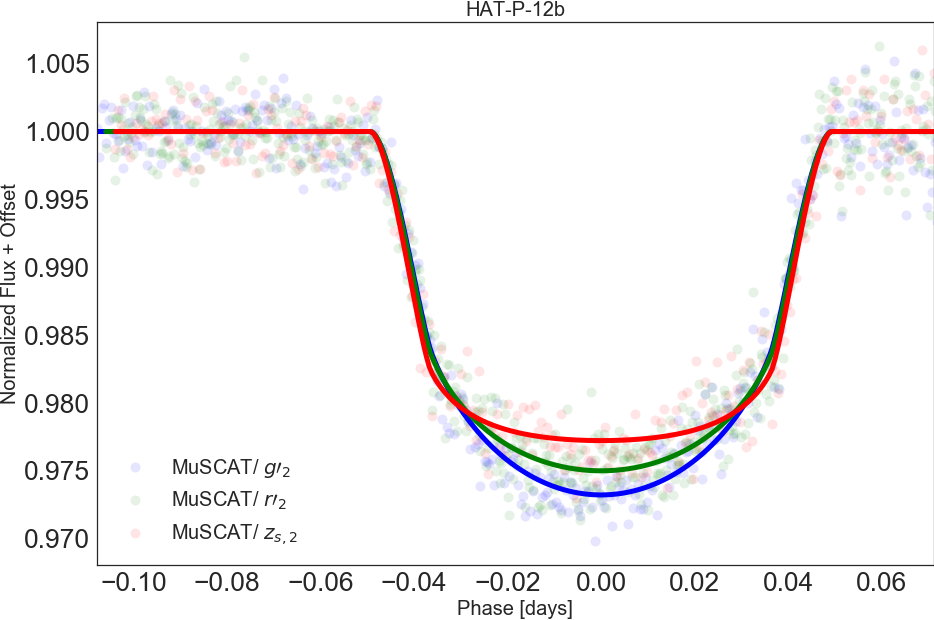
\includegraphics[width=8cm]{hatp12/grz_multi_stacked.png}
    \caption{Superposed data and best fit transit model.}
    \label{fig:hatp12_stacked}
\end{subfigure}
\caption{Same as Fig~\ref{fig:hatp44_RpRs} but for HAT-P-12b. Detection of Rp/Rs variation is also marginal.}
\label{fig:hatp12_RpRs}
\end{figure}

\begin{figure}
\centering
\begin{subfigure}{.5\textwidth}
	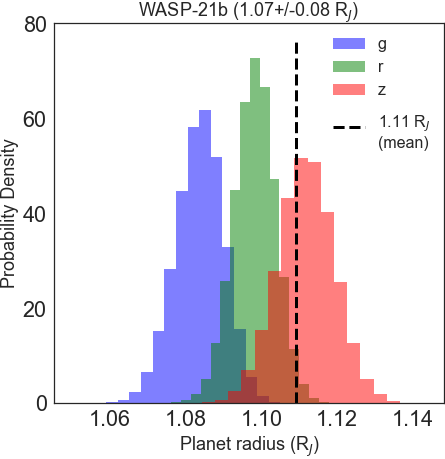
\includegraphics[width=6cm]{wasp21/radius_ratios_Rjup.png}
    \caption{Posterior distributions of Rp/Rs in each band.}
\end{subfigure}%
\begin{subfigure}{.5\textwidth}
	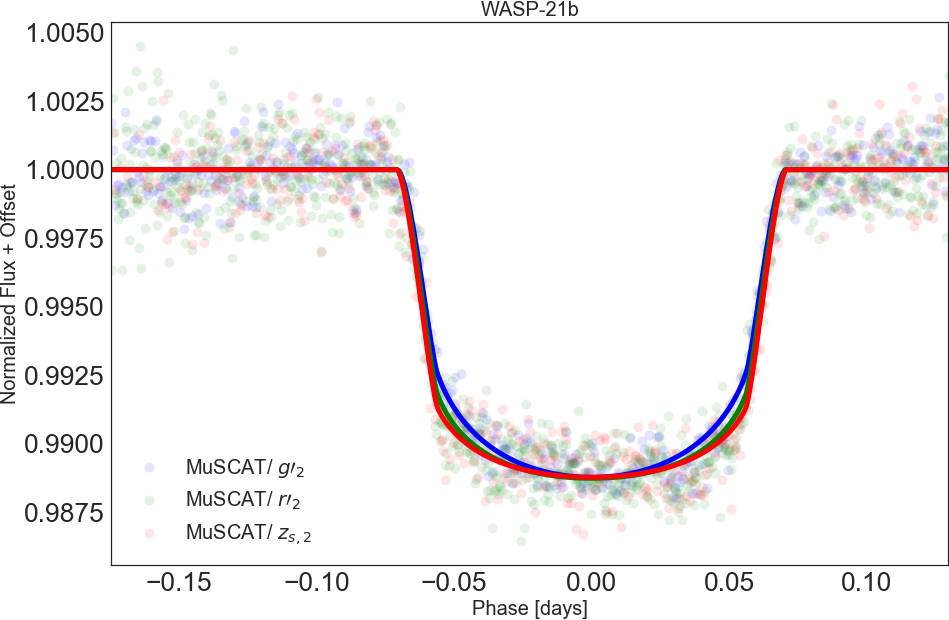
\includegraphics[width=8cm]{wasp21/grz_multi_stacked.png}
    \caption{Superposed data and best fit transit model.}
    \label{fig:wasp21_stacked}
\end{subfigure}
\caption{Same as Fig~\ref{fig:wasp21_RpRs} but for WASP-21b. Detection of Rp/Rs variation is marginal (2.8$\sigma$) and the trend is not of atmospheric origin and instead such feature is best explained by an unocculted spot on the surface of WASP-21 (see text for details).}
\label{fig:wasp21_RpRs}
\end{figure}

%------------------------------------------------------------------------
\paragraph{Empirical Scale height and Mean molecular weight}
\cite{Benneke2012} derived an equation used to estimate the scale height $H$ given Rp/Rs measurements:
\begin{equation}
\label{eq:H_emp}
H \approx \frac{R_{P,\lambda_2}-R_{P,\lambda_1}}{4 \ln \Big(\frac{\lambda_1}{\lambda_2}\Big)}
\end{equation}
given two transit depth observations at $\lambda_1 \& \lambda_2$ in the Rayleigh scattering regime. 
%show for general atmospheres that the value of the mean molecular mass can be determined by measuring the slope of the Rayleigh scattering signature at short wavelengths, dRP,λ d(lnσλ) , with which the ”observed” planet radius, RP,λ, changes as a function of the extinction cross section, σλ, across different wavelengths.

\cite{Benneke2012} also showed that the mean molecular mass $\mu$ of a general atmosphere can be estimated via
\begin{equation}
\label{eq:mu}
\mu =\frac{4k_BT}{gR_*}\frac{\ln \Big(\frac{\lambda_1}{\lambda_2}\Big)}{\Big(\frac{R_P}{R_*}\Big)_{\lambda_2} -\Big(\frac{R_P}{R_*}\Big)_{\lambda_1}} \times \Big(1\pm\frac{\delta T}{T}\Big)
\end{equation}
where $T$ is the atmospheric temperature. The factor $(1\pm \frac{\delta T}{T})$ accounts for the inherent uncertainty due to the uncertainty, $\delta T$, at the observed planet radius $r = R_{P,\lambda}$. % the mean molecular mass varies by a factor on the order of 8−20 between hydrogen-dominated atmospheres and atmospheres mainly composed of H$_2$O, N$_2$, or CO$_2$.

Table~\ref{tab:mu} summarizes our results for empirical $H$ and $\mu$ using Eq.~\ref{eq:mu} and Eq.~\ref{eq:mu} where we assumed $T\approx T_{eq}$. We used r-band as reference wavelength because of smaller uncertainty. These estimates are only valid for Rayleigh scattering regime. As apparent in Fig.~\ref{fig:wasp21_RpRs}, WASP-21b spectrum does not show apparent Rayleigh slope and hence no estimates are provided in Table~\ref{tab:mu}. For HAT-P-12b, the empirical scale height estimate ($\sim$700 km) at the empirical $\mu$=2.92 amu from the theoretical value ($\sim$500 km) by a large margin. 

%This is 
\begin{table}
\centering
\caption{Empirical estimates of scale height and mean molecular weight of the planet's atmosphere based on Rp/Rs measurements.}
\label{tab:mu}
\begin{tabular}{llllll} 
\hline
          &\multicolumn{2}{c}{$H$ (km)}& $\mu$ (amu) \\ %g (m/s$^2$) & $T_{eq}$ (K) &
          &  theoretical & empirical & & \\
\hline
HAT-P-12b & 615.6 & 765.6 & 2.88$\pm$0.5 \\ % 5.62 $\pm$ 0.01 &  963$\pm$16  &
HAT-P-44b & 708.2 & 613.6 & 5.79$\pm$0.8 \\ %& 5.62 $\pm$ 0.01 & 1108$^{+51}_{-32}$ 
WASP-21b  & 950.0 & -- &-- \\ %5.07 $\pm$ 0.035 & 1340$\pm$32   &
\hline
\end{tabular}
\end{table}

%Teq for a planet around HAT-P-14, HAT-P-11, and GJ1214 is calculated to be 1652 K, 861 K, and 398 K, respectively.
%We note that $T_{eq}$ can vary by up to $\sim15\%$ in the range of 2 < P(days) < 5 and 0 < $A$ < 0.7; however, the impact of this change on $H$ is trivial compared with that of the possible range of the surface gravity $g_p$, which extends by a factor of several or even two orders of magnitude depending on the planetary size.

%------------------------------------------------------------------------

%=======================================================================
\section{Atmospheric Models}
%Spectrum modeling is done by fitting the data with a synthetic spectrum created using best estimates of the desired atmospheric properties %(using prior knowledge and new observations), 
%such as the mixing ratios of the molecular constituents and the surface/cloud-top pressure.
We plotted the measured Rp/Rs with uncertainties as a function of wavelength (i.e. transmission spectrum) in Fig.~\ref{fig:atm_hatp44b}--\ref{fig:atm_wasp21b}. The vertical error bars correspond to measurement error and horizontal error bar correspond to the width of the bandpass of MuSCAT filters.
%The calculated model spectrum is shown as black solid line in Figure 6 where the initial model is vertically shifted such that the mean value of the model fits to the observation. Again, the expected Rp/Rs variations of this planet are too low with respect to the observational uncertainties.
In addition, to compare the observed data with a theoretical atmospheric model, we calculate a model spectrum of Rp/Rs for each planet. Detailed discussion of spectrum modeling procedure is beyond the scope of this thesis. The model description and procedure are detailed in \cite{Kawashima2015} and \cite{Kawashima2017} (see also \cite{Fukui2014}) and so we summarize the relevant information as follows.
% sensitivity of transmission spectra to the production rate of haze monomers, which relates to the amount of UV irradiation from the host star. 

%The calculation is done based on the method described in Fukui et al. (2014), but in this case line absorption of H 2 S, OCS, O 2 , TiO, and VO are taken into account in addition to those treated in Fukui et al. (2014) (H 2 , H 2 O, CH 4 , CO, CO 2 , NH 3 , N 2 , Na, and K). 
%Further, the absorption cross sections for these species are calculated on a wavelength-by-wavelength basis with a step size given by dividing the wavelength range from 0.3 to 1.0 $\mu$m by 2.5$\times$10 5 in log scale without taking the geometric mean for a  certain range of wavelengths as done in Fukui et al. (2014). An initial model spectrum is calculated by assuming that R0, the planetocentric distance at which the atmospheric pressure is 10 bar, is equal to 1.219 R Jup (Southworth 2012). 

%Theoretical Rayleigh Scattering Slope: Seager and Benneke (2012)
We calculated the spectrum models for 1 $\times$ Solar (case 1) and 100 $\times$ Solar metallicity clear atmospheres (case 2) for each exoplanet. For case 1, we consider an atmosphere with solar elemental abundances. This model atmosphere is composed of 11 elements, namely H, He, C, N, O, Na, K, P, S, Ti, and V with abundance ratios similar to those of the Solar system.% as shown in Table~\ref{tab:abundances}. 
The term metallicity means the total mass fraction of the nine elements other than H and He, with adapted value of 0.01036. For case 2, we consider a H-dominated atmosphere with metallicity enhanced by a factor of 100 relative to the solar metallicity (i.e. 1.036).
%The files without the name “smooth” is ones for the spectrum model of high resolution and ones with the name “smooth” are for the spectrum models smoothed for the clarity by averaging over the wavenumber range of 63.2 cm$^{-1}$ for each point. 
In both models, it is assumed that the atmospheres have thermochemical equilibrium compositions and isothermal structures with the equilibrium temperatures reported Table~\ref{tab:params}. %Note that MuSCAT filters do not overlap with emission lines by Na D doublet ($\sim$0.589 $\mu$m) and the potassium resonance doublet ($\sim$0.77 $\mu$m) as shown by the models.
Also, as pressure-radius relation is unknown for exoplanets, we found the appropriate value of radius at which the pressure is 10 bar that matches the theoretical spectrum with the transit radius we observed. The value of degrees of freedom (d.o.f.) is 2 for all the cases as there is 1 parameter, the value of radius at which the pressure is 10 bar. 

The data and model spectra are shown in Fig.~\ref{fig:atm_hatp12b}--\ref{fig:atm_wasp21b}. To discriminate which model is favored, the (reduced) $\chi^2$ %goodness of fit 
are computed and summarized in Table~\ref{tab:chi2}. Individual cases are discussed below.

\paragraph{HAT-P-12b}
As seen in Fig.~\ref{fig:atm_hatp12b}, the measured Rp/Rs coincide with either model because of the large uncertainties in Rp/Rs (hereby referred to as fractional uncertainties). %The measured Rp/Rs in all MuSCAT bands are consistent with the atmospheric model with $\chi^2$/dof=0.950, %$\chi^2$=28.0 and dof=2
%implying that our measured uncertainties in the individual band are underestimated. 
%Rp/Rs is not constant over the observed wavelength range within 1.8$\sigma$. 
%The larger value for (reduced) $\chi^2$ implies that the 100$\times$ Solar model is more favored.
The values of $\chi^2$ / d.o.f. are 0.217 and 0.711 for 1 $\times$ Solar and 100 $\times$ Solar atmospheres, respectively. Our photometric precision is not enough to distinguish between two models.
%We note that that our results for HAT-P-12b cannot conclusively distinguish between our two atmospheric models. 
%This is because the 1$\sigma$ uncertainties of the measured Rp/Rs is at the level of $\sim$2 times as large as one scale height (See Table~\ref{tab:H/u}). In the case of HST/STIS observations, $H/\sigma_{Rp/Rs}$ is between 0.5-2.2 scale heights in the optical wavelengths.
%can also be interpreted as consistent with a flat spectrum without the knowledge of the published HST/STIS spectra. 

\paragraph{HAT-P-44b}
%HAT-P-44b was observed by \cite{Hartmann2014} in the $r,i,I$-bands but their modeling assumed constant transit depth in all filters. 
Similar to HAT-P-12b, the measured Rp/Rs for each band coincide with either model spectrum as shown in Fig.~\ref{fig:atm_hatp44b} because of the large uncertainties. However, we achieve a smaller absolute individual fractional uncertainty, the largest among them has absolute amplitude of $\sim$0.006 for z-band. %The measured Rp/Rs in all MuSCAT bands are consistent with the atmospheric model with $\chi^2$/dof=0.950, %$\chi^2$=28.0 and dof=2
%implying that our measured uncertainties in the individual band are underestimated. 
%Rp/Rs is not constant over the observed wavelength range within 1.8$\sigma$. 
%The larger value for (reduced) $\chi^2$ implies that the 100$\times$ Solar model is more favored.
The values of $\chi^2$ / d.o.f. are 0.884 and 0.363 %0.406 and 0.151 
for 1 $\times$ Solar and 100 $\times$ Solar atmospheres, respectively. Our photometric precision is not enough to distinguish between two models.

\paragraph{WASP-21b}
Unlike HAT-P-12b and HAT-P-44b, the measured Rp/Rs do not coincide with either model spectrum except for the r-band with absolute amplitude of$\sim$0.002, as shown in Fig.~\ref{fig:atm_wasp21b}.
The values of $\chi^2$ / d.o.f. are 3.1 and 2.4 %8.00 and 4.40 
for 1 $\times$ Solar and 100 $\times$ Solar atmospheres, respectively, implying that both models cannot explain the data even with the small uncertainties. %As opposed to Rayleigh scattering feature (negative slope) in the optical wavelength, the apparent trend (positive slope) is inconsistent with our atmospheric model. We discuss the nature of this feature in \S \ref{sec:discussion}.

\begin{table}
\centering
\caption{$\chi^2$ value for both atmosphere models for each data set. The reduced $\chi^2$ is enclosed in parenthesis.}
\label{tab:chi2}
\begin{tabular}{llll}
& 1 $\times$ Solar & 100 $\times$ Solar \\
\hline
HAT-P-12b & 0.266 (0.515)  & 0.471 (0.687)  \\   
HAT-P-44b & 0.782 (0.884)  & 0.132 (0.363)  \\    
WASP-21b  & 9.978 (3.159)  & 5.660 (2.379)  \\       
%0.406)     &   (0.151)
%(8.00)  &  (4.40)
\hline
\end{tabular}
\end{table}

\begin{figure}
\centering
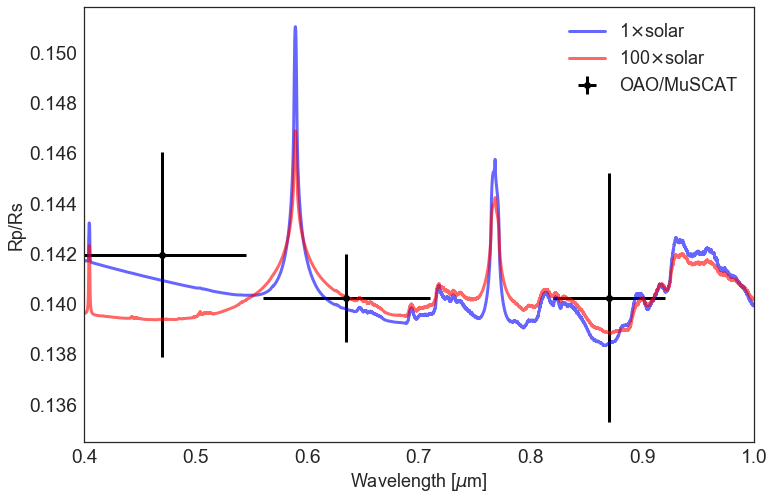
\includegraphics[width=12cm]{hatp12/atm_model.png}
\caption{HAT-P-12b transmission spectrum. From left to right, the three data points %black circle, square, and triangle 
correspond to MuSCAT g, r, and z-bands, respectively. The horizontal bars indicate the full width at half maximum of the response functions of the respective filter. Spectrum models with 1 $\times$ Solar (blue) and 100 $\times$ Solar atmospheres (green) assumes $T_{eq}$ = 963$\pm$16 K. 
 %The Rayleigh slope we observed are much steeper than the clear atmosphere models implying that haze or aerosol may exist in the atmosphere. 
 The values of $\chi^2$ / d.o.f. are 0.52 and 0.69 for 1 $\times$ Solar and 100 $\times$ Solar atmospheres, respectively, implying that our photometric precision is not enough to distinguish between two models.
 }
\label{fig:atm_hatp12b}
\end{figure}

\begin{figure}
\centering
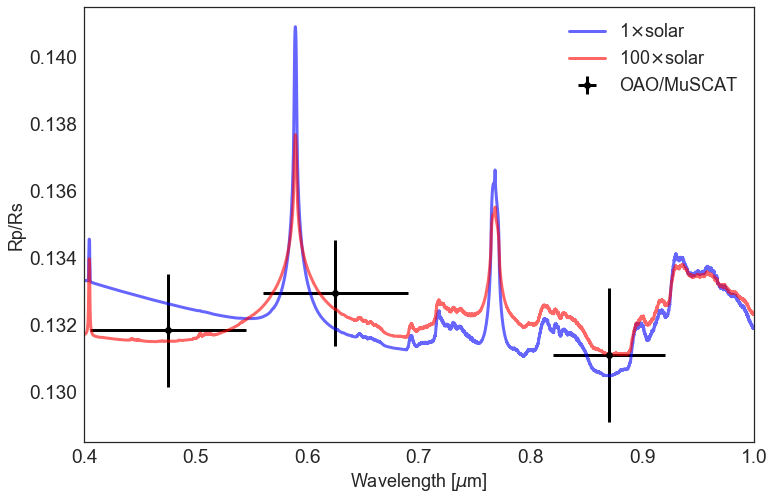
\includegraphics[width=12cm]{hatp44/atm_model.png}
\caption{Same as Fig~\ref{fig:atm_hatp12b} but for HAT-P-12b assuming $T_{eq}$ = 963$\pm$16 K. 
The values of $\chi^2$ / d.o.f. are 0.88 and 0.36 for 1 $\times$ Solar and 100 $\times$ Solar atmospheres, respectively, implying that our photometric precision is not enough to distinguish between two models.}
\label{fig:atm_hatp44b}
\end{figure}

\begin{figure}
\centering
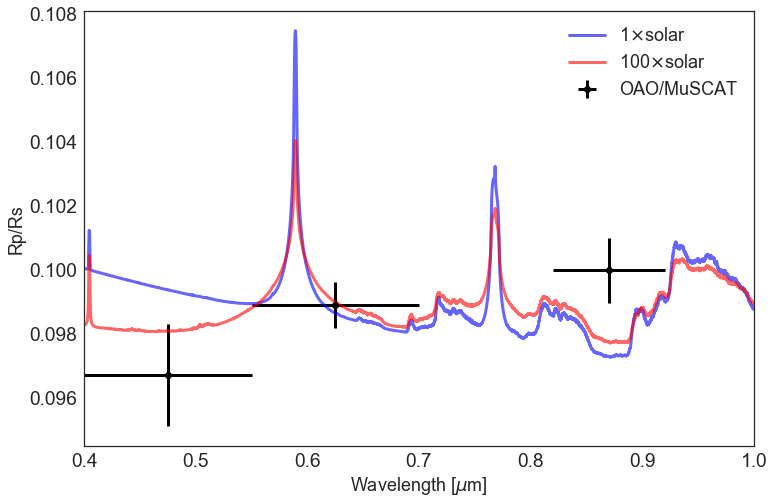
\includegraphics[width=12cm]{wasp21/atm_model.png}
\caption{Same as Fig~\ref{fig:atm_hatp12b} for WASP-21b but assuming $T_{eq}$ = 1340$\pm$32 K. The values of $\chi^2$ / d.o.f. are 3.2 and 2.4 for 1 $\times$ Solar and 100 $\times$ Solar atmospheres, respectively, implying that the data cannot be explained by either model.}
\label{fig:atm_wasp21b}
\end{figure}


\begin{comment}
The calculation is done based on the method described in Fukui et al. (2014), but in this case line absorption of H2S, OCS, O2, TiO, and VO are taken into account in addition to those treated in Fukui et al. (2014) (H2, H2O, CH4, CO, CO2, NH3, N2, Na, and K). 

Further, the absorption cross sections for these species are calculated on a wavelength-by-wavelength basis with a step size given by dividing the wavelength range from 0.3 to 1.0 μm by ∼2.5e5 in log scale without taking the geometric mean for a certain range of wavelengths as done in Fukui et al. (2014). An initial model spectrum is calculated by assuming that R0, the planetocentric distance at which the atmospheric pressure is 10
bar, is equal to 1.219 RJup (Southworth 2012).

Again, the observed Rp/Rs variations of this planet are too low with respect to the
observational uncertainties. 
\end{comment}
%---Discussion
\chapter{Discussion}\label{sec:discussion}
\section{Rayleigh Scattering Slope}
\paragraph{HAT-P-12b}
For HAT-P-12b, we use additional high precision data from \cite{Sing2016}\footnote{Data downloaded from http://www.astro.ex.ac.uk/people/sing/spectra/?/people/sing/spectra/HAT-P-12b} using HST/STIS in the optical wavelengths (see \S \ref{sec:followup}). As shown in Fig.~\ref{fig:hatp12_sing}, the measured Rp/Rs (black) in MuSCAT g-,r-,and z-bands are superposed with the data (magenta) and atmospheric model (green line) of \cite{Sing2016}. Fitting our measurement with this model yields a $\chi^2$/ d.o.f.= 0.316 implying overestimated uncertainties. %This confirms that the observed trend is consistent with the previous result.
%Using HST data alone, $\chi^2$/dof=0.998
%Using HST+MuSCAT data, $\chi^2$/dof=0.950
Although our achieved (1 $\sigma$) uncertainties for Rp/Rs are only about 2$\times$ to 5$\times$ to that in \cite{Sing2016}, we note that that our results for HAT-P-12b cannot conclusively distinguish between our two atmospheric models. To distinguish between our two models however, we only need an improvement 1.5$\times$ photometric precision in g-band.
This is because the 1$\sigma$ fractional uncertainties of the measured Rp/Rs is at the level of $\sim$2 times as large as one scale height (See Table~\ref{tab:H/u}). In the case of HST/STIS observations, the fractional uncertainties %$H/\sigma_{Rp/Rs}$ 
are between 0.5-2.2 scale heights in the optical wavelengths.
In any case, this confirms the validity of our transit modeling approach that %correctly measured the predicted radius variation of HAT-P-12b at the wavelengths relevant for our observation. 
produce measurements that do not significantly deviate from the theoretical Rayleigh slope.
%can also be interpreted as consistent with a flat spectrum without the knowledge of the published HST/STIS spectra. 

%\paragraph{HAT-P-44b}

\begin{figure}
\centering
	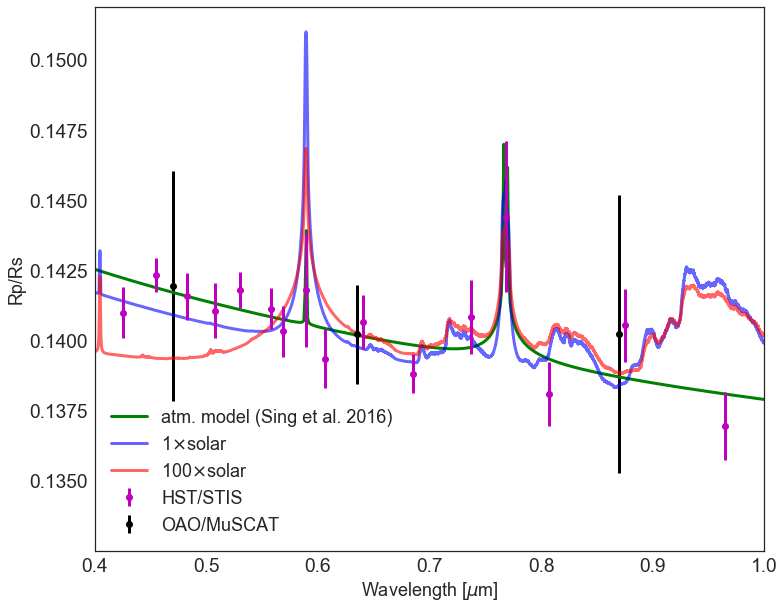
\includegraphics[width=10cm]{hatp12/atm_model_full.png}
    \caption{Transmission spectrum of HAT-P-12b. The measured Rp/Rs using MuSCAT in g-,r-,and z-bands (red points) are superposed with the data (blue points) and atmospheric model (green line) of \cite{Sing2016}. The vertical lines represent 1-$\sigma$ uncertainties.
    }\label{fig:hatp12_sing}
\end{figure}

\paragraph{WASP-21b}
As shown in Table~\ref{tab:wasp21_map}, we found a %mean variation 
difference of $\sim$0.3\%  in the transit depth of WASP-21b %09670, 0.09889, 0.09998
between z- and g-bands which is greater than the uncertainties. 
As opposed to Rayleigh scattering feature (negative slope) in the optical wavelength, the apparent trend (positive slope) is inconsistent with our atmospheric model. 
%Archival data of WASP-21b\footnote{http://var2.astro.cz/ETD/etd.php?STARNAME=HAT-P-21&PLANET=b} show a transit depth variability semi-amplitude of at most 7 mmag in R-band. %and 5 mmag in clear band.  
To confirm that this feature is inherent in the data and not due to our modeling, we re-analyze each light curve independently. We show in Fig.~\ref{fig:wasp21_combined_grz} that the result is consistent with increasing transit depths towards shorter wavelengths. 

As stellar activity can affect the measurement of a transmission spectrum, we %photometrically monitored 
check the activity levels of WASP-21 by analyzing archival data from ETD.\footnote{} 
WASP-21 shows low levels of stellar activity, with observed photometric variations or upper limits which are sufficiently small that their effects on measuring the transmission spectra are minimal compared to the measurement errors3,4,11–13. %We try to were corrected for occulted and un-occulted star spots10,14. 
We reserve the discussion of the nature of this trend in \S \ref{sec:spots}.

\begin{figure}
\centering
	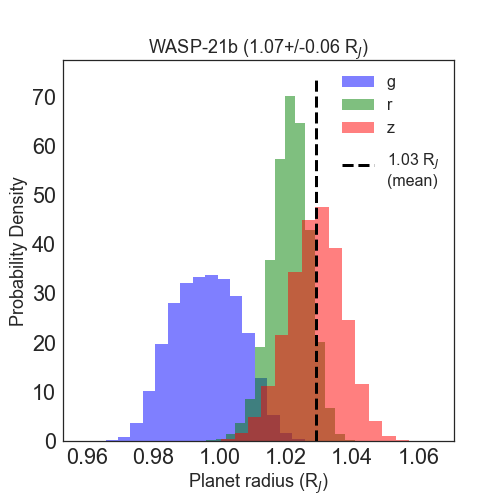
\includegraphics[width=8cm]{wasp21/radius_ratios_Rjup_per_band.png}
    \caption{Posterior distribution of Rp/Rs obtained from independent (i.e. per color) re-analysis of WASP-21 light curve showing trend consistent with simultaneous, multi-color modeling.}
    \label{fig:wasp21_combined_grz}
\end{figure}

%Finally, we search for Rp/Rs variations with wavelength, which can in principle be observed due to the atmospheric opacity variations. %The measured Rp/Rs values and their uncertainties in respective bands are listed in Table 6 and shown in Figure 6. 
%A constant fit to these values gives the mean value of Rp/Rs = 0.08179  0.00064 with c2 = 13.0 for dof=6, meaning that Rp/Rs is constant over the observed wavelength range within 2$\sigma$. 

\section{Significance of Detection}
%In the following, we aim to determine whether the measured Rp/Rs in all bands are constant or consistent with a Rayleigh slope over the observed wavelength range. 
To evaluate the robustness of our detection, we did a Monte Carlo simulation in which we sample from the posterior distribution of Rp/Rs of each band and computed the Rayleigh slope. The distribution of slope and intercept are shown in Fig.~\ref{fig:hatp12_slope}--Fig.~\ref{fig:wasp21_slope}. The dashed red and blue line correspond to Rayleigh scattering slope expected for 1 Solar and 100 Solar atmosphere model, respectively. The mean of the slope distribution is biased away from the dotted black line by at least 1$\sigma$. In other words, all the data set cannot be explained by a flat spectrum. Even though both HAT-P-12b and HAT-P-44b spectra is consistent with a Rayleigh slope in the optical, our detections are marginal. 
%Equivalently, the mean of the slope distribution is consistent with the predicted theoretical Rayleigh slopes. 
However, the measured uncertainty (width of the slope distribution) is not small enough to distinguish between two atmospheric models as also evident in the model spectra.

Following \cite{Fukui2016a}, we estimate how sensitive these Rp/Rs measurements are to atmospheric signatures by comparing the estimated 1-$\sigma$ measurement error of Rp/Rs, $\sigma_{Rp/Rs}$, with the expected variation
of Rp/Rs due to the atmospheric effect. When a planet has an atmosphere with no thick clouds, Rp/Rs can vary with wavelength by up to several H/Rs. Therefore, if $\sigma_{Rp/Rs}$ is comparable to or smaller than the expected value of H/Rs, it can roughly be considered that the measurement is sensitive to the atmosphere. Based on Fig.~\ref{fig:HRs-sigRpRs}, our achieved precision is enough to detect atmospheric features but only for the case of WASP-21b.

\begin{figure}
\centering
	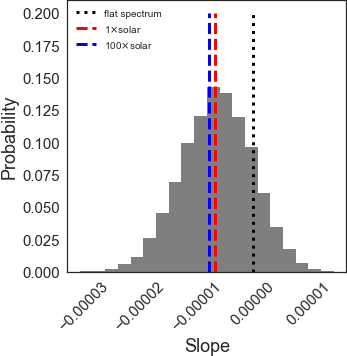
\includegraphics[width=8cm]{hatp12/slope.png}
    \caption{Monte Carlo simulation of fitting a straight line to the measured Rp/Rs by directly sampling from the posterior distribution. The red and blue vertical lines correspond to the expected slope for a 1$\times$ and 100$\times$ Solar atmosphere while the black line correspond to zero slope (i.e. flat spectrum). The mean slope is consistent with the expected Rayleigh slope and biased away from zero within 1.8$\sigma$.
    }\label{fig:hatp12_slope}
\end{figure}

\begin{figure}
\centering
	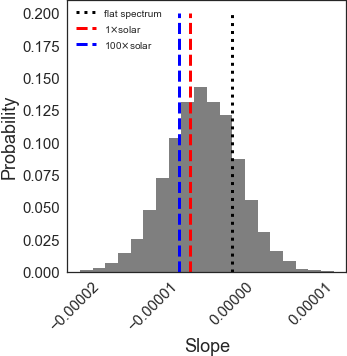
\includegraphics[width=8cm]{hatp44/slope.png}
    \caption{Same as in \ref{fig:hatp12_slope} but for HAT-P-P-12b. The mean slope is biased away from zero by 1.0$\sigma$.
    }\label{fig:hatp44_slope}
\end{figure}

\begin{figure}
\centering
	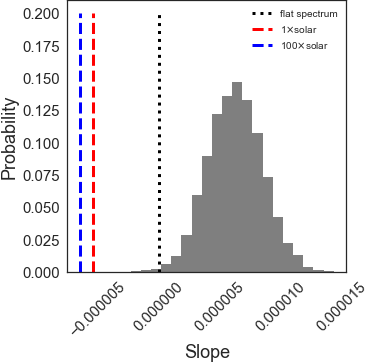
\includegraphics[width=8cm]{wasp21/slope.png}
    \caption{Same as in \ref{fig:hatp12_slope} but for WASP-21b. A positive slope is cannot be attributed to Rayleigh scattering. The mean slope is biased away from zero by 2.8$\sigma$.
    }\label{fig:wasp21_slope}
\end{figure}

\begin{table}
\centering
\caption{Required improvement in photometric precision to be sensitive to atmospheric features (See also Fig.~\ref{fig:HRs-sigRpRs}). Only z-band of WASP-21b is sensitive to detection of expected atmospheric feature.}
\begin{tabular}{lll}
\label{tab:H/u}
                  & & $\sigma_{Rp/Rs}/H/Rs$ \\ \hline                     
 \multirow{3}{*}{HAT-P-12b}& g-band:& 1.96 $\pm$ 0.19  \\
                           & r-band:& 1.44 $\pm$ 0.14  \\
                           & z-band:& 2.73 $\pm$ 0.26  \\ \hline
 \multirow{3}{*}{HAT-P-44b}& g-band:& 1.93 $\pm$ 0.06  \\
                           & r-band:& 1.80 $\pm$ 0.05  \\
                           & z-band:& 2.67 $\pm$ 0.08  \\ \hline
 \multirow{3}{*}{WASP-21b} & g-band:& 1.22 $\pm$ 0.06  \\
                           & r-band:& 1.05 $\pm$ 0.05   \\
                           & z-band:& 0.97 $\pm$ 0.05  \\
\hline
\end{tabular}
\end{table}

\begin{figure}
\centering
	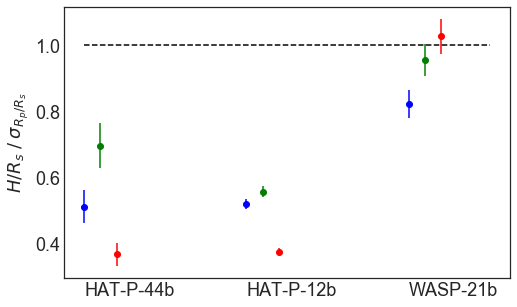
\includegraphics[width=10cm]{figures/H-sigRpRs.png}
    \caption{Measured sensitivity of Rp/Rs measurements to atmospheric signatures. $\sigma_{Rp/Rs}/H/Rs$>1 implies robust detection.}\label{fig:HRs-sigRpRs}
\end{figure}

%Note that optical and infrared data are both crucial for this claim of "cloudiness" because the measurement of a Rayleigh signal in the optical alone is not sufficient as it could be simply caused by H2 and He. Only a spectral slope less negative than −4 in the optical may allow us to infer the presence of large particle (a$\geq \lambda/2 \pi$) clouds from the spectrum alone, but this requires an accurate estimate of the atmospheric scale height (Heng 2016).

%In order to further explore the notion that the combination of individual light curves does tend to cancel out systematic errors present in the original data we have created Allan variance plots of the residuals (observed minus model) corresponding to each of the individual light curves and the residuals corresponding to the resulting combined light curves. For this, we followed the formalism detailed in Carter et al. (2009). We have used their definition of Allan variance as stated in their Equation (8) to plot its value as a function of lag. This is shown

\section{The Case of WASP-21b: Unocculted Star Spot} \label{sec:spots}
%However, best-fit model does not show apparent difference in transit depth among different filters. Is it because of sampling only? No! I checked that samples do show difference.
The apparent increase in transit depth towards longer wavelengths is not consistent with an atmospheric model including Rayleigh scattering in the optical as shown in Fig.~\ref{fig:atm_wasp21b}. Instead, this trend is consistent with unocculted starspots that may be present on the surface of the star but are not along the transit chord (i.e. different from a spot-crossing event e.g. \cite{Pont2008}). %unocculted spots mimic Rayleigh scattering in transmission spectrum (McCullough+2014; Oshagh+2014)
%After taking into account the overall flux level of the star and implementing a wavelength-dependent radius correction assuming a reasonable spot temperature, Pont+2008 and Sing+2011 attribute this effect to be of atmospheric origin and not stellar spots

Unocculted starspots are known to cause a systematic effect on the apparent Rp/Rs due to chromatic abberations and rotational modulations (see e.g., Carter et al. 2011; Désert et al. 2011b; Sing et al. 2011). 
These unocculted spots can be accounted for by a wavelength-dependent depth correction. As with \cite{Narita2013}, %Kirk+2016, 
we follow the formalism of \cite{Sing2011} to make this correction. %We use \verb'ATLAS9' stellar models (\cite{Kurucz1993}) of a star with temperature $T_{star}$ = 5800 K for WASP-21 and spot temperatures with temperature difference $\Delta T$ ranging from 250 K to 1250 K. Using this variation, we assume a total dimming 0.4\% at reference wavelength of 600 nm and use equations (4) and (5) in \cite{Sing2011} to find the correction in Rp/Rs across the wavelength range spanned by MuSCAT g- and z-bands (400-920 nm). %We find that the effect of spots on this star is large as they lead to a correction in Rp/Rs of between X and X which is comparable to the 1-sigma error bars of our measured Rp/Rs in MuSCAT data.
The systematic difference of the radius ratio $\Delta(R_p/R_s)$ caused by the stellar variability due to starspots can be written as
\begin{equation}
 \Delta(R_p/R_s) \simeq 0.5 \Delta f(\lambda) R_p/R_s
\end{equation}
where  $\Delta f(\lambda)$ is the stellar brightness variability at wavelength $\lambda$. 
Assuming the black-body profile for the emission from those regions, we search for an optimal spot coverage that can explain the semi-amplitude of g- and z-band variability. We find that a spot coverage of 0.5\% gives the best-fit for those two bands. This shows that our atmospheric modeling is useful to categorically rule out the possibility that the observed trend in WASP-21b spectrum is atmospheric in origin. 


\section{Selecting Future Targets for MuSCAT \label{sec:targetselection}}
The amplitude of the absorption within the exoplanet's atmosphere can be approximated as (e.g. \cite{Encrenaz2014})
\begin{equation}
A=10\frac{H}{R_s}\frac{R_p}{R_s}
\end{equation}

Thus, the critical property of a target when performing transit spectroscopy is the relative size of the planet to its star. This makes the atmospheres of large gas giants generally much easier to recover. Similarly, smaller planets around dwarf hosts are favorable. %55 Cnc e (Demory et al. 2011; Winn et al. 2011; V=5.95) and HD 97658b (Dragomir et al. 2013; V=7.7). 
However, only very few of these small targets are bright enough for atmospheric characterization from the ground. 

Table~\ref{tab:A} shows currently known targets with host brighter than m$_v$=13.5 and ranked in increasing amplitude for a Jovian, Neptunian, and terran-type exoplanet. At the time of writing, a few new targets joined the list including WASP-107, WASP-127 and EPIC 220674823/K2-106 which are being considered for proposal for MuSCAT. 

\begin{table}
\centering
\caption{Short-list of top 5 Jovian, Neptunian, and Terran transiting system ranked in decreasing $A$ signature.} 
\begin{tabular}{llllllll}
hostname	&	Vmag	&	$R_p$	&	$T_{eq}$	&	$R_s$	&	$T_{eff}$	&	$A [\%]$& Status	\\ 
\hline
Jovian (0.5 <R [R$_J$]<13)\\
\hline 
WASP-107	&	11.471	&	0.94	&	770	&	0.66	&	4430	&	0.103605	 & Proposed\\
WASP-17	&	11.6	&	1.991	&	1771	&	1.57	&	6650	&	0.098804	&  well-known\\
WASP-127	&	10.15	&	1.37	&	1400	&	1.39	&	5620	&	0.087652	& candidate \\
WASP-52	&	12	&	1.27	&	1315	&	0.79	&	5000	&	0.079451	& well-known \\
WASP-79	&	10.1	&	2.09	&	1900	&	1.53	&	6600	&	0.069718	& well-known \\ 
\hline
Neptunian	(0.35 <R [R$_J$]<0.5)	\\
\hline
K2-32	&	12.31	&	0.458	&	817	&	0.84	&	5275	&	0.018146	& candidate \\
HAT-P-11	&	9.472	&	0.422	&	878	&	0.75	&	4780	&	0.012263	& well-known \\
K2-27	&	12.64	&	0.4	&	902	&	0.89	&	5248	&	0.006348	& candidate \\
KOI-94/ Kepler-89	&	12.205	&	0.385	&	1012	&	1.52	&	6182	&	0.00432	& well-known \\
Kepler-4	&	12.7	&	0.357	&	1650	&	1.49	&	5857	&	0.003719	& well-known\\
\hline
Terran (R$_p$[R$_J$]<0.35) \\
\hline
GJ 1132	&	13.49	&	0.128	&	644	&	0.26	&	-	&	0.032978	& well-known \\
Kepler-78	&	11.551	&	0.105	&	2250	&	0.74	&	5058	&	0.006713	& well-known \\
EPIC 220674823/ K2-106	&	12.102	&	0.247	&	722	&	0.95	&	5496	&	0.005693	& well-known\\
K2-18	&	13.496	&	0.212	&	235	&	0.41	&	3457	&	0.004505	& well-known \\
Kepler-36	&	11.866	&	0.328	&	928	&	1.63	&	5911	&	0.010561	& well-known\\
\hline
\label{tab:A}
\end{tabular}
\end{table}

%To accurately detect wavelength dependent radius variation as a proxy for detecting Rayleigh scattering feature, however, photometric precision must achieve at least equal to the order of $H/R_s$.

%Because of the degeneracy between planets with high mean molecular weight atmosphere and those with high-altitude clouds or hazes %Miller-Ricci et al. 2009; Kreidberg et al. 2014) 
%optical transmission spectrum with Rayleigh scattering feature should be complemented with infrared spectrum. In such a case, observing a flat spectrum in the infrared proves that Rayleigh scattering feature detected in the optical constrains the existence of high-altitude clouds or hazes in the atmosphere.

\begin{comment}
estimates of S/N ratio for an 8 m telescope. The SINFONI/VLT time calculator is used in the K band, with an exposure time of 3 h and a resolving power of 4000. Note that the time calculator only takes into account the photon noise and assumes a perfect stability of the instrument and atmosphere, which is an optimistic assumption.

For a hydrogen-helium (H-He)-rich planet with $\mu$=2.4, the scale height can be expressed as
\begin{equation}
H=3.46\frac{T}{g}
\end{equation}
in metric units. The (surface) gravity $g$ can be expressed as
\begin{equation}
g=25\frac{M_p}{R^2_p}
\end{equation}
where $M_P$ and $R_P$ are the mass and the radius of the planet, expressed in Jovian masses and radii, respectively. Thus, the amplitude of the absorption can be written as
\begin{equation}
A=1.4\times 10^{-6}\frac{HR_p}{R^2_s}
\end{equation}
For hot Jupiters, typical values of $A$ are a few 10$^{-4}$. $A$ signature is especially strong for planets having a high temperature (and thus being close to their stars), a large radius and a low molecular weight. Inflated hot Jupiters are thus privileged targets for primary transits.
%Infrared spectroscopy of exoplanets: observational constraints
\end{comment}



\begin{comment}
%To accurately detect wavelength dependent radius variation as a proxy for detecting Rayleigh scattering feature, we search for transiting systems that have the lowest $H/R_s$. 
To select future targets amenable for future atmospheric characterization with MuSCAT, we compute $H/R_s$ for all known transiting exoplanets with well known $R_p$ and $R_s$. As seen in Eq\ref{eq:H}, scale height is a function of equilibrium temperature of the planet which is usually unknown a priori.
%First, we download the data available from NASA Exoplanet Archive \footnote{ https://exoplanetarchive.ipac.caltech.edu }. 
To estimate $H$ we first calculate the equilibrium surface temperature $T_{eq}(a,d)$ and surface gravity, $g_p(R_p,M_p)$ of the planet whenever empirical values are unavailable, and assume a fiducial mean molecular weight of $\mu$ = 2.3 for H-He dominated atmospheres. %The computed $H/R_s$ are summarized in Table~XX.%\ref{tab:future_targets}.
The plot is shown in Fig.~\ref{fig:future.png}.



%Fukui+2014a

The detectability of planetary atmospheric features through
the transmission spectrophotometry depends on how precisely
the Rp Rs value can be measured with respect to the expected
atmospheric scale height of the planet. For planning future
observations with MuSCAT, it is worthwhile investigating
what types of planet can be targeted by this instrument for the
atmospheric study.

To this end, we simulate the achievable measurement error
of Rp Rs with MuSCAT for planets with a range of sizes
around three types of host stars: 

the V = 10 F-dwarf HAT-P-14, 
the nearby (38 pc) K-dwarf HAT-P-11 (Bakos et al. 2010), and 
the nearby (14 pc) M-dwarf GJ1214 (Charbonneau et al. 2009). 

The properties of the respective stars are listed in Table 7. 

Spec. Type F5V K4V M4.5V
Radius (R) 1.59 0.683 0.211
Teff (K) 6600 4780 3026
Distance (pc) 205 38 14.3
g¢ 10.18 9.97a 15.58b
r¢ 9.94 9.16a 14.08b
z¢ 10.30 8.79a 11.86b


In each case we simulate that the host star has the
same size and brightness with the assumed star. The simulation
procedure is as follows. First we create a mock OOT light
curve for each star and each band from the residual light curve
in the same band of HAT-P-14b (see Figure 2). For mock OOT
light curves of HAT-P-14 we use the residual light curves as
they are. On the other hand, for HAT-P-11 and GJ1214 we
assume that all the conditions except for the brightness of the
host star (scintillation noise, photon noises from comparison
stars, sky background noise, and systematic noises) are the
same as those in the case of HAT-P-14, and set the error bar of
each data point in the mock OOT light curve by modifying the
error bar in the residual light curve as

\begin{figure}
\centering
	\includegraphics[width=7cm]{figures/future.png}
    \caption{Feasible targets amenable for .}
\label{fig:hatp12_tdv}
\end{figure}
\end{comment}









%---Summary, Conclusions, Future Work
\chapter{Summary, Conclusions, and Future Work \label{sec:summary}}
%observing low density super Neptunes
In this we thesis, I presented simultaneous multi-color (g-,r-, and z-bands) transit observations of low density hot Jupiters, namely HAT-P-44b, HAT-12b, and WASP-21b, using the MuSCAT instrument. %Simultaneous observation in 
The goal was to improve our understanding of these systems by refining transit parameters and searching for broad atmospheric signatures such as Rayleigh scattering in the optical wavelengths for the first time towards these systems. 

In Chapter \ref{sec:intro} a general overview of transit observation of hot Jupiters and the need for follow-up of these systems. In Chapter \ref{sec:obs} the observation and the transit modeling are discussed in detail. For the transit analysis, a Bayesian approach is implemented to model transit light curves in all bands simultaneously including wavelength-dependent systematics. This approach is useful in incorporating prior information that properly takes into account the uncertainties in the resulting best-fit transit parameters.
%results
In Chapter \ref{sec:results}, the results of transit modeling are presented which are in general agreement with previous results. % improvement in transit ephemeris. 
Careful analysis of transit depth variation in each band show a marked increase in the planetary radius from the red toward the blue ends of the visible wavelength range. For HAT-P-12b and HAT-P-44b, the measured transit depths in $g$-band have a larger Rp/Rs value than the $r$-band. Archival data using HST/STIS was used to confirm that the results of transit modeling is consistent with the accepted model spectrum for HAT-P-12b.

In Chapter \ref{sec:discussion}, spectrum model calculation for each exoplanet are presented considering two cases: (case 1) 1 $\times$ Solar and (case 2) 100 $\times$ Solar metallicity clear atmospheres, assuming thermochemical equilibrium compositions and isothermal structures. Comparing the measured transit depths with the spectrum model for HAT-P-12b and HAT-P-44b help rule out stellar activity and site-specific systematics as the source of this variation. 
To test the significance of (non-)detection of Rayleigh slope, a Monte Carlo fitting routine was performed to compute slopes directly from marginalized the transit depth distributions for each band. Results show that Rayleigh slope detection is marginal (1.5$\sigma$) for HAT-P-12b and (1.8$\sigma$) HAT-P-44b implying that the achieved photometric precision is not enough to robustly distinguish between the two atmospheric models. %Assuming that detection is true, we provide an estimate of the atmospheric scale height and the atmosphere's mean molecular weight.
However, our modeling is useful to categorically rule out the possibility that the observed trend in WASP-21b spectrum is not atmospheric in origin. Instead, the observed trend can be explained by unocculted spots on the surface of WASP-21 with a spot coverage of 0.5\%. Motivated by our results, we search for new targets feasible for future observation aimed at detecting broad atmospheric features. The new targets identified, including WASP-107, have already been considered for future observation.

%conclusion
%We conclude that the rise toward the blue end of the transmission spectrum of HAT-P-12b is due to an increase in the planetary radius, indicative of Rayleigh scattering in the planet’s atmosphere. In light of previous observations in other wavelengths, it is possible to distinguish between a H/He-dominated atmosphere covered by high-altitude clouds and hazes, which obscure absorption features in the near-IR but give rise to a steep Rayleigh scattering slope in the visible, respectively.

%Unfortunately, our achieved photometric precision is not sufficient to distinguish whether the atmosphere of HAT-P-44b and HAT-P12b can be explained by either a 1-or 100-solar metallicity abundance. 

Nevertheless, the existing data set does not constrain the atmospheric composition of HAT-P-44b beyond indicating a low-metallicity atmosphere. One way forward is through additional transit spectroscopy observations in the near- and mid-infrared, where the absorption features expected from water and carbon molecules may be detected as long as any clouds are at sufficiently low altitude. If with more precise measurements the spectrum remains featureless in this wavelength range, this would confirm the presence of haze high in the atmosphere, but would also limit the chances of further constraining this planet’s atmospheric composition.

%Our study illustrates how ground-based observations with a two-meter class telescope can provide broadband transmission spectra capable of probing atmospheric properties of exoplanets larger than super-Earths.

%The relatively quick means of planet validation and characterization using multi-color photometry has proven to be very powerful method for studying interesting transiting exoplanets during the Kepler/K2 era. This technique will be fruitful especially in the forthcoming Transiting Exoplanet Survey Satellite TESS (Ricker et al. 2015), for which MuSCAT and other ground-based transit follow-up observatories are laying the groundwork. 
 
%future work
%This study presents a continuous work to characterize transiting exoplanet systems.
The analysis employed in this work will be very useful for the near future studies of observing broad atmospheric features in exoplanet atmospheres  including Rayleigh scattering signature using a newer instrument called MuSCAT2. MuSCAT2 underwent its first light observation in late 2017 (Narita et al., in prep) and is currently conducting intensive follow-up studies of interesting transiting systems including a search for Rayleigh scattering signature. 

In addition to MuSCAT2’s improved capabilities than MuSCAT and better observing conditions in Spain, its operation is timely with the launch of the Transiting Exoplanet Survey Satellite (TESS). Unlike Kepler/K2 however, TESS will conduct all-sky survey of transiting planets around bright and nearby stars (Ricker et al. 2015). TESS is expected to discover about 300 planets smaller than 2 Earth-radii, of which 165 planets are orbiting M dwarfs and about 20 planets are orbiting the HZ (Sullivan et al. 2015). Thus,  there is a very high prospect for MuSCAT2 to become a leading facility dedicated for follow-up transit observations of new interesting planets. The multi-color transit modeling developed in this work is useful for the future studies studies related with MuSCAT2.

\chapter{Acknowledgements}
%Tamura-sensei
%John Livingston
%Yui Kawashima
%Norio Narita
%Akihiko Fukui
%insightful discussion with Stevanus
I would like to express deep gratitude to my advisers Motohide Tamura and Norio Narita for over-all support and guidance. Special thanks also to John Livingston for motivating me to work on this study and Akihiko Fukui for giving assistance during observation and suggestions during data analysis. Finally, I would like to thank Yui Kawashima for for fruitful discussions and assistance in transmission spectrum modeling used in this work. %I also thank the panel for his/her careful reading and constructive comments, which helped improve this thesis. 

%%%%%%%%%%%%%%%%%%%%%%%%%%%%%%%%%%%%%%%%%%---Appendix
\appendix
%\renewcommand\thefigure{\thechapter.\arabic{figure}}  

\chapter{Supporting Figures}
%\paragraph{Posterior Samples and Summary statistics}
%\setcounter{figure}{0}

\begin{comment}
\begin{table}
\centering
\label{tab:hatp44_summary}
\begin{tabular}{lll}
\hline
d && \\
\hline
\end{tabular}
\end{table}
\end{comment}

%Note that the joint posterior distribution directly show correlations among variables. We confirm that indeed no such correlations exist between limb darkening parameters $q_1$ and $q_2$ as shown by their posterior distributions

\begin{figure}
\centering
\begin{subfigure}{.5\textwidth}
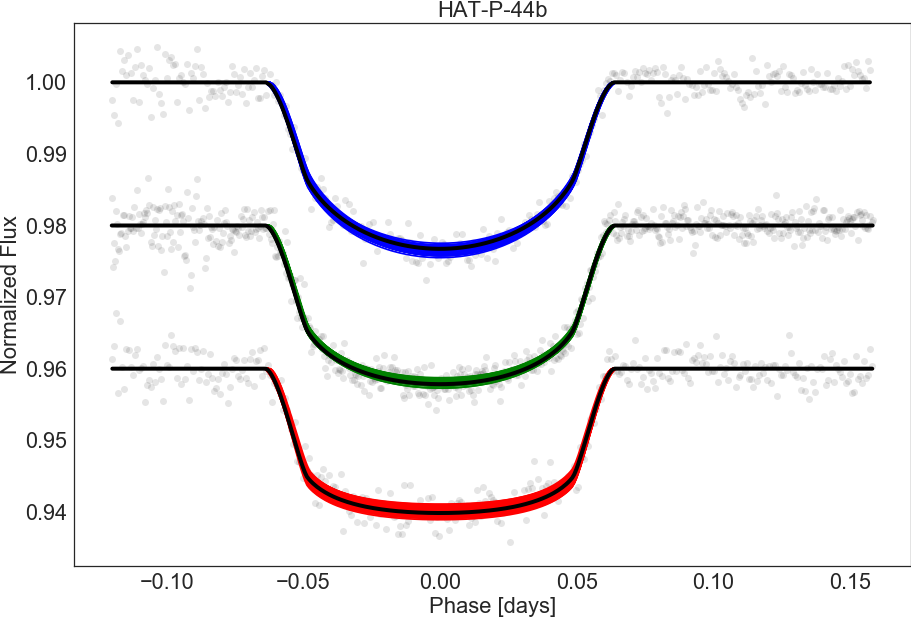
\includegraphics[width=7cm]{hatp44/1000_posterior_samples.png}
\caption{Full best-fit transit models.}
\end{subfigure}%
\begin{subfigure}{.5\textwidth}
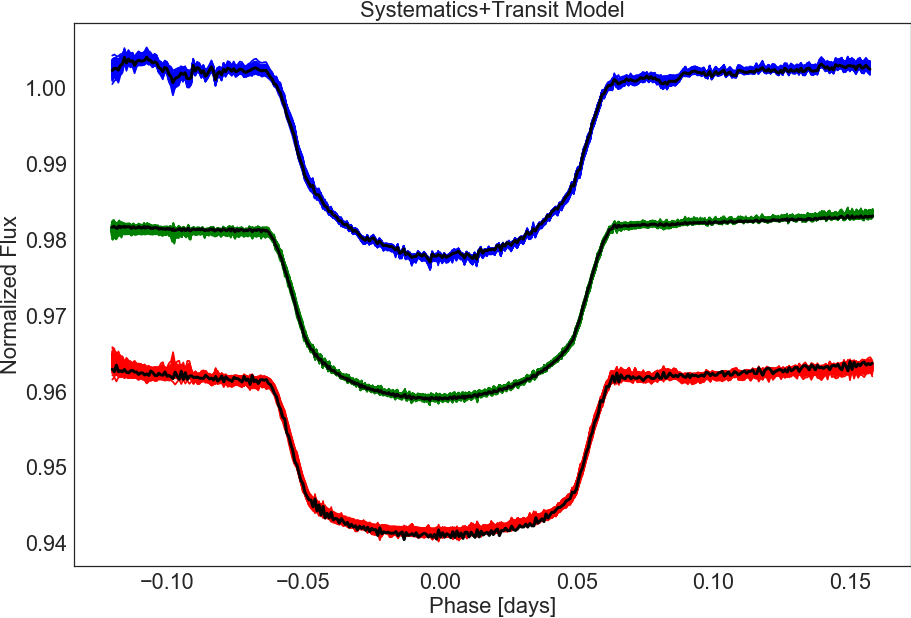
\includegraphics[width=7cm]{hatp44/transit_with_sys.png}
\caption{Full best-fit transit+systematics models.}
\end{subfigure}
\caption{(a) HAT-P-44b's best-fit transit models (black line) superposed with the systematics-corrected data (grey points). The colored lines are 1000 random samples that qualitatively show that the posterior distributions are sufficiently converged. The blue, green, and red correspond to g-,r-,and z-bands respectively. (b) Same as in (a) but with added systematics model.}
\label{fig:hatp44_samples}
\end{figure}

\begin{figure}
\centering
\begin{subfigure}{.5\textwidth}
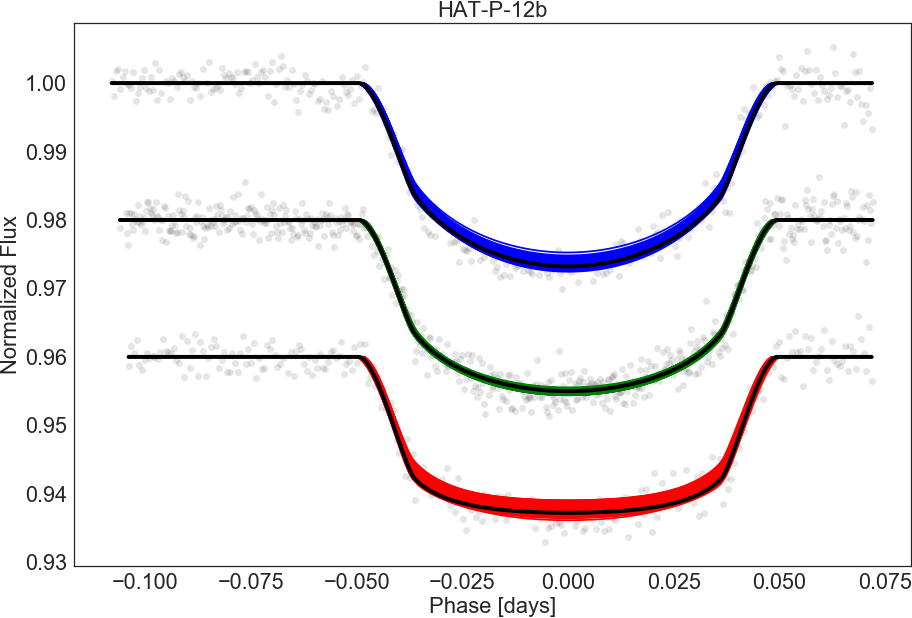
\includegraphics[width=7cm]{hatp12/1000_posterior_samples.png}
\caption{Full best-fit transit models.}
\end{subfigure}%
\begin{subfigure}{.5\textwidth}
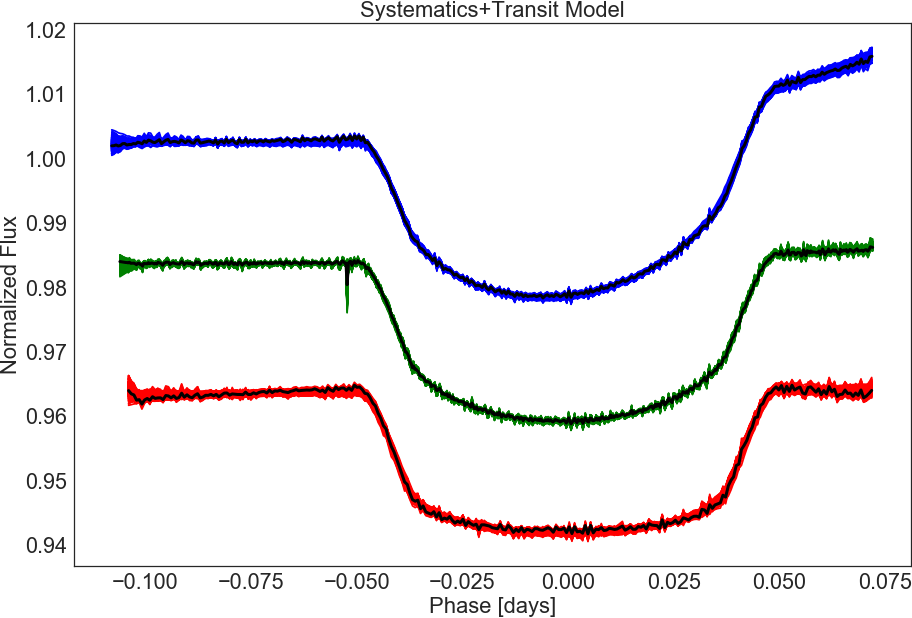
\includegraphics[width=7cm]{hatp12/transit_with_sys.png}
\caption{Full best-fit transit+systematics models.}
\end{subfigure}
\caption{Same as Fig.~\ref{fig:hatp44_samples} but for HAT-P-12b.}
\label{fig:hatp12_samples}
\end{figure}

\begin{figure}
\centering
\begin{subfigure}{.5\textwidth}
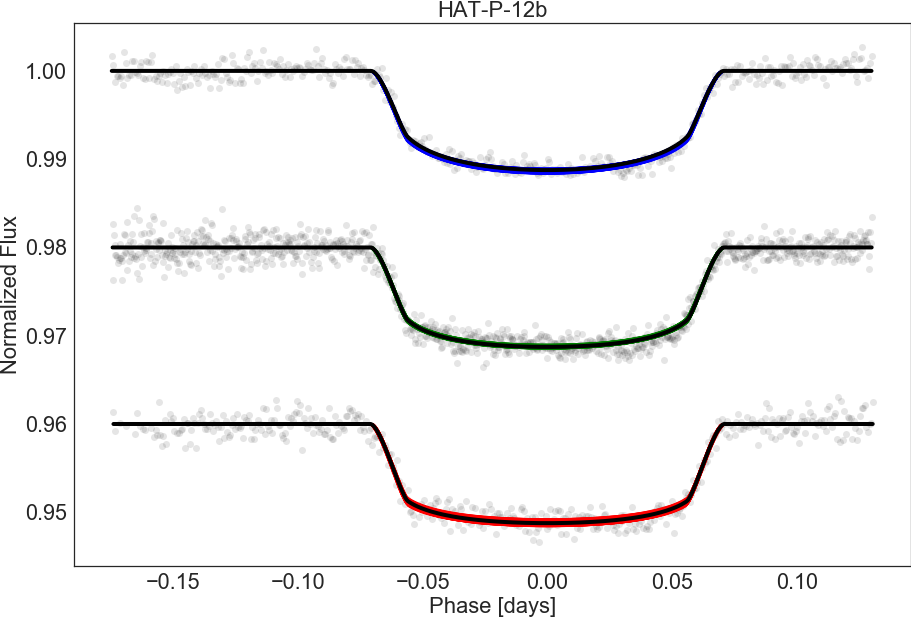
\includegraphics[width=7cm]{wasp21/1000_posterior_samples.png}
\caption{Full best-fit transit models.}
\end{subfigure}%
\begin{subfigure}{.5\textwidth}
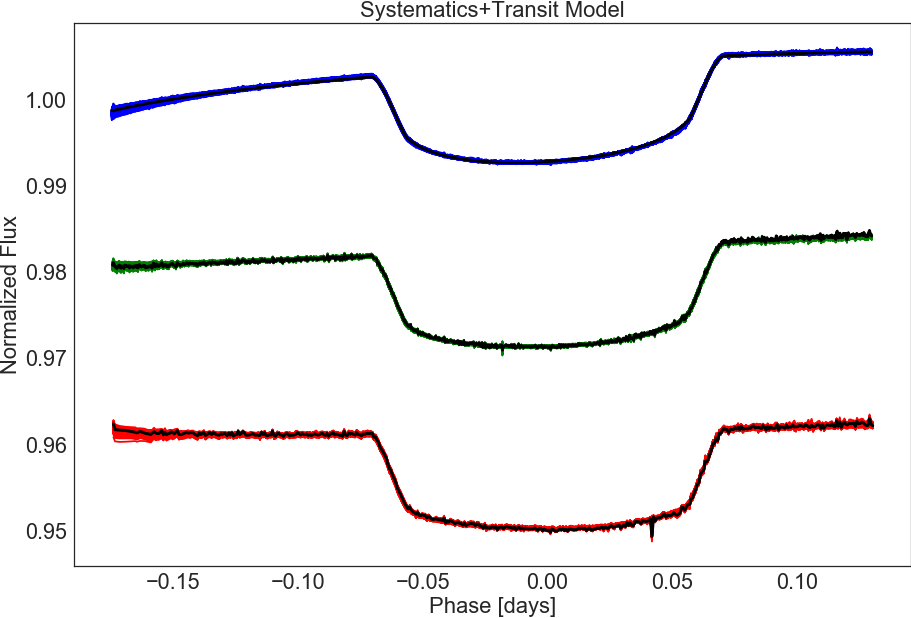
\includegraphics[width=7cm]{wasp21/transit_with_sys.png}
\caption{Full best-fit transit+systematics models.}
\end{subfigure}
\caption{Same as Fig.~\ref{fig:hatp44_samples} but for WASP-21b.}
\label{fig:wasp21_samples}
\end{figure}


%\paragraph{MuSCAT filter transmission curves}
\begin{figure}
\centering
	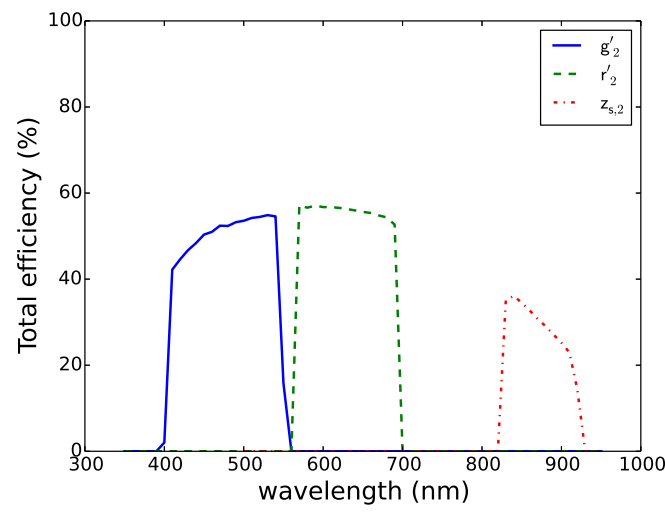
\includegraphics[width=10cm]{figures/MuSCAT_efficiency.png}
    \caption{Transmission curves of OAO/MuSCAT g', r', and z$_{s,2}$ filters. Each curves are integrated to determine the central wavelengths used in plotting the transmission spectrum and calculations.
    }\label{fig:filter_transmission}
\end{figure}

\begin{figure}
\centering
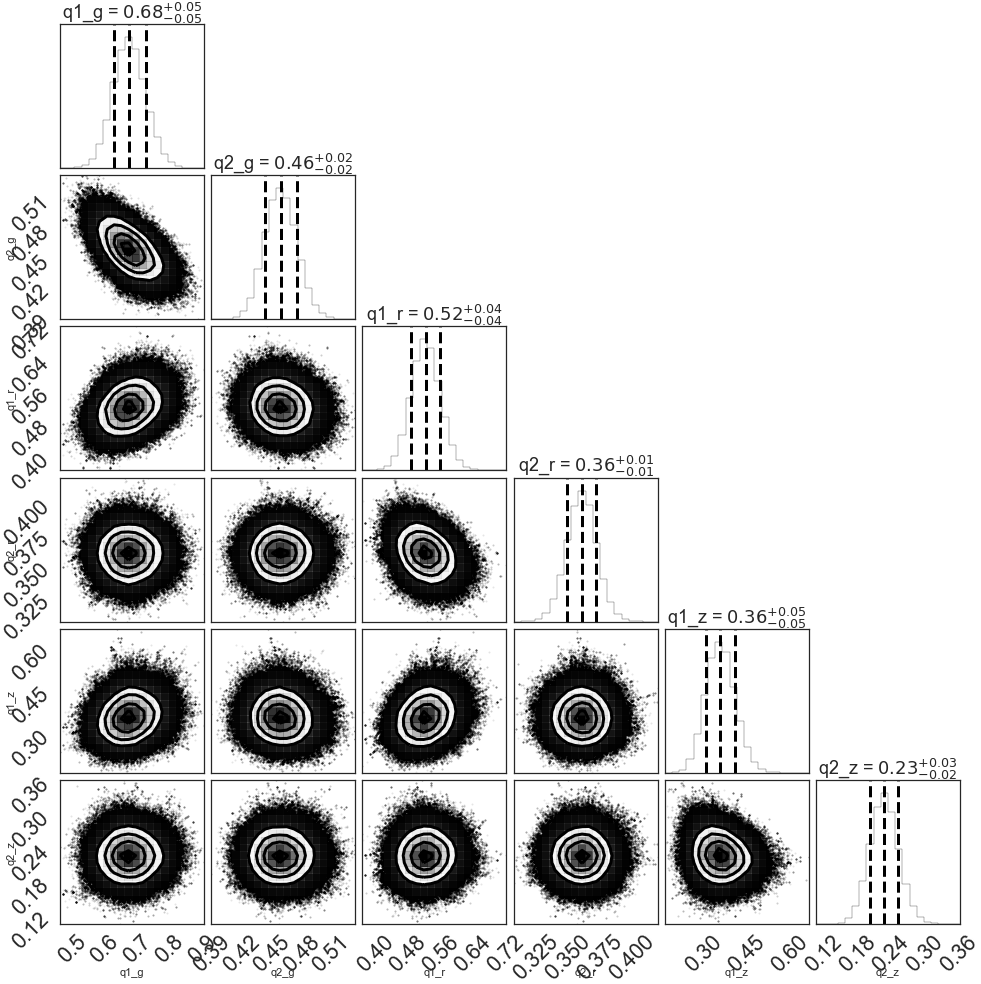
\includegraphics[width=7cm]{hatp44/limbdark_q1q2.png}
\caption{Corner plot of limb darkening coefficients showing joint posterior distributions along off-diagonal and marginalized distributions along the diagonal. As expected, there are no apparent correlations between limb darkening coefficients as shown by the joint plot.}
\label{fig:hatp44_q1q2}
\end{figure}

\begin{figure}
\centering
\includegraphics[width=7cm]{hatp12/limbdark_q1q2.png}
\caption{Same as Fig.~\ref{fig:hatp44_q1q2} but for HAT-P-12b.}
\label{fig:hatp12_q1q2}
\end{figure}


\begin{figure}
\centering
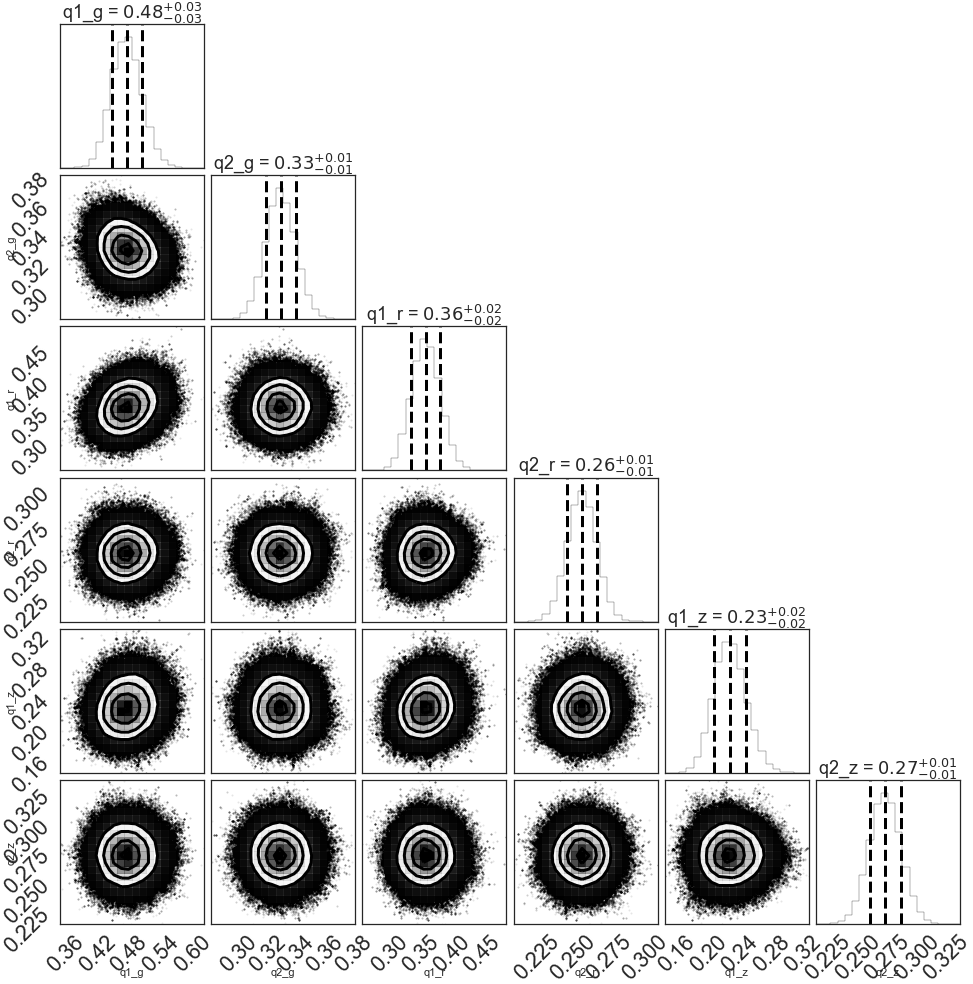
\includegraphics[width=7cm]{wasp21/limbdark_q1q2.png}
\caption{Same as Fig.~\ref{fig:hatp44_q1q2} but for WASP-21b.}
\label{fig:wasp21_q1q2}
\end{figure}

\begin{comment}
%\paragraph{Limb darkening}
%\setcounter{figure}{0}
\begin{figure}
\centering
\includegraphics[width=7cm]{figures/limbdark_blackbodies.png}
\caption{The upper black body corresponds to the solar disk (hotter) and the lower corresponds to the limb (cooler). As we go towards longer wavelengths (red), the ratio of the intensities (area bounded by each bandpasses) approaches 1, i.e. limb darkening effect is negligible in the infrared and more pronoounced in the optical. Thus, we expect to see the shape of z-band flatter than g-band.}
\label{fig:bb}
\end{figure}


\begin{figure}
\centering
\includegraphics[width=7cm]{figures/q_to_u.png}
\caption{Transformation of limb darkening coefficients between $q$- (blue) and $u$-space (red). This transformation constrains our sampling algorithm to explore only physically allowed limb-darkening coefficients, $u$, used to evaluate the Mandel-Agol model (See $\S$\ref{sec:transitmodel}).}
\label{fig:q_to_u}
\end{figure}
\end{comment}

\begin{comment}
\chapter{Model Selection}
We used the Bayes factor to select between competing models. The Bayesian evidence, $Z$, is defined by
\begin{equation}
Z=P(D|M)=\int d\theta P(\theta|M)P(D|\theta,M) 
\end{equation}
where $P(D|M)$ is the probability of observing the data $D$ given model $M$, marginalized over the model parameters $\theta$. The Bayes factor comparing the posterior probabilities for Models $M_1$ and $M_2$ given the data $D$ is defined by: 
\begin{equation}
 K_{1,2}=\frac{P(M_1|D)}{P(M_2|D}=\frac{P(M_1)P(D|M_1)}{P(M_2)P(D|M_2)}
\end{equation}
where P(M) is the prior probability for model $M$. Assuming equal priors for the different models tested, the Bayes factor is then equal to the evidence ratio:
\begin{equation}
 K_{1,2}=\frac{Z_1}{Z_2}
\end{equation}
If $ K_{1,2} > 1$, then $M_1$ is favored over model $M_2$.

In practice, $Z$ is difficult to determine as it requires integrating a complicated function over a high-dimensional space (e.g., Ferroz et al 2009). %https://arxiv.org/pdf/0809.3437.pdf
On the other hand, Weinberg et al. (2013) suggested a simple and relatively accurate method for estimating Z directly from the results of an MCMC simulation. 
\end{comment}

%---Other possible references
\bibliography{references}

%\end{CJK*}
\end{document}